\documentclass[twoside]{book}

% Packages required by doxygen
\usepackage{fixltx2e}
\usepackage{calc}
\usepackage{doxygen}
\usepackage[export]{adjustbox} % also loads graphicx
\usepackage{graphicx}
\usepackage[utf8]{inputenc}
\usepackage{makeidx}
\usepackage{multicol}
\usepackage{multirow}
\PassOptionsToPackage{warn}{textcomp}
\usepackage{textcomp}
\usepackage[nointegrals]{wasysym}
\usepackage[table]{xcolor}

% Font selection
\usepackage[T1]{fontenc}
\usepackage[scaled=.90]{helvet}
\usepackage{courier}
\usepackage{amssymb}
\usepackage{sectsty}
\renewcommand{\familydefault}{\sfdefault}
\allsectionsfont{%
  \fontseries{bc}\selectfont%
  \color{darkgray}%
}
\renewcommand{\DoxyLabelFont}{%
  \fontseries{bc}\selectfont%
  \color{darkgray}%
}
\newcommand{\+}{\discretionary{\mbox{\scriptsize$\hookleftarrow$}}{}{}}

% Page & text layout
\usepackage{geometry}
\geometry{%
  a4paper,%
  top=2.5cm,%
  bottom=2.5cm,%
  left=2.5cm,%
  right=2.5cm%
}
\tolerance=750
\hfuzz=15pt
\hbadness=750
\setlength{\emergencystretch}{15pt}
\setlength{\parindent}{0cm}
\setlength{\parskip}{3ex plus 2ex minus 2ex}
\makeatletter
\renewcommand{\paragraph}{%
  \@startsection{paragraph}{4}{0ex}{-1.0ex}{1.0ex}{%
    \normalfont\normalsize\bfseries\SS@parafont%
  }%
}
\renewcommand{\subparagraph}{%
  \@startsection{subparagraph}{5}{0ex}{-1.0ex}{1.0ex}{%
    \normalfont\normalsize\bfseries\SS@subparafont%
  }%
}
\makeatother

% Headers & footers
\usepackage{fancyhdr}
\pagestyle{fancyplain}
\fancyhead[LE]{\fancyplain{}{\bfseries\thepage}}
\fancyhead[CE]{\fancyplain{}{}}
\fancyhead[RE]{\fancyplain{}{\bfseries\leftmark}}
\fancyhead[LO]{\fancyplain{}{\bfseries\rightmark}}
\fancyhead[CO]{\fancyplain{}{}}
\fancyhead[RO]{\fancyplain{}{\bfseries\thepage}}
\fancyfoot[LE]{\fancyplain{}{}}
\fancyfoot[CE]{\fancyplain{}{}}
\fancyfoot[RE]{\fancyplain{}{\bfseries\scriptsize Generated by Doxygen }}
\fancyfoot[LO]{\fancyplain{}{\bfseries\scriptsize Generated by Doxygen }}
\fancyfoot[CO]{\fancyplain{}{}}
\fancyfoot[RO]{\fancyplain{}{}}
\renewcommand{\footrulewidth}{0.4pt}
\renewcommand{\chaptermark}[1]{%
  \markboth{#1}{}%
}
\renewcommand{\sectionmark}[1]{%
  \markright{\thesection\ #1}%
}

% Indices & bibliography
\usepackage{natbib}
\usepackage[titles]{tocloft}
\setcounter{tocdepth}{3}
\setcounter{secnumdepth}{5}
\makeindex

% Hyperlinks (required, but should be loaded last)
\usepackage{ifpdf}
\ifpdf
  \usepackage[pdftex,pagebackref=true]{hyperref}
\else
  \usepackage[ps2pdf,pagebackref=true]{hyperref}
\fi
\hypersetup{%
  colorlinks=true,%
  linkcolor=blue,%
  citecolor=blue,%
  unicode%
}

% Custom commands
\newcommand{\clearemptydoublepage}{%
  \newpage{\pagestyle{empty}\cleardoublepage}%
}

\usepackage{caption}
\captionsetup{labelsep=space,justification=centering,font={bf},singlelinecheck=off,skip=4pt,position=top}

%===== C O N T E N T S =====

\begin{document}

% Titlepage & ToC
\hypersetup{pageanchor=false,
             bookmarksnumbered=true,
             pdfencoding=unicode
            }
\pagenumbering{alph}
\begin{titlepage}
\vspace*{7cm}
\begin{center}%
{\Large Aircraft\+\_\+carrier\+\_\+group }\\
\vspace*{1cm}
{\large Generated by Doxygen 1.8.14}\\
\end{center}
\end{titlepage}
\clearemptydoublepage
\pagenumbering{roman}
\tableofcontents
\clearemptydoublepage
\pagenumbering{arabic}
\hypersetup{pageanchor=true}

%--- Begin generated contents ---
\chapter{Namespace Index}
\section{Namespace List}
Here is a list of all documented namespaces with brief descriptions\+:\begin{DoxyCompactList}
\item\contentsline{section}{\mbox{\hyperlink{namespace_aircraft_carrier_group}{Aircraft\+Carrier\+Group}} \\*Пространство имен \mbox{\hyperlink{namespace_aircraft_carrier_group}{Aircraft\+Carrier\+Group}} }{\pageref{namespace_aircraft_carrier_group}}{}
\end{DoxyCompactList}

\chapter{Hierarchical Index}
\section{Class Hierarchy}
This inheritance list is sorted roughly, but not completely, alphabetically\+:\begin{DoxyCompactList}
\item \contentsline{section}{\+\_\+map$<$ key, info $>$}{\pageref{class__map}}{}
\item \contentsline{section}{\+\_\+map$<$ std\+:\+:string, Aircraft\+Carrier\+Group\+:\+:Ship $\ast$$>$}{\pageref{class__map}}{}
\item \contentsline{section}{\+\_\+map\+\_\+iterator$<$ key, info $>$}{\pageref{class__map__iterator}}{}
\item \contentsline{section}{\+\_\+pair$<$ key, info $>$}{\pageref{struct__pair}}{}
\item \contentsline{section}{\+\_\+pair$<$ std\+:\+:string, Aircraft\+Carrier\+Group\+:\+:Ship $\ast$$>$}{\pageref{struct__pair}}{}
\item \contentsline{section}{Aircraft\+Carrier\+Group\+:\+:Captain}{\pageref{struct_aircraft_carrier_group_1_1_captain}}{}
\item \contentsline{section}{Aircraft\+Carrier\+Group\+:\+:Const\+Fleet\+It}{\pageref{class_aircraft_carrier_group_1_1_const_fleet_it}}{}
\item \contentsline{section}{Aircraft\+Carrier\+Group\+:\+:Fleet}{\pageref{class_aircraft_carrier_group_1_1_fleet}}{}
\item \contentsline{section}{Aircraft\+Carrier\+Group\+:\+:Military\+Characteristics}{\pageref{class_aircraft_carrier_group_1_1_military_characteristics}}{}
\begin{DoxyCompactList}
\item \contentsline{section}{Aircraft\+Carrier\+Group\+:\+:Aircraft}{\pageref{class_aircraft_carrier_group_1_1_aircraft}}{}
\item \contentsline{section}{Aircraft\+Carrier\+Group\+:\+:Ship}{\pageref{class_aircraft_carrier_group_1_1_ship}}{}
\begin{DoxyCompactList}
\item \contentsline{section}{Aircraft\+Carrier\+Group\+:\+:Carrier}{\pageref{class_aircraft_carrier_group_1_1_carrier}}{}
\begin{DoxyCompactList}
\item \contentsline{section}{Aircraft\+Carrier\+Group\+:\+:Aircraft\+Carrier}{\pageref{class_aircraft_carrier_group_1_1_aircraft_carrier}}{}
\end{DoxyCompactList}
\item \contentsline{section}{Aircraft\+Carrier\+Group\+:\+:Cover\+Ship}{\pageref{class_aircraft_carrier_group_1_1_cover_ship}}{}
\end{DoxyCompactList}
\end{DoxyCompactList}
\item \contentsline{section}{Aircraft\+Carrier\+Group\+:\+:Weapon}{\pageref{class_aircraft_carrier_group_1_1_weapon}}{}
\end{DoxyCompactList}

\chapter{Class Index}
\section{Class List}
Here are the classes, structs, unions and interfaces with brief descriptions\+:\begin{DoxyCompactList}
\item\contentsline{section}{\mbox{\hyperlink{class__map}{\+\_\+map$<$ key, info $>$}} }{\pageref{class__map}}{}
\item\contentsline{section}{\mbox{\hyperlink{class__map__iterator}{\+\_\+map\+\_\+iterator$<$ key, info $>$}} }{\pageref{class__map__iterator}}{}
\item\contentsline{section}{\mbox{\hyperlink{struct__pair}{\+\_\+pair$<$ key, info $>$}} }{\pageref{struct__pair}}{}
\item\contentsline{section}{\mbox{\hyperlink{class_aircraft_carrier_group_1_1_aircraft}{Aircraft\+Carrier\+Group\+::\+Aircraft}} \\*Класс для описания самолета  Осуществляет хранение всех параметров самолета и содержит функции, обрабатывающие эти параметры }{\pageref{class_aircraft_carrier_group_1_1_aircraft}}{}
\item\contentsline{section}{\mbox{\hyperlink{class_aircraft_carrier_group_1_1_aircraft_carrier}{Aircraft\+Carrier\+Group\+::\+Aircraft\+Carrier}} \\*Класс для описания авианесущего крейсера  Осуществляет хранение всех параметров авианесущего крейсера и содержит функции, обрабатывающие эти параметры }{\pageref{class_aircraft_carrier_group_1_1_aircraft_carrier}}{}
\item\contentsline{section}{\mbox{\hyperlink{struct_aircraft_carrier_group_1_1_captain}{Aircraft\+Carrier\+Group\+::\+Captain}} \\*Структура для описания капитана  Осуществляет хранение всех параметров командира судна или флота }{\pageref{struct_aircraft_carrier_group_1_1_captain}}{}
\item\contentsline{section}{\mbox{\hyperlink{class_aircraft_carrier_group_1_1_carrier}{Aircraft\+Carrier\+Group\+::\+Carrier}} \\*Класс для описания авианосца  Осуществляет хранение всех параметров авиносца и содержит функции, обрабатывающие эти параметры }{\pageref{class_aircraft_carrier_group_1_1_carrier}}{}
\item\contentsline{section}{\mbox{\hyperlink{class_aircraft_carrier_group_1_1_const_fleet_it}{Aircraft\+Carrier\+Group\+::\+Const\+Fleet\+It}} \\*Класс-\/итератор для класса \mbox{\hyperlink{class_aircraft_carrier_group_1_1_fleet}{Fleet}}  При его помощи осуществляется доступ к элементам контейнера класса \mbox{\hyperlink{class_aircraft_carrier_group_1_1_fleet}{Fleet}} }{\pageref{class_aircraft_carrier_group_1_1_const_fleet_it}}{}
\item\contentsline{section}{\mbox{\hyperlink{class_aircraft_carrier_group_1_1_cover_ship}{Aircraft\+Carrier\+Group\+::\+Cover\+Ship}} \\*Класс для описания судна прикрытия  Осуществляет хранение всех параметров судна прикрытия и содержит функции, обрабатывающие эти параметры }{\pageref{class_aircraft_carrier_group_1_1_cover_ship}}{}
\item\contentsline{section}{\mbox{\hyperlink{class_aircraft_carrier_group_1_1_fleet}{Aircraft\+Carrier\+Group\+::\+Fleet}} \\*Класс для описания флота  Осуществляет хранение описателей всех кораблей флота и содержит функции, позволяющие взаимодействовать с кораблями флота }{\pageref{class_aircraft_carrier_group_1_1_fleet}}{}
\item\contentsline{section}{\mbox{\hyperlink{class_aircraft_carrier_group_1_1_military_characteristics}{Aircraft\+Carrier\+Group\+::\+Military\+Characteristics}} \\*Класс для описания некоторых парметров техники  Осуществляет хранение и обработку некоторых характеристик техники }{\pageref{class_aircraft_carrier_group_1_1_military_characteristics}}{}
\item\contentsline{section}{\mbox{\hyperlink{class_aircraft_carrier_group_1_1_ship}{Aircraft\+Carrier\+Group\+::\+Ship}} \\*Абстрактный класс для описания кораблей  Осуществляет хранение общих параметров кораблей и содержит функции, обрабатывающие эти параметры }{\pageref{class_aircraft_carrier_group_1_1_ship}}{}
\item\contentsline{section}{\mbox{\hyperlink{class_aircraft_carrier_group_1_1_weapon}{Aircraft\+Carrier\+Group\+::\+Weapon}} \\*Класс для описания вооружения  Осуществляет хранение всех параметров авианесущего крейсера и содержит функции, обрабатывающие эти параметры }{\pageref{class_aircraft_carrier_group_1_1_weapon}}{}
\end{DoxyCompactList}

\chapter{File Index}
\section{File List}
Here is a list of all documented files with brief descriptions\+:\begin{DoxyCompactList}
\item\contentsline{section}{C\+:/\+Users/\+Sema/\+Desktop/\+Code\+Forces/\+Labs/4th\+\_\+\+Lab + library connection/\+Library/{\bfseries \+\_\+map.\+h} }{\pageref{__map_8h}}{}
\item\contentsline{section}{C\+:/\+Users/\+Sema/\+Desktop/\+Code\+Forces/\+Labs/4th\+\_\+\+Lab + library connection/\+Library/\mbox{\hyperlink{_aircraft_8h}{Aircraft.\+h}} \\*Заголовочный файл с описанием класса  Данный файл содержит в себе определение класса Aircraft }{\pageref{_aircraft_8h}}{}
\item\contentsline{section}{C\+:/\+Users/\+Sema/\+Desktop/\+Code\+Forces/\+Labs/4th\+\_\+\+Lab + library connection/\+Library/\mbox{\hyperlink{_aircraft_carrier_8h}{Aircraft\+Carrier.\+h}} \\*Заголовочный файл с описанием класса  Данный файл содержит в себе определение класса Aircraft\+Carrier }{\pageref{_aircraft_carrier_8h}}{}
\item\contentsline{section}{C\+:/\+Users/\+Sema/\+Desktop/\+Code\+Forces/\+Labs/4th\+\_\+\+Lab + library connection/\+Library/\mbox{\hyperlink{_carrier_8h}{Carrier.\+h}} \\*Заголовочный файл с описанием класса  Данный файл содержит в себе определение класса Carrier }{\pageref{_carrier_8h}}{}
\item\contentsline{section}{C\+:/\+Users/\+Sema/\+Desktop/\+Code\+Forces/\+Labs/4th\+\_\+\+Lab + library connection/\+Library/\mbox{\hyperlink{_cover_ship_8h}{Cover\+Ship.\+h}} \\*Заголовочный файл с описанием класса  Данный файл содержит в себе определение класса Cover\+Ship }{\pageref{_cover_ship_8h}}{}
\item\contentsline{section}{C\+:/\+Users/\+Sema/\+Desktop/\+Code\+Forces/\+Labs/4th\+\_\+\+Lab + library connection/\+Library/\mbox{\hyperlink{_fleet_8h}{Fleet.\+h}} \\*Заголовочный файл с описанием класса и его итератора  Данный файл содержит в себе определение класса Fleet }{\pageref{_fleet_8h}}{}
\item\contentsline{section}{C\+:/\+Users/\+Sema/\+Desktop/\+Code\+Forces/\+Labs/4th\+\_\+\+Lab + library connection/\+Library/\mbox{\hyperlink{_military_characteristics_8h}{Military\+Characteristics.\+h}} \\*Заголовочный файл с описанием класса  Данный файл содержит в себе определение класса Military\+Characteristics }{\pageref{_military_characteristics_8h}}{}
\item\contentsline{section}{C\+:/\+Users/\+Sema/\+Desktop/\+Code\+Forces/\+Labs/4th\+\_\+\+Lab + library connection/\+Library/\mbox{\hyperlink{_ship_8h}{Ship.\+h}} \\*Заголовочный файл с описанием класса  Данный файл содержит в себе определение класса Cover\+Ship }{\pageref{_ship_8h}}{}
\item\contentsline{section}{C\+:/\+Users/\+Sema/\+Desktop/\+Code\+Forces/\+Labs/4th\+\_\+\+Lab + library connection/\+Library/{\bfseries stdafx.\+h} }{\pageref{stdafx_8h}}{}
\item\contentsline{section}{C\+:/\+Users/\+Sema/\+Desktop/\+Code\+Forces/\+Labs/4th\+\_\+\+Lab + library connection/\+Library/{\bfseries targetver.\+h} }{\pageref{targetver_8h}}{}
\item\contentsline{section}{C\+:/\+Users/\+Sema/\+Desktop/\+Code\+Forces/\+Labs/4th\+\_\+\+Lab + library connection/\+Library/\mbox{\hyperlink{_weapon_8h}{Weapon.\+h}} \\*Заголовочный файл с описанием класса  Данный файл содержит в себе определение класса Weapon }{\pageref{_weapon_8h}}{}
\end{DoxyCompactList}

\chapter{Namespace Documentation}
\hypertarget{namespace_aircraft_carrier_group}{}\section{Aircraft\+Carrier\+Group Namespace Reference}
\label{namespace_aircraft_carrier_group}\index{Aircraft\+Carrier\+Group@{Aircraft\+Carrier\+Group}}


Пространство имен \mbox{\hyperlink{namespace_aircraft_carrier_group}{Aircraft\+Carrier\+Group}}.  


\subsection*{Classes}
\begin{DoxyCompactItemize}
\item 
class \mbox{\hyperlink{class_aircraft_carrier_group_1_1_aircraft}{Aircraft}}
\begin{DoxyCompactList}\small\item\em Класс для описания самолета  Осуществляет хранение всех параметров самолета и содержит функции, обрабатывающие эти параметры \end{DoxyCompactList}\item 
class \mbox{\hyperlink{class_aircraft_carrier_group_1_1_aircraft_carrier}{Aircraft\+Carrier}}
\begin{DoxyCompactList}\small\item\em Класс для описания авианесущего крейсера  Осуществляет хранение всех параметров авианесущего крейсера и содержит функции, обрабатывающие эти параметры \end{DoxyCompactList}\item 
struct \mbox{\hyperlink{struct_aircraft_carrier_group_1_1_captain}{Captain}}
\begin{DoxyCompactList}\small\item\em Структура для описания капитана  Осуществляет хранение всех параметров командира судна или флота \end{DoxyCompactList}\item 
class \mbox{\hyperlink{class_aircraft_carrier_group_1_1_carrier}{Carrier}}
\begin{DoxyCompactList}\small\item\em Класс для описания авианосца  Осуществляет хранение всех параметров авиносца и содержит функции, обрабатывающие эти параметры \end{DoxyCompactList}\item 
class \mbox{\hyperlink{class_aircraft_carrier_group_1_1_const_fleet_it}{Const\+Fleet\+It}}
\begin{DoxyCompactList}\small\item\em Класс-\/итератор для класса \mbox{\hyperlink{class_aircraft_carrier_group_1_1_fleet}{Fleet}}  При его помощи осуществляется доступ к элементам контейнера класса \mbox{\hyperlink{class_aircraft_carrier_group_1_1_fleet}{Fleet}}. \end{DoxyCompactList}\item 
class \mbox{\hyperlink{class_aircraft_carrier_group_1_1_cover_ship}{Cover\+Ship}}
\begin{DoxyCompactList}\small\item\em Класс для описания судна прикрытия  Осуществляет хранение всех параметров судна прикрытия и содержит функции, обрабатывающие эти параметры \end{DoxyCompactList}\item 
class \mbox{\hyperlink{class_aircraft_carrier_group_1_1_fleet}{Fleet}}
\begin{DoxyCompactList}\small\item\em Класс для описания флота  Осуществляет хранение описателей всех кораблей флота и содержит функции, позволяющие взаимодействовать с кораблями флота \end{DoxyCompactList}\item 
class \mbox{\hyperlink{class_aircraft_carrier_group_1_1_military_characteristics}{Military\+Characteristics}}
\begin{DoxyCompactList}\small\item\em Класс для описания некоторых парметров техники  Осуществляет хранение и обработку некоторых характеристик техники \end{DoxyCompactList}\item 
class \mbox{\hyperlink{class_aircraft_carrier_group_1_1_ship}{Ship}}
\begin{DoxyCompactList}\small\item\em Абстрактный класс для описания кораблей  Осуществляет хранение общих параметров кораблей и содержит функции, обрабатывающие эти параметры \end{DoxyCompactList}\item 
class \mbox{\hyperlink{class_aircraft_carrier_group_1_1_weapon}{Weapon}}
\begin{DoxyCompactList}\small\item\em Класс для описания вооружения  Осуществляет хранение всех параметров авианесущего крейсера и содержит функции, обрабатывающие эти параметры \end{DoxyCompactList}\end{DoxyCompactItemize}
\subsection*{Functions}
\begin{DoxyCompactItemize}
\item 
\mbox{\Hypertarget{namespace_aircraft_carrier_group_a7086b798964cb013d658074468fbf7b9}\label{namespace_aircraft_carrier_group_a7086b798964cb013d658074468fbf7b9}} 
std\+::ostream \& {\bfseries operator$<$$<$} (std\+::ostream \&os, const \mbox{\hyperlink{class_aircraft_carrier_group_1_1_aircraft}{Aircraft}} \&Plane)
\item 
\mbox{\Hypertarget{namespace_aircraft_carrier_group_acb10365ad0985a5893d722e262903059}\label{namespace_aircraft_carrier_group_acb10365ad0985a5893d722e262903059}} 
std\+::istream \& {\bfseries operator$>$$>$} (std\+::istream \&is, \mbox{\hyperlink{class_aircraft_carrier_group_1_1_aircraft}{Aircraft}} \&Plane)
\item 
\mbox{\Hypertarget{namespace_aircraft_carrier_group_a22ed3a3a46c0fd896e01fd071ad3b9e9}\label{namespace_aircraft_carrier_group_a22ed3a3a46c0fd896e01fd071ad3b9e9}} 
std\+::ifstream \& {\bfseries operator$>$$>$} (std\+::ifstream \&is, \mbox{\hyperlink{class_aircraft_carrier_group_1_1_aircraft}{Aircraft}} \&Plane)
\item 
\mbox{\Hypertarget{namespace_aircraft_carrier_group_a69e1ec2fd6a45ba545ec6ff0f3e0b286}\label{namespace_aircraft_carrier_group_a69e1ec2fd6a45ba545ec6ff0f3e0b286}} 
std\+::ofstream \& {\bfseries operator$<$$<$} (std\+::ofstream \&os, const \mbox{\hyperlink{class_aircraft_carrier_group_1_1_aircraft}{Aircraft}} \&Plane)
\item 
\mbox{\Hypertarget{namespace_aircraft_carrier_group_aed5832cc1645fd6462a85d7a822a9b4e}\label{namespace_aircraft_carrier_group_aed5832cc1645fd6462a85d7a822a9b4e}} 
std\+::istream \& {\bfseries operator$>$$>$} (std\+::istream \&is, \mbox{\hyperlink{class_aircraft_carrier_group_1_1_aircraft_carrier}{Aircraft\+Carrier}} \&Aerocarrier\+Tmp)
\item 
\mbox{\Hypertarget{namespace_aircraft_carrier_group_af4d1dd1af14f671fd8fa30824a279938}\label{namespace_aircraft_carrier_group_af4d1dd1af14f671fd8fa30824a279938}} 
std\+::ostream \& {\bfseries operator$<$$<$} (std\+::ostream \&os, const \mbox{\hyperlink{class_aircraft_carrier_group_1_1_aircraft_carrier}{Aircraft\+Carrier}} \&Aerocarrier\+Tmp)
\item 
\mbox{\Hypertarget{namespace_aircraft_carrier_group_a2978940c703df25a3a5a452389495b16}\label{namespace_aircraft_carrier_group_a2978940c703df25a3a5a452389495b16}} 
std\+::istream \& {\bfseries operator$>$$>$} (std\+::istream \&is, \mbox{\hyperlink{class_aircraft_carrier_group_1_1_carrier}{Carrier}} \&Carrier\+Tmp)
\item 
\mbox{\Hypertarget{namespace_aircraft_carrier_group_ab8fbe9afd8dfc9641502d161226cc2e8}\label{namespace_aircraft_carrier_group_ab8fbe9afd8dfc9641502d161226cc2e8}} 
std\+::ostream \& {\bfseries operator$<$$<$} (std\+::ostream \&os, const \mbox{\hyperlink{class_aircraft_carrier_group_1_1_carrier}{Carrier}} \&Carrier\+Tmp)
\item 
\mbox{\Hypertarget{namespace_aircraft_carrier_group_abb71ecf9d793b33322cb112051a66232}\label{namespace_aircraft_carrier_group_abb71ecf9d793b33322cb112051a66232}} 
std\+::istream \& {\bfseries operator$>$$>$} (std\+::istream \&is, \mbox{\hyperlink{class_aircraft_carrier_group_1_1_cover_ship}{Cover\+Ship}} \&Cover\+Ship\+Tmp)
\item 
\mbox{\Hypertarget{namespace_aircraft_carrier_group_a8fee94b9f1245a2f7ba4ad8dcc61cd72}\label{namespace_aircraft_carrier_group_a8fee94b9f1245a2f7ba4ad8dcc61cd72}} 
std\+::ostream \& {\bfseries operator$<$$<$} (std\+::ostream \&os, const \mbox{\hyperlink{class_aircraft_carrier_group_1_1_cover_ship}{Cover\+Ship}} \&Cover\+Ship\+Tmp)
\item 
\mbox{\Hypertarget{namespace_aircraft_carrier_group_a9f43a9994a583702541778ae23677677}\label{namespace_aircraft_carrier_group_a9f43a9994a583702541778ae23677677}} 
std\+::ostream \& {\bfseries operator$<$$<$} (std\+::ostream \&os, const std\+::pair$<$ const std\+::string, \mbox{\hyperlink{class_aircraft_carrier_group_1_1_ship}{Ship}} $\ast$$>$ \&ptr)
\item 
\mbox{\Hypertarget{namespace_aircraft_carrier_group_a6e801e9f18142a151bbd3740162b3b0a}\label{namespace_aircraft_carrier_group_a6e801e9f18142a151bbd3740162b3b0a}} 
std\+::ifstream \& {\bfseries operator$>$$>$} (std\+::ifstream \&is, \mbox{\hyperlink{class_aircraft_carrier_group_1_1_fleet}{Fleet}} \&Fleet\+Tmp)
\item 
\mbox{\Hypertarget{namespace_aircraft_carrier_group_a1d4a32e23093ecd31e69d403e87a8cad}\label{namespace_aircraft_carrier_group_a1d4a32e23093ecd31e69d403e87a8cad}} 
std\+::ofstream \& {\bfseries operator$<$$<$} (std\+::ofstream \&os, const \mbox{\hyperlink{class_aircraft_carrier_group_1_1_fleet}{Fleet}} \&Fleet\+Tmp)
\item 
\mbox{\Hypertarget{namespace_aircraft_carrier_group_a041b295ea5def9c25a529ac316c266ef}\label{namespace_aircraft_carrier_group_a041b295ea5def9c25a529ac316c266ef}} 
std\+::ostream \& {\bfseries operator$<$$<$} (std\+::ostream \&os, const \mbox{\hyperlink{class_aircraft_carrier_group_1_1_fleet}{Fleet}} \&Fleet\+Tmp)
\item 
\mbox{\Hypertarget{namespace_aircraft_carrier_group_a0a3f6c21388e2340bdc42cde5a8dd46f}\label{namespace_aircraft_carrier_group_a0a3f6c21388e2340bdc42cde5a8dd46f}} 
std\+::ostream \& {\bfseries operator$<$$<$} (std\+::ostream \&os, const \mbox{\hyperlink{class_aircraft_carrier_group_1_1_military_characteristics}{Military\+Characteristics}} \&Military)
\item 
\mbox{\Hypertarget{namespace_aircraft_carrier_group_a20d275ddadea86402ea52f13f31032d5}\label{namespace_aircraft_carrier_group_a20d275ddadea86402ea52f13f31032d5}} 
std\+::istream \& {\bfseries operator$>$$>$} (std\+::istream \&is, \mbox{\hyperlink{class_aircraft_carrier_group_1_1_military_characteristics}{Military\+Characteristics}} \&Military)
\item 
\mbox{\Hypertarget{namespace_aircraft_carrier_group_acf1703e4cf597fc4befb12f0771b41a1}\label{namespace_aircraft_carrier_group_acf1703e4cf597fc4befb12f0771b41a1}} 
std\+::ifstream \& {\bfseries operator$>$$>$} (std\+::ifstream \&is, \mbox{\hyperlink{class_aircraft_carrier_group_1_1_military_characteristics}{Military\+Characteristics}} \&Military)
\item 
\mbox{\Hypertarget{namespace_aircraft_carrier_group_aa2cdde6ecea4f7c9c76f90548a95fbda}\label{namespace_aircraft_carrier_group_aa2cdde6ecea4f7c9c76f90548a95fbda}} 
std\+::ofstream \& {\bfseries operator$<$$<$} (std\+::ofstream \&os, const \mbox{\hyperlink{class_aircraft_carrier_group_1_1_military_characteristics}{Military\+Characteristics}} \&Military)
\item 
\mbox{\Hypertarget{namespace_aircraft_carrier_group_a513daf0489f219fe029fa20094d394da}\label{namespace_aircraft_carrier_group_a513daf0489f219fe029fa20094d394da}} 
std\+::istream \& {\bfseries operator$>$$>$} (std\+::istream \&is, \mbox{\hyperlink{struct_aircraft_carrier_group_1_1_captain}{Captain}} \&Commander)
\item 
\mbox{\Hypertarget{namespace_aircraft_carrier_group_a5056a8d42f6683e8ac1f004b1a024f2b}\label{namespace_aircraft_carrier_group_a5056a8d42f6683e8ac1f004b1a024f2b}} 
std\+::ostream \& {\bfseries operator$<$$<$} (std\+::ostream \&os, const \mbox{\hyperlink{struct_aircraft_carrier_group_1_1_captain}{Captain}} \&Commander)
\item 
\mbox{\Hypertarget{namespace_aircraft_carrier_group_ae3b1717032e40b76a5cfe0d15f241cf9}\label{namespace_aircraft_carrier_group_ae3b1717032e40b76a5cfe0d15f241cf9}} 
std\+::ifstream \& {\bfseries operator$>$$>$} (std\+::ifstream \&is, \mbox{\hyperlink{struct_aircraft_carrier_group_1_1_captain}{Captain}} \&Commander)
\item 
\mbox{\Hypertarget{namespace_aircraft_carrier_group_abe06f32467ae0067f2c206f5033492c9}\label{namespace_aircraft_carrier_group_abe06f32467ae0067f2c206f5033492c9}} 
std\+::ofstream \& {\bfseries operator$<$$<$} (std\+::ofstream \&os, const \mbox{\hyperlink{struct_aircraft_carrier_group_1_1_captain}{Captain}} \&Commander)
\item 
\mbox{\Hypertarget{namespace_aircraft_carrier_group_a95ec58ec6070dd4cec3008ef366f0573}\label{namespace_aircraft_carrier_group_a95ec58ec6070dd4cec3008ef366f0573}} 
std\+::ostream \& {\bfseries operator$<$$<$} (std\+::ostream \&os, const \mbox{\hyperlink{class_aircraft_carrier_group_1_1_weapon}{Weapon}} \&Arsenal)
\item 
\mbox{\Hypertarget{namespace_aircraft_carrier_group_a22724b26d62acbbb6a2e11e25396f182}\label{namespace_aircraft_carrier_group_a22724b26d62acbbb6a2e11e25396f182}} 
std\+::istream \& {\bfseries operator$>$$>$} (std\+::istream \&is, \mbox{\hyperlink{class_aircraft_carrier_group_1_1_weapon}{Weapon}} \&Arsenal)
\item 
\mbox{\Hypertarget{namespace_aircraft_carrier_group_afbb32142a113b66b4ca1e1b349a34cee}\label{namespace_aircraft_carrier_group_afbb32142a113b66b4ca1e1b349a34cee}} 
std\+::ifstream \& {\bfseries operator$>$$>$} (std\+::ifstream \&is, \mbox{\hyperlink{class_aircraft_carrier_group_1_1_weapon}{Weapon}} \&Arsenal)
\item 
\mbox{\Hypertarget{namespace_aircraft_carrier_group_a43a8c4b863d42762174e25ec9469121f}\label{namespace_aircraft_carrier_group_a43a8c4b863d42762174e25ec9469121f}} 
std\+::ofstream \& {\bfseries operator$<$$<$} (std\+::ofstream \&os, const \mbox{\hyperlink{class_aircraft_carrier_group_1_1_weapon}{Weapon}} \&Arsenal)
\end{DoxyCompactItemize}
\subsection*{Variables}
\begin{DoxyCompactItemize}
\item 
\mbox{\Hypertarget{namespace_aircraft_carrier_group_a450635cd66c0fbcc37535160a56142b8}\label{namespace_aircraft_carrier_group_a450635cd66c0fbcc37535160a56142b8}} 
const double {\bfseries eps} = 1e-\/9
\end{DoxyCompactItemize}


\subsection{Detailed Description}
Пространство имен \mbox{\hyperlink{namespace_aircraft_carrier_group}{Aircraft\+Carrier\+Group}}. 

namespace \mbox{\hyperlink{namespace_aircraft_carrier_group}{Aircraft\+Carrier\+Group}} 
\chapter{Class Documentation}
\hypertarget{class__map}{}\section{\+\_\+map$<$ key, info $>$ Class Template Reference}
\label{class__map}\index{\+\_\+map$<$ key, info $>$@{\+\_\+map$<$ key, info $>$}}
\subsection*{Public Types}
\begin{DoxyCompactItemize}
\item 
\mbox{\Hypertarget{class__map_a7b43eef98f5e13320021092b78bc059e}\label{class__map_a7b43eef98f5e13320021092b78bc059e}} 
typedef \mbox{\hyperlink{class__map__iterator}{\+\_\+map\+\_\+iterator}}$<$ key, info $>$ {\bfseries \+\_\+map\+\_\+const\+\_\+it}
\end{DoxyCompactItemize}
\subsection*{Public Member Functions}
\begin{DoxyCompactItemize}
\item 
\mbox{\Hypertarget{class__map_a04c5724f711465c8d3bf6990d74bd492}\label{class__map_a04c5724f711465c8d3bf6990d74bd492}} 
{\bfseries \+\_\+map} (const \mbox{\hyperlink{class__map}{\+\_\+map}}$<$ key, info $>$ \&t\+\_\+map)
\item 
\mbox{\Hypertarget{class__map_af722a2df39f44316c64978d9e47dce69}\label{class__map_af722a2df39f44316c64978d9e47dce69}} 
{\bfseries \+\_\+map} (\mbox{\hyperlink{class__map}{\+\_\+map}}$<$ key, info $>$ \&\&t\+\_\+map)
\item 
\mbox{\Hypertarget{class__map_a4420250a8cf10c4377bdc16d9032798f}\label{class__map_a4420250a8cf10c4377bdc16d9032798f}} 
int {\bfseries size} () const
\item 
\mbox{\Hypertarget{class__map_a8108e922db8f0075fe9e97001758b064}\label{class__map_a8108e922db8f0075fe9e97001758b064}} 
\mbox{\hyperlink{class__map__iterator}{\+\_\+map\+\_\+const\+\_\+it}} {\bfseries begin} () const
\item 
\mbox{\Hypertarget{class__map_a0f1ec640810a3367d43dde442f970a89}\label{class__map_a0f1ec640810a3367d43dde442f970a89}} 
\mbox{\hyperlink{class__map__iterator}{\+\_\+map\+\_\+const\+\_\+it}} {\bfseries end} () const
\item 
\mbox{\Hypertarget{class__map_a32fd8e9ce4e8837fb8d998f4411cc684}\label{class__map_a32fd8e9ce4e8837fb8d998f4411cc684}} 
\mbox{\hyperlink{class__map__iterator}{\+\_\+map\+\_\+const\+\_\+it}} {\bfseries find} (const key \&t\+\_\+key) const
\item 
\mbox{\Hypertarget{class__map_aac7b4cd019ca406942f7c167606b9d4b}\label{class__map_aac7b4cd019ca406942f7c167606b9d4b}} 
\mbox{\hyperlink{class__map}{\+\_\+map}}$<$ key, info $>$ \& {\bfseries operator=} (const \mbox{\hyperlink{class__map}{\+\_\+map}}$<$ key, info $>$ \&)
\item 
\mbox{\Hypertarget{class__map_a9d59bf5998f4e9a493b64cdee14c4706}\label{class__map_a9d59bf5998f4e9a493b64cdee14c4706}} 
\mbox{\hyperlink{class__map}{\+\_\+map}}$<$ key, info $>$ \& {\bfseries operator=} (\mbox{\hyperlink{class__map}{\+\_\+map}}$<$ key, info $>$ \&\&)
\item 
\mbox{\Hypertarget{class__map_a6b4fc9677daeb68f440af4269fa6ede9}\label{class__map_a6b4fc9677daeb68f440af4269fa6ede9}} 
bool {\bfseries insert} (const key \&t\+\_\+key, const info \&t\+\_\+info)
\item 
\mbox{\Hypertarget{class__map_a36cc0dfcb7c80a92411cf1fff8c3470c}\label{class__map_a36cc0dfcb7c80a92411cf1fff8c3470c}} 
void {\bfseries erase} (const key \&t\+\_\+key)
\item 
\mbox{\Hypertarget{class__map_a71a8faeda3104ce0813d225e1f8061c9}\label{class__map_a71a8faeda3104ce0813d225e1f8061c9}} 
void {\bfseries clear} ()
\item 
\mbox{\Hypertarget{class__map_a5afbabcadd30cb793f247d2c74d16f4b}\label{class__map_a5afbabcadd30cb793f247d2c74d16f4b}} 
void {\bfseries qsort} (\mbox{\hyperlink{struct__pair}{\+\_\+pair}}$<$ key, info $>$ t\+\_\+\+Data\mbox{[}$\,$\mbox{]}, int left, int right)
\end{DoxyCompactItemize}
\subsection*{Friends}
\begin{DoxyCompactItemize}
\item 
\mbox{\Hypertarget{class__map_aee0529ae233dd23abd46a52d05b9fd09}\label{class__map_aee0529ae233dd23abd46a52d05b9fd09}} 
class {\bfseries \+\_\+map\+\_\+iterator$<$ key, info $>$}
\end{DoxyCompactItemize}


The documentation for this class was generated from the following file\+:\begin{DoxyCompactItemize}
\item 
C\+:/\+Users/\+Sema/\+Desktop/\+Code\+Forces/\+Labs/4th\+\_\+\+Lab + library connection/\+Library/\+\_\+map.\+h\end{DoxyCompactItemize}

\hypertarget{class__map__iterator}{}\section{\+\_\+map\+\_\+iterator$<$ key, info $>$ Class Template Reference}
\label{class__map__iterator}\index{\+\_\+map\+\_\+iterator$<$ key, info $>$@{\+\_\+map\+\_\+iterator$<$ key, info $>$}}
\subsection*{Public Member Functions}
\begin{DoxyCompactItemize}
\item 
\mbox{\Hypertarget{class__map__iterator_a639778acbbbc0052038be6a35b5cadd5}\label{class__map__iterator_a639778acbbbc0052038be6a35b5cadd5}} 
{\bfseries \+\_\+map\+\_\+iterator} (\mbox{\hyperlink{struct__pair}{\+\_\+pair}}$<$ key, info $>$ $\ast$it)
\item 
\mbox{\Hypertarget{class__map__iterator_a7d2730e65c11bf5f323c4a398f9c78a1}\label{class__map__iterator_a7d2730e65c11bf5f323c4a398f9c78a1}} 
\mbox{\hyperlink{struct__pair}{\+\_\+pair}}$<$ key, info $>$ $\ast$ {\bfseries get} ()
\item 
\mbox{\Hypertarget{class__map__iterator_a8f254d4ee30e7c403fbdc1fc47662719}\label{class__map__iterator_a8f254d4ee30e7c403fbdc1fc47662719}} 
const \mbox{\hyperlink{struct__pair}{\+\_\+pair}}$<$ key, info $>$ \& {\bfseries operator$\ast$} ()
\item 
\mbox{\Hypertarget{class__map__iterator_a0a5a3a0c68b4e3a817db147a03579047}\label{class__map__iterator_a0a5a3a0c68b4e3a817db147a03579047}} 
const \mbox{\hyperlink{struct__pair}{\+\_\+pair}}$<$ key, info $>$ $\ast$ {\bfseries operator-\/$>$} ()
\item 
\mbox{\Hypertarget{class__map__iterator_a0dd5b4912b23fb0e75a59aeb4f4bc067}\label{class__map__iterator_a0dd5b4912b23fb0e75a59aeb4f4bc067}} 
\mbox{\hyperlink{class__map__iterator}{\+\_\+map\+\_\+iterator}}$<$ key, info $>$ {\bfseries operator++} (int)
\item 
\mbox{\Hypertarget{class__map__iterator_a89ef5ad9e29a9a43a321e3a58787c352}\label{class__map__iterator_a89ef5ad9e29a9a43a321e3a58787c352}} 
\mbox{\hyperlink{class__map__iterator}{\+\_\+map\+\_\+iterator}}$<$ key, info $>$ \& {\bfseries operator++} ()
\item 
\mbox{\Hypertarget{class__map__iterator_ae174f7b1ca0a5af42a92b03500493fde}\label{class__map__iterator_ae174f7b1ca0a5af42a92b03500493fde}} 
\mbox{\hyperlink{class__map__iterator}{\+\_\+map\+\_\+iterator}}$<$ key, info $>$ \& {\bfseries operator+} (int num)
\item 
\mbox{\Hypertarget{class__map__iterator_a25eda609ea5776696c6ad0963cd7756b}\label{class__map__iterator_a25eda609ea5776696c6ad0963cd7756b}} 
int {\bfseries operator!=} (const \mbox{\hyperlink{class__map__iterator}{\+\_\+map\+\_\+iterator}}$<$ key, info $>$ \&t\+\_\+map\+\_\+it) const
\item 
\mbox{\Hypertarget{class__map__iterator_a551a3e328a41b30edcf038b612a13e5f}\label{class__map__iterator_a551a3e328a41b30edcf038b612a13e5f}} 
int {\bfseries operator==} (const \mbox{\hyperlink{class__map__iterator}{\+\_\+map\+\_\+iterator}}$<$ key, info $>$ \&t\+\_\+map\+\_\+it) const
\end{DoxyCompactItemize}


The documentation for this class was generated from the following file\+:\begin{DoxyCompactItemize}
\item 
C\+:/\+Users/\+Sema/\+Desktop/\+Code\+Forces/\+Labs/4th\+\_\+\+Lab + library connection/\+Library/\+\_\+map.\+h\end{DoxyCompactItemize}

\hypertarget{struct__pair}{}\section{\+\_\+pair$<$ key, info $>$ Struct Template Reference}
\label{struct__pair}\index{\+\_\+pair$<$ key, info $>$@{\+\_\+pair$<$ key, info $>$}}


Collaboration diagram for \+\_\+pair$<$ key, info $>$\+:
\nopagebreak
\begin{figure}[H]
\begin{center}
\leavevmode
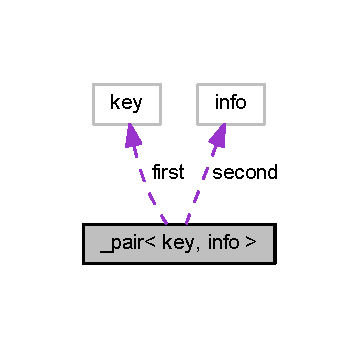
\includegraphics[width=174pt]{struct__pair__coll__graph}
\end{center}
\end{figure}
\subsection*{Public Types}
\begin{DoxyCompactItemize}
\item 
\mbox{\Hypertarget{struct__pair_a1d65c55b4a0d1045037cfaf69da62f2b}\label{struct__pair_a1d65c55b4a0d1045037cfaf69da62f2b}} 
typedef key {\bfseries \+\_\+first\+\_\+type}
\item 
\mbox{\Hypertarget{struct__pair_ab9fc2b18076a9296b20e071eb570bff9}\label{struct__pair_ab9fc2b18076a9296b20e071eb570bff9}} 
typedef info {\bfseries \+\_\+second\+\_\+type}
\end{DoxyCompactItemize}
\subsection*{Public Member Functions}
\begin{DoxyCompactItemize}
\item 
\mbox{\Hypertarget{struct__pair_a2d8582c344341d37595d71d0bd9d4c0f}\label{struct__pair_a2d8582c344341d37595d71d0bd9d4c0f}} 
{\bfseries \+\_\+pair} (const key \&t\+\_\+key, const info \&t\+\_\+info)
\item 
\mbox{\Hypertarget{struct__pair_ae2313b7dca4020743f7e36f66daa9e6c}\label{struct__pair_ae2313b7dca4020743f7e36f66daa9e6c}} 
{\bfseries \+\_\+pair} (const \mbox{\hyperlink{struct__pair}{\+\_\+pair}}$<$ key, info $>$ \&t\+\_\+pair)
\item 
\mbox{\Hypertarget{struct__pair_a53607c8d4c3e171bd27105eb763dcbdf}\label{struct__pair_a53607c8d4c3e171bd27105eb763dcbdf}} 
\mbox{\hyperlink{struct__pair}{\+\_\+pair}}$<$ key, info $>$ \& {\bfseries \+\_\+make\+\_\+pair} (const key \&t\+\_\+key, const info \&t\+\_\+info)
\item 
\mbox{\Hypertarget{struct__pair_ae459d706ae4b2dff62b65b4c3ed6fcd3}\label{struct__pair_ae459d706ae4b2dff62b65b4c3ed6fcd3}} 
\mbox{\hyperlink{struct__pair}{\+\_\+pair}}$<$ key, info $>$ \& {\bfseries operator=} (const \mbox{\hyperlink{struct__pair}{\+\_\+pair}}$<$ key, info $>$ \&t\+\_\+pair)
\item 
\mbox{\Hypertarget{struct__pair_a57a0413e35f985651dc043b5f05d14f1}\label{struct__pair_a57a0413e35f985651dc043b5f05d14f1}} 
\mbox{\hyperlink{struct__pair}{\+\_\+pair}}$<$ key, info $>$ \& {\bfseries operator=} (\mbox{\hyperlink{struct__pair}{\+\_\+pair}}$<$ key, info $>$ \&\&t\+\_\+pair)
\item 
\mbox{\Hypertarget{struct__pair_a123a7544157c973429552db3f2603433}\label{struct__pair_a123a7544157c973429552db3f2603433}} 
const \mbox{\hyperlink{struct__pair}{\+\_\+pair}}$<$ key, info $>$ \& {\bfseries operator$\ast$} ()
\item 
\mbox{\Hypertarget{struct__pair_a3704a4ada0cb96a307aacecd0993ad01}\label{struct__pair_a3704a4ada0cb96a307aacecd0993ad01}} 
const \mbox{\hyperlink{struct__pair}{\+\_\+pair}}$<$ key, info $>$ $\ast$ {\bfseries operator-\/$>$} ()
\end{DoxyCompactItemize}
\subsection*{Public Attributes}
\begin{DoxyCompactItemize}
\item 
\mbox{\Hypertarget{struct__pair_a261c3a7bc0c2157e8cc2f9a75fd6d0b9}\label{struct__pair_a261c3a7bc0c2157e8cc2f9a75fd6d0b9}} 
key {\bfseries first}
\item 
\mbox{\Hypertarget{struct__pair_a0833ec662e914d84d8bc269e57bef95a}\label{struct__pair_a0833ec662e914d84d8bc269e57bef95a}} 
info {\bfseries second}
\end{DoxyCompactItemize}


The documentation for this struct was generated from the following file\+:\begin{DoxyCompactItemize}
\item 
C\+:/\+Users/\+Sema/\+Desktop/\+Code\+Forces/\+Labs/4th\+\_\+\+Lab + library connection/\+Library/\+\_\+map.\+h\end{DoxyCompactItemize}

\hypertarget{class_aircraft_carrier_group_1_1_aircraft}{}\section{Aircraft\+Carrier\+Group\+:\+:Aircraft Class Reference}
\label{class_aircraft_carrier_group_1_1_aircraft}\index{Aircraft\+Carrier\+Group\+::\+Aircraft@{Aircraft\+Carrier\+Group\+::\+Aircraft}}


Класс для описания самолета  Осуществляет хранение всех параметров самолета и содержит функции, обрабатывающие эти параметры  




{\ttfamily \#include $<$Aircraft.\+h$>$}



Inheritance diagram for Aircraft\+Carrier\+Group\+:\+:Aircraft\+:
\nopagebreak
\begin{figure}[H]
\begin{center}
\leavevmode
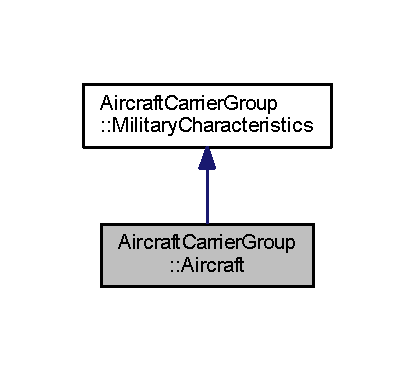
\includegraphics[width=199pt]{class_aircraft_carrier_group_1_1_aircraft__inherit__graph}
\end{center}
\end{figure}


Collaboration diagram for Aircraft\+Carrier\+Group\+:\+:Aircraft\+:
\nopagebreak
\begin{figure}[H]
\begin{center}
\leavevmode
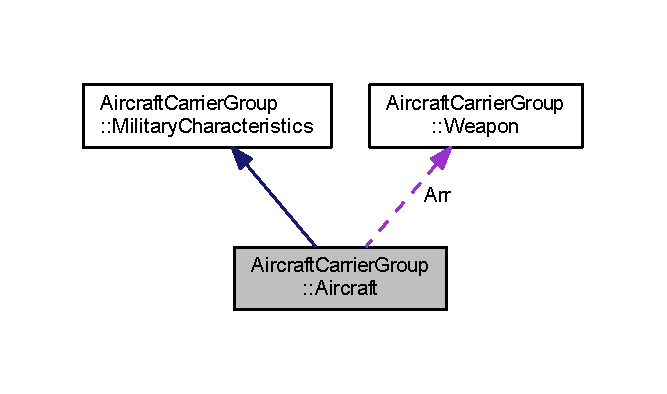
\includegraphics[width=320pt]{class_aircraft_carrier_group_1_1_aircraft__coll__graph}
\end{center}
\end{figure}
\subsection*{Public Member Functions}
\begin{DoxyCompactItemize}
\item 
\mbox{\Hypertarget{class_aircraft_carrier_group_1_1_aircraft_a5972a286b5968e4239adb81e39cdc265}\label{class_aircraft_carrier_group_1_1_aircraft_a5972a286b5968e4239adb81e39cdc265}} 
\mbox{\hyperlink{class_aircraft_carrier_group_1_1_aircraft_a5972a286b5968e4239adb81e39cdc265}{Aircraft}} ()
\begin{DoxyCompactList}\small\item\em Конструктор по умолчанию \end{DoxyCompactList}\item 
\mbox{\hyperlink{class_aircraft_carrier_group_1_1_aircraft_a4e57cd1e9950eb18c1aa4ce3b6f55c8c}{Aircraft}} (int Speed\+Tmp, int Fuel\+Reserve\+Tmp, int Fuel\+Consumption\+Tmp)
\begin{DoxyCompactList}\small\item\em Инициализирующий конструктор \end{DoxyCompactList}\item 
\mbox{\hyperlink{class_aircraft_carrier_group_1_1_aircraft_addf184db93824c8a9762101740249781}{Aircraft}} (int Speed\+Tmp, int Fuel\+Reserve\+Tmp, int Fuel\+Consumption\+Tmp, int Amount\+Tmp, \mbox{\hyperlink{class_aircraft_carrier_group_1_1_weapon}{Weapon}} $\ast$Arr\+Tmp)
\begin{DoxyCompactList}\small\item\em Инициализирующий конструктор \end{DoxyCompactList}\item 
\mbox{\hyperlink{class_aircraft_carrier_group_1_1_aircraft_a14206f9c1eadff0e4b665eeb25f9f78f}{Aircraft}} (const \mbox{\hyperlink{class_aircraft_carrier_group_1_1_military_characteristics}{Military\+Characteristics}} \&Military, int Amount\+Tmp, \mbox{\hyperlink{class_aircraft_carrier_group_1_1_weapon}{Weapon}} $\ast$Arr\+Tmp)
\begin{DoxyCompactList}\small\item\em Инициализирующий конструктор \end{DoxyCompactList}\item 
\mbox{\hyperlink{class_aircraft_carrier_group_1_1_aircraft_ad519702e8d3b7057d6345adf708a1397}{Aircraft}} (const \mbox{\hyperlink{class_aircraft_carrier_group_1_1_aircraft}{Aircraft}} \&Plane)
\begin{DoxyCompactList}\small\item\em Копирующий конструктор \end{DoxyCompactList}\item 
\mbox{\Hypertarget{class_aircraft_carrier_group_1_1_aircraft_a7df76027eeb83a2263538908c2756462}\label{class_aircraft_carrier_group_1_1_aircraft_a7df76027eeb83a2263538908c2756462}} 
\mbox{\hyperlink{class_aircraft_carrier_group_1_1_aircraft_a7df76027eeb83a2263538908c2756462}{$\sim$\+Aircraft}} ()
\begin{DoxyCompactList}\small\item\em Деструктор \end{DoxyCompactList}\item 
\mbox{\hyperlink{class_aircraft_carrier_group_1_1_weapon}{Weapon}} \& \mbox{\hyperlink{class_aircraft_carrier_group_1_1_aircraft_ae6a5bd6784855950aa8a65e3a127ebd3}{get\+Weapon\+Aircraft}} (int Number) const
\begin{DoxyCompactList}\small\item\em Возвращает описатель оружия по его номеру \end{DoxyCompactList}\item 
\mbox{\Hypertarget{class_aircraft_carrier_group_1_1_aircraft_ab60c6e2b2d91db2608b0e7ed7f6596f2}\label{class_aircraft_carrier_group_1_1_aircraft_ab60c6e2b2d91db2608b0e7ed7f6596f2}} 
int \mbox{\hyperlink{class_aircraft_carrier_group_1_1_aircraft_ab60c6e2b2d91db2608b0e7ed7f6596f2}{get\+Amount\+Weapon}} () const
\begin{DoxyCompactList}\small\item\em Возвращает количество вооружения в самолете \end{DoxyCompactList}\item 
\mbox{\Hypertarget{class_aircraft_carrier_group_1_1_aircraft_a97d17d8e918a9c949ebd3076ecdb66e6}\label{class_aircraft_carrier_group_1_1_aircraft_a97d17d8e918a9c949ebd3076ecdb66e6}} 
\mbox{\hyperlink{class_aircraft_carrier_group_1_1_aircraft}{Aircraft}} \& {\bfseries operator=} (const \mbox{\hyperlink{class_aircraft_carrier_group_1_1_aircraft}{Aircraft}} \&Plane)
\item 
\mbox{\Hypertarget{class_aircraft_carrier_group_1_1_aircraft_a754e1130fb42aaf27b9ebe4ee45a8351}\label{class_aircraft_carrier_group_1_1_aircraft_a754e1130fb42aaf27b9ebe4ee45a8351}} 
\mbox{\hyperlink{class_aircraft_carrier_group_1_1_aircraft}{Aircraft}} \& {\bfseries operator=} (\mbox{\hyperlink{class_aircraft_carrier_group_1_1_aircraft}{Aircraft}} \&\&Plane)
\item 
\mbox{\Hypertarget{class_aircraft_carrier_group_1_1_aircraft_af332f3a26edf7e69d13d928302b02159}\label{class_aircraft_carrier_group_1_1_aircraft_af332f3a26edf7e69d13d928302b02159}} 
\mbox{\hyperlink{class_aircraft_carrier_group_1_1_aircraft}{Aircraft}} $\ast$ {\bfseries operator$\ast$} ()
\end{DoxyCompactItemize}
\subsection*{Protected Attributes}
\begin{DoxyCompactItemize}
\item 
\mbox{\Hypertarget{class_aircraft_carrier_group_1_1_aircraft_af53d6b1776b3ebd20b64843b5b6d7785}\label{class_aircraft_carrier_group_1_1_aircraft_af53d6b1776b3ebd20b64843b5b6d7785}} 
int {\bfseries Amount}
\item 
\mbox{\Hypertarget{class_aircraft_carrier_group_1_1_aircraft_a4edf7fbcaf2fb3621a80ae2e92fb249e}\label{class_aircraft_carrier_group_1_1_aircraft_a4edf7fbcaf2fb3621a80ae2e92fb249e}} 
\mbox{\hyperlink{class_aircraft_carrier_group_1_1_weapon}{Weapon}} $\ast$ {\bfseries Arr}
\end{DoxyCompactItemize}
\subsection*{Static Protected Attributes}
\begin{DoxyCompactItemize}
\item 
\mbox{\Hypertarget{class_aircraft_carrier_group_1_1_aircraft_a00a4f361c3a1df31dff26d83a42c4e39}\label{class_aircraft_carrier_group_1_1_aircraft_a00a4f361c3a1df31dff26d83a42c4e39}} 
static const int {\bfseries Q\+U\+O\+TA} = 3
\end{DoxyCompactItemize}
\subsection*{Friends}
\begin{DoxyCompactItemize}
\item 
\mbox{\Hypertarget{class_aircraft_carrier_group_1_1_aircraft_a50cdd2c0cbf245722f2a454b9275bdb8}\label{class_aircraft_carrier_group_1_1_aircraft_a50cdd2c0cbf245722f2a454b9275bdb8}} 
std\+::ostream \& {\bfseries operator$<$$<$} (std\+::ostream \&os, const \mbox{\hyperlink{class_aircraft_carrier_group_1_1_aircraft}{Aircraft}} \&Plane)
\item 
\mbox{\Hypertarget{class_aircraft_carrier_group_1_1_aircraft_a8d14cc002b185ef2a06da4e01d2d9e2a}\label{class_aircraft_carrier_group_1_1_aircraft_a8d14cc002b185ef2a06da4e01d2d9e2a}} 
std\+::istream \& {\bfseries operator$>$$>$} (std\+::istream \&is, \mbox{\hyperlink{class_aircraft_carrier_group_1_1_aircraft}{Aircraft}} \&Plane)
\item 
\mbox{\Hypertarget{class_aircraft_carrier_group_1_1_aircraft_a4aca1bee1af26a984a0694c588a79d43}\label{class_aircraft_carrier_group_1_1_aircraft_a4aca1bee1af26a984a0694c588a79d43}} 
std\+::ofstream \& {\bfseries operator$<$$<$} (std\+::ofstream \&os, const \mbox{\hyperlink{class_aircraft_carrier_group_1_1_aircraft}{Aircraft}} \&Plane)
\item 
\mbox{\Hypertarget{class_aircraft_carrier_group_1_1_aircraft_a8cd1afd508ef28d2325d4dbb12eb2eff}\label{class_aircraft_carrier_group_1_1_aircraft_a8cd1afd508ef28d2325d4dbb12eb2eff}} 
std\+::ifstream \& {\bfseries operator$>$$>$} (std\+::ifstream \&is, \mbox{\hyperlink{class_aircraft_carrier_group_1_1_aircraft}{Aircraft}} \&Plane)
\end{DoxyCompactItemize}


\subsection{Detailed Description}
Класс для описания самолета  Осуществляет хранение всех параметров самолета и содержит функции, обрабатывающие эти параметры 

\subsection{Constructor \& Destructor Documentation}
\mbox{\Hypertarget{class_aircraft_carrier_group_1_1_aircraft_a4e57cd1e9950eb18c1aa4ce3b6f55c8c}\label{class_aircraft_carrier_group_1_1_aircraft_a4e57cd1e9950eb18c1aa4ce3b6f55c8c}} 
\index{Aircraft\+Carrier\+Group\+::\+Aircraft@{Aircraft\+Carrier\+Group\+::\+Aircraft}!Aircraft@{Aircraft}}
\index{Aircraft@{Aircraft}!Aircraft\+Carrier\+Group\+::\+Aircraft@{Aircraft\+Carrier\+Group\+::\+Aircraft}}
\subsubsection{\texorpdfstring{Aircraft()}{Aircraft()}\hspace{0.1cm}{\footnotesize\ttfamily [1/4]}}
{\footnotesize\ttfamily Aircraft\+Carrier\+Group\+::\+Aircraft\+::\+Aircraft (\begin{DoxyParamCaption}\item[{int}]{Speed\+Tmp,  }\item[{int}]{Fuel\+Reserve\+Tmp,  }\item[{int}]{Fuel\+Consumption\+Tmp }\end{DoxyParamCaption})\hspace{0.3cm}{\ttfamily [inline]}}



Инициализирующий конструктор 


\begin{DoxyParams}{Parameters}
{\em Speed\+Tmp} & Скорость \\
\hline
{\em Fuel\+Reserve\+Tmp} & Запас топлива \\
\hline
{\em Fuel\+Consumption\+Tmp} & Расход топлива \\
\hline
\end{DoxyParams}

\begin{DoxyExceptions}{Exceptions}
{\em Invalid\+Quota} & Если количество передаваемых орудий превышает Q\+U\+O\+TA \\
\hline
\end{DoxyExceptions}
\mbox{\Hypertarget{class_aircraft_carrier_group_1_1_aircraft_addf184db93824c8a9762101740249781}\label{class_aircraft_carrier_group_1_1_aircraft_addf184db93824c8a9762101740249781}} 
\index{Aircraft\+Carrier\+Group\+::\+Aircraft@{Aircraft\+Carrier\+Group\+::\+Aircraft}!Aircraft@{Aircraft}}
\index{Aircraft@{Aircraft}!Aircraft\+Carrier\+Group\+::\+Aircraft@{Aircraft\+Carrier\+Group\+::\+Aircraft}}
\subsubsection{\texorpdfstring{Aircraft()}{Aircraft()}\hspace{0.1cm}{\footnotesize\ttfamily [2/4]}}
{\footnotesize\ttfamily Aircraft\+Carrier\+Group\+::\+Aircraft\+::\+Aircraft (\begin{DoxyParamCaption}\item[{int}]{Speed\+Tmp,  }\item[{int}]{Fuel\+Reserve\+Tmp,  }\item[{int}]{Fuel\+Consumption\+Tmp,  }\item[{int}]{Amount\+Tmp,  }\item[{\mbox{\hyperlink{class_aircraft_carrier_group_1_1_weapon}{Weapon}} $\ast$}]{Arr\+Tmp }\end{DoxyParamCaption})}



Инициализирующий конструктор 


\begin{DoxyParams}{Parameters}
{\em Speed\+Tmp} & Скорость \\
\hline
{\em Fuel\+Reserve\+Tmp} & Запас топлива \\
\hline
{\em Fuel\+Consumption\+Tmp} & Расход топлива \\
\hline
{\em Amount\+Tmp} & Количество оружия \\
\hline
{\em Arr\+Tmp} & Массив, в котором хранится описатель каждого оружия \\
\hline
\end{DoxyParams}

\begin{DoxyExceptions}{Exceptions}
{\em Invalid\+Quota} & Если количество передаваемых орудий превышает Q\+U\+O\+TA \\
\hline
\end{DoxyExceptions}
\mbox{\Hypertarget{class_aircraft_carrier_group_1_1_aircraft_a14206f9c1eadff0e4b665eeb25f9f78f}\label{class_aircraft_carrier_group_1_1_aircraft_a14206f9c1eadff0e4b665eeb25f9f78f}} 
\index{Aircraft\+Carrier\+Group\+::\+Aircraft@{Aircraft\+Carrier\+Group\+::\+Aircraft}!Aircraft@{Aircraft}}
\index{Aircraft@{Aircraft}!Aircraft\+Carrier\+Group\+::\+Aircraft@{Aircraft\+Carrier\+Group\+::\+Aircraft}}
\subsubsection{\texorpdfstring{Aircraft()}{Aircraft()}\hspace{0.1cm}{\footnotesize\ttfamily [3/4]}}
{\footnotesize\ttfamily Aircraft\+Carrier\+Group\+::\+Aircraft\+::\+Aircraft (\begin{DoxyParamCaption}\item[{const \mbox{\hyperlink{class_aircraft_carrier_group_1_1_military_characteristics}{Military\+Characteristics}} \&}]{Military,  }\item[{int}]{Amount\+Tmp = {\ttfamily 0},  }\item[{\mbox{\hyperlink{class_aircraft_carrier_group_1_1_weapon}{Weapon}} $\ast$}]{Arr\+Tmp = {\ttfamily nullptr} }\end{DoxyParamCaption})}



Инициализирующий конструктор 


\begin{DoxyParams}{Parameters}
{\em Military} & Хранит общие характеристики техники \\
\hline
{\em Amount\+Tmp} & Количество вооружения \\
\hline
{\em Arr\+Tmp} & Массив, в котором хрнаится описатель каждого оружия \\
\hline
\end{DoxyParams}

\begin{DoxyExceptions}{Exceptions}
{\em Invalid\+Quota} & Если количество передаваемых орудий превышает Q\+U\+O\+TA \\
\hline
\end{DoxyExceptions}
\mbox{\Hypertarget{class_aircraft_carrier_group_1_1_aircraft_ad519702e8d3b7057d6345adf708a1397}\label{class_aircraft_carrier_group_1_1_aircraft_ad519702e8d3b7057d6345adf708a1397}} 
\index{Aircraft\+Carrier\+Group\+::\+Aircraft@{Aircraft\+Carrier\+Group\+::\+Aircraft}!Aircraft@{Aircraft}}
\index{Aircraft@{Aircraft}!Aircraft\+Carrier\+Group\+::\+Aircraft@{Aircraft\+Carrier\+Group\+::\+Aircraft}}
\subsubsection{\texorpdfstring{Aircraft()}{Aircraft()}\hspace{0.1cm}{\footnotesize\ttfamily [4/4]}}
{\footnotesize\ttfamily Aircraft\+Carrier\+Group\+::\+Aircraft\+::\+Aircraft (\begin{DoxyParamCaption}\item[{const \mbox{\hyperlink{class_aircraft_carrier_group_1_1_aircraft}{Aircraft}} \&}]{Plane }\end{DoxyParamCaption})}



Копирующий конструктор 


\begin{DoxyParams}{Parameters}
{\em Plane} & Описатель самолета \\
\hline
\end{DoxyParams}


\subsection{Member Function Documentation}
\mbox{\Hypertarget{class_aircraft_carrier_group_1_1_aircraft_ae6a5bd6784855950aa8a65e3a127ebd3}\label{class_aircraft_carrier_group_1_1_aircraft_ae6a5bd6784855950aa8a65e3a127ebd3}} 
\index{Aircraft\+Carrier\+Group\+::\+Aircraft@{Aircraft\+Carrier\+Group\+::\+Aircraft}!get\+Weapon\+Aircraft@{get\+Weapon\+Aircraft}}
\index{get\+Weapon\+Aircraft@{get\+Weapon\+Aircraft}!Aircraft\+Carrier\+Group\+::\+Aircraft@{Aircraft\+Carrier\+Group\+::\+Aircraft}}
\subsubsection{\texorpdfstring{get\+Weapon\+Aircraft()}{getWeaponAircraft()}}
{\footnotesize\ttfamily \mbox{\hyperlink{class_aircraft_carrier_group_1_1_weapon}{Weapon}} \& Aircraft\+Carrier\+Group\+::\+Aircraft\+::get\+Weapon\+Aircraft (\begin{DoxyParamCaption}\item[{int}]{Number }\end{DoxyParamCaption}) const}



Возвращает описатель оружия по его номеру 


\begin{DoxyParams}{Parameters}
{\em Number} & Номер оружия \\
\hline
\end{DoxyParams}

\begin{DoxyExceptions}{Exceptions}
{\em Invalid\+Number\+Weapon} & Есди был задан неверный номер оружия \\
\hline
\end{DoxyExceptions}


The documentation for this class was generated from the following files\+:\begin{DoxyCompactItemize}
\item 
C\+:/\+Users/\+Sema/\+Desktop/\+Code\+Forces/\+Labs/4th\+\_\+\+Lab + library connection/\+Library/\mbox{\hyperlink{_aircraft_8h}{Aircraft.\+h}}\item 
C\+:/\+Users/\+Sema/\+Desktop/\+Code\+Forces/\+Labs/4th\+\_\+\+Lab + library connection/\+Library/Aircraft.\+cpp\end{DoxyCompactItemize}

\hypertarget{class_aircraft_carrier_group_1_1_aircraft_carrier}{}\section{Aircraft\+Carrier\+Group\+:\+:Aircraft\+Carrier Class Reference}
\label{class_aircraft_carrier_group_1_1_aircraft_carrier}\index{Aircraft\+Carrier\+Group\+::\+Aircraft\+Carrier@{Aircraft\+Carrier\+Group\+::\+Aircraft\+Carrier}}


Класс для описания авианесущего крейсера  Осуществляет хранение всех параметров авианесущего крейсера и содержит функции, обрабатывающие эти параметры  




{\ttfamily \#include $<$Aircraft\+Carrier.\+h$>$}



Inheritance diagram for Aircraft\+Carrier\+Group\+:\+:Aircraft\+Carrier\+:
\nopagebreak
\begin{figure}[H]
\begin{center}
\leavevmode
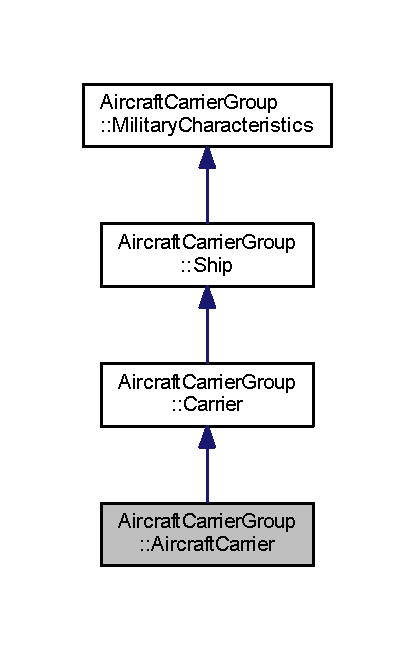
\includegraphics[width=199pt]{class_aircraft_carrier_group_1_1_aircraft_carrier__inherit__graph}
\end{center}
\end{figure}


Collaboration diagram for Aircraft\+Carrier\+Group\+:\+:Aircraft\+Carrier\+:
\nopagebreak
\begin{figure}[H]
\begin{center}
\leavevmode
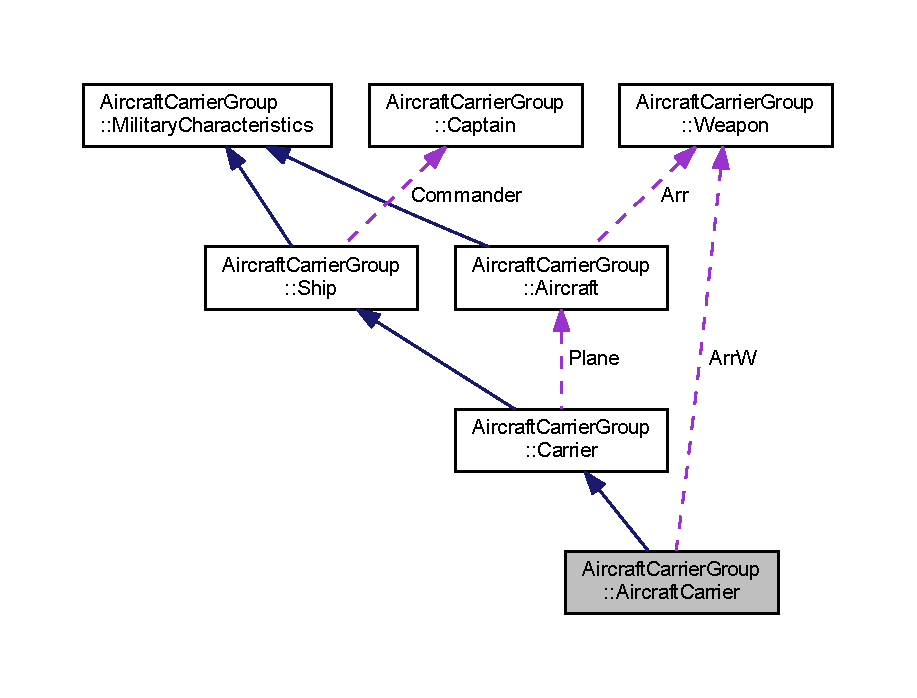
\includegraphics[width=350pt]{class_aircraft_carrier_group_1_1_aircraft_carrier__coll__graph}
\end{center}
\end{figure}
\subsection*{Public Member Functions}
\begin{DoxyCompactItemize}
\item 
\mbox{\Hypertarget{class_aircraft_carrier_group_1_1_aircraft_carrier_a0eca59a4e28727be647e108a02feccb6}\label{class_aircraft_carrier_group_1_1_aircraft_carrier_a0eca59a4e28727be647e108a02feccb6}} 
\mbox{\hyperlink{class_aircraft_carrier_group_1_1_aircraft_carrier_a0eca59a4e28727be647e108a02feccb6}{Aircraft\+Carrier}} ()
\begin{DoxyCompactList}\small\item\em Конструктор по умолчанию \end{DoxyCompactList}\item 
\mbox{\hyperlink{class_aircraft_carrier_group_1_1_aircraft_carrier_a612d60f0e6c3b14158ab3b6efb63c7d5}{Aircraft\+Carrier}} (std\+::string Call\+Tmp, const \mbox{\hyperlink{struct_aircraft_carrier_group_1_1_captain}{Captain}} \&Commander\+Tmp, int Crew\+Tmp, const \mbox{\hyperlink{class_aircraft_carrier_group_1_1_military_characteristics}{Military\+Characteristics}} \&Military\+Tmp, int Amount\+P\+Tmp, \mbox{\hyperlink{class_aircraft_carrier_group_1_1_aircraft}{Aircraft}} $\ast$Plane\+Tmp, int Amount\+W\+Tmp, \mbox{\hyperlink{class_aircraft_carrier_group_1_1_weapon}{Weapon}} $\ast$Arr\+W\+Tmp)
\begin{DoxyCompactList}\small\item\em Инициализирующий конструктор \end{DoxyCompactList}\item 
\mbox{\hyperlink{class_aircraft_carrier_group_1_1_aircraft_carrier_a06e80069d3a9240871e6af9018cec8b9}{Aircraft\+Carrier}} (const \mbox{\hyperlink{class_aircraft_carrier_group_1_1_aircraft_carrier}{Aircraft\+Carrier}} \&Aerocarrier\+Tmp)
\begin{DoxyCompactList}\small\item\em Копирующий конструктор \end{DoxyCompactList}\item 
\mbox{\Hypertarget{class_aircraft_carrier_group_1_1_aircraft_carrier_ace72f0b7cd3dc96d95652233f3aec670}\label{class_aircraft_carrier_group_1_1_aircraft_carrier_ace72f0b7cd3dc96d95652233f3aec670}} 
\mbox{\hyperlink{class_aircraft_carrier_group_1_1_aircraft_carrier_ace72f0b7cd3dc96d95652233f3aec670}{$\sim$\+Aircraft\+Carrier}} ()
\begin{DoxyCompactList}\small\item\em Деструктор \end{DoxyCompactList}\item 
\mbox{\Hypertarget{class_aircraft_carrier_group_1_1_aircraft_carrier_a7ca6cefb553d9f6c0b62874f6bf7ec95}\label{class_aircraft_carrier_group_1_1_aircraft_carrier_a7ca6cefb553d9f6c0b62874f6bf7ec95}} 
std\+::ostream \& \mbox{\hyperlink{class_aircraft_carrier_group_1_1_aircraft_carrier_a7ca6cefb553d9f6c0b62874f6bf7ec95}{print\+Info\+Weapon}} (std\+::ostream \&os) const
\begin{DoxyCompactList}\small\item\em Выводит всю информацию обо всех орудиях на судне \end{DoxyCompactList}\item 
\mbox{\Hypertarget{class_aircraft_carrier_group_1_1_aircraft_carrier_ab2caba5f25f136dff2354539b47ff68c}\label{class_aircraft_carrier_group_1_1_aircraft_carrier_ab2caba5f25f136dff2354539b47ff68c}} 
int \mbox{\hyperlink{class_aircraft_carrier_group_1_1_aircraft_carrier_ab2caba5f25f136dff2354539b47ff68c}{Damage\+All\+Weapons}} () const
\begin{DoxyCompactList}\small\item\em Производит расчет разрушений, которые могут нанести все орудия судна условной цели за единицу времени \end{DoxyCompactList}\item 
\mbox{\Hypertarget{class_aircraft_carrier_group_1_1_aircraft_carrier_a6613d24d38f7a28d20f35437bc069f98}\label{class_aircraft_carrier_group_1_1_aircraft_carrier_a6613d24d38f7a28d20f35437bc069f98}} 
double \mbox{\hyperlink{class_aircraft_carrier_group_1_1_aircraft_carrier_a6613d24d38f7a28d20f35437bc069f98}{Time\+Fire\+All\+Weapons}} () const
\begin{DoxyCompactList}\small\item\em Производит рассчет времени ведения огня всеми орудиями судна с полной скорострельностью \end{DoxyCompactList}\item 
\mbox{\hyperlink{class_aircraft_carrier_group_1_1_aircraft_carrier}{Aircraft\+Carrier}} \& \mbox{\hyperlink{class_aircraft_carrier_group_1_1_aircraft_carrier_a36f838dfc52ea713a12ab74a2ebe237d}{Weapon\+Modification}} (std\+::string Name\+Weapon\+Tmp, \mbox{\hyperlink{class_aircraft_carrier_group_1_1_weapon}{Weapon}} \&Weapon\+Tmp)
\begin{DoxyCompactList}\small\item\em Функция модифицирует выбранное, из имеющихся на корабле, орудие \end{DoxyCompactList}\item 
\mbox{\hyperlink{class_aircraft_carrier_group_1_1_aircraft_carrier}{Aircraft\+Carrier}} $\ast$ \mbox{\hyperlink{class_aircraft_carrier_group_1_1_aircraft_carrier_ab2f921c586a31f9933874f437baf9c16}{clone}} () const
\begin{DoxyCompactList}\small\item\em Клонирует данный корабль \end{DoxyCompactList}\item 
\mbox{\hyperlink{class_aircraft_carrier_group_1_1_weapon}{Weapon}} $\ast$ \mbox{\hyperlink{class_aircraft_carrier_group_1_1_aircraft_carrier_aa7839178084e4f749592e02d2d8e93a4}{get\+Weapon}} (std\+::string Name) const
\begin{DoxyCompactList}\small\item\em Функция получает описатель оружия по его названию \end{DoxyCompactList}\item 
\mbox{\Hypertarget{class_aircraft_carrier_group_1_1_aircraft_carrier_abddfdb193451143aa371c5fb86705afb}\label{class_aircraft_carrier_group_1_1_aircraft_carrier_abddfdb193451143aa371c5fb86705afb}} 
int \mbox{\hyperlink{class_aircraft_carrier_group_1_1_aircraft_carrier_abddfdb193451143aa371c5fb86705afb}{Amount\+Weapon}} () const
\begin{DoxyCompactList}\small\item\em Возвращает количество вооружения на судне \end{DoxyCompactList}\item 
\mbox{\Hypertarget{class_aircraft_carrier_group_1_1_aircraft_carrier_a23197fb96cb38227da69687d8fe75124}\label{class_aircraft_carrier_group_1_1_aircraft_carrier_a23197fb96cb38227da69687d8fe75124}} 
int \mbox{\hyperlink{class_aircraft_carrier_group_1_1_aircraft_carrier_a23197fb96cb38227da69687d8fe75124}{Type\+Ship}} () const
\begin{DoxyCompactList}\small\item\em Тип данного корабля \end{DoxyCompactList}\item 
std\+::string \mbox{\hyperlink{class_aircraft_carrier_group_1_1_aircraft_carrier_ae6d7a76049249ef218e6859334ed2eaa}{Get\+Disguised}} () const
\begin{DoxyCompactList}\small\item\em Функция возвращет названия прикрываемого корабля \end{DoxyCompactList}\end{DoxyCompactItemize}
\subsection*{Protected Member Functions}
\begin{DoxyCompactItemize}
\item 
\mbox{\Hypertarget{class_aircraft_carrier_group_1_1_aircraft_carrier_a5d956c0217b7393e829e85caea6fb1fe}\label{class_aircraft_carrier_group_1_1_aircraft_carrier_a5d956c0217b7393e829e85caea6fb1fe}} 
virtual std\+::ostream \& {\bfseries show} (std\+::ostream \&os) const
\item 
\mbox{\Hypertarget{class_aircraft_carrier_group_1_1_aircraft_carrier_a1bbf12101788a88387a7e76e6aa1e6b4}\label{class_aircraft_carrier_group_1_1_aircraft_carrier_a1bbf12101788a88387a7e76e6aa1e6b4}} 
virtual std\+::istream \& {\bfseries get} (std\+::istream \&)
\item 
\mbox{\Hypertarget{class_aircraft_carrier_group_1_1_aircraft_carrier_a27d2e7f4970d513df2c50181c59921d1}\label{class_aircraft_carrier_group_1_1_aircraft_carrier_a27d2e7f4970d513df2c50181c59921d1}} 
virtual std\+::ofstream \& {\bfseries fprint} (std\+::ofstream \&) const
\item 
\mbox{\Hypertarget{class_aircraft_carrier_group_1_1_aircraft_carrier_a75f2144ae0faeda9cb7d9df10ff38487}\label{class_aircraft_carrier_group_1_1_aircraft_carrier_a75f2144ae0faeda9cb7d9df10ff38487}} 
virtual std\+::ifstream \& {\bfseries fread} (std\+::ifstream \&)
\end{DoxyCompactItemize}
\subsection*{Protected Attributes}
\begin{DoxyCompactItemize}
\item 
\mbox{\Hypertarget{class_aircraft_carrier_group_1_1_aircraft_carrier_a62dd633d643f869452c86196f739fa9a}\label{class_aircraft_carrier_group_1_1_aircraft_carrier_a62dd633d643f869452c86196f739fa9a}} 
int {\bfseries AmountW}
\item 
\mbox{\Hypertarget{class_aircraft_carrier_group_1_1_aircraft_carrier_a1922eb4020301c80903d841a65df1b92}\label{class_aircraft_carrier_group_1_1_aircraft_carrier_a1922eb4020301c80903d841a65df1b92}} 
\mbox{\hyperlink{class_aircraft_carrier_group_1_1_weapon}{Weapon}} $\ast$ {\bfseries ArrW}
\end{DoxyCompactItemize}
\subsection*{Friends}
\begin{DoxyCompactItemize}
\item 
\mbox{\Hypertarget{class_aircraft_carrier_group_1_1_aircraft_carrier_aceadecaaab410111d76743b193972651}\label{class_aircraft_carrier_group_1_1_aircraft_carrier_aceadecaaab410111d76743b193972651}} 
std\+::ostream \& {\bfseries operator$<$$<$} (std\+::ostream \&, const \mbox{\hyperlink{class_aircraft_carrier_group_1_1_aircraft_carrier}{Aircraft\+Carrier}} \&)
\item 
\mbox{\Hypertarget{class_aircraft_carrier_group_1_1_aircraft_carrier_a9a3a3c478af09b6941e89c0fefcb73b9}\label{class_aircraft_carrier_group_1_1_aircraft_carrier_a9a3a3c478af09b6941e89c0fefcb73b9}} 
std\+::istream \& {\bfseries operator$>$$>$} (std\+::istream \&, \mbox{\hyperlink{class_aircraft_carrier_group_1_1_aircraft_carrier}{Aircraft\+Carrier}} \&)
\item 
\mbox{\Hypertarget{class_aircraft_carrier_group_1_1_aircraft_carrier_adb7d0edf5f6031c0fcee267e02f38528}\label{class_aircraft_carrier_group_1_1_aircraft_carrier_adb7d0edf5f6031c0fcee267e02f38528}} 
std\+::ofstream \& {\bfseries operator$<$$<$} (std\+::ofstream \&os, const \mbox{\hyperlink{class_aircraft_carrier_group_1_1_aircraft_carrier}{Aircraft\+Carrier}} \&Ship\+Tmp)
\item 
\mbox{\Hypertarget{class_aircraft_carrier_group_1_1_aircraft_carrier_a45f3e10b1bd4a3af9457a15d034e60ad}\label{class_aircraft_carrier_group_1_1_aircraft_carrier_a45f3e10b1bd4a3af9457a15d034e60ad}} 
std\+::ifstream \& {\bfseries operator$>$$>$} (std\+::ifstream \&is, \mbox{\hyperlink{class_aircraft_carrier_group_1_1_aircraft_carrier}{Aircraft\+Carrier}} \&Ship\+Tmp)
\end{DoxyCompactItemize}


\subsection{Detailed Description}
Класс для описания авианесущего крейсера  Осуществляет хранение всех параметров авианесущего крейсера и содержит функции, обрабатывающие эти параметры 

\subsection{Constructor \& Destructor Documentation}
\mbox{\Hypertarget{class_aircraft_carrier_group_1_1_aircraft_carrier_a612d60f0e6c3b14158ab3b6efb63c7d5}\label{class_aircraft_carrier_group_1_1_aircraft_carrier_a612d60f0e6c3b14158ab3b6efb63c7d5}} 
\index{Aircraft\+Carrier\+Group\+::\+Aircraft\+Carrier@{Aircraft\+Carrier\+Group\+::\+Aircraft\+Carrier}!Aircraft\+Carrier@{Aircraft\+Carrier}}
\index{Aircraft\+Carrier@{Aircraft\+Carrier}!Aircraft\+Carrier\+Group\+::\+Aircraft\+Carrier@{Aircraft\+Carrier\+Group\+::\+Aircraft\+Carrier}}
\subsubsection{\texorpdfstring{Aircraft\+Carrier()}{AircraftCarrier()}\hspace{0.1cm}{\footnotesize\ttfamily [1/2]}}
{\footnotesize\ttfamily Aircraft\+Carrier\+Group\+::\+Aircraft\+Carrier\+::\+Aircraft\+Carrier (\begin{DoxyParamCaption}\item[{std\+::string}]{Call\+Tmp,  }\item[{const \mbox{\hyperlink{struct_aircraft_carrier_group_1_1_captain}{Captain}} \&}]{Commander\+Tmp,  }\item[{int}]{Crew\+Tmp,  }\item[{const \mbox{\hyperlink{class_aircraft_carrier_group_1_1_military_characteristics}{Military\+Characteristics}} \&}]{Military\+Tmp,  }\item[{int}]{Amount\+P\+Tmp,  }\item[{\mbox{\hyperlink{class_aircraft_carrier_group_1_1_aircraft}{Aircraft}} $\ast$}]{Plane\+Tmp,  }\item[{int}]{Amount\+W\+Tmp,  }\item[{\mbox{\hyperlink{class_aircraft_carrier_group_1_1_weapon}{Weapon}} $\ast$}]{Arr\+W\+Tmp }\end{DoxyParamCaption})}



Инициализирующий конструктор 


\begin{DoxyParams}{Parameters}
{\em Call\+Tmp} & Название корабля \\
\hline
{\em Comander\+Tmp} & Капитан судна \\
\hline
{\em Crew\+Tmp} & Количество человек в команде \\
\hline
{\em Military\+Tmp} & Хранит общие характеристики техники \\
\hline
{\em Amount\+P\+Tmp} & Количество самолетов на палубе корабля \\
\hline
{\em Plane\+Tmp} & Содержит описатели каждого из самолетов \\
\hline
{\em Amount\+W\+Tmp} & Количество вооружения на корабле \\
\hline
{\em Arr\+W\+Tmp} & Хранит описатели каждого оружия на корабле \\
\hline
\end{DoxyParams}
\mbox{\Hypertarget{class_aircraft_carrier_group_1_1_aircraft_carrier_a06e80069d3a9240871e6af9018cec8b9}\label{class_aircraft_carrier_group_1_1_aircraft_carrier_a06e80069d3a9240871e6af9018cec8b9}} 
\index{Aircraft\+Carrier\+Group\+::\+Aircraft\+Carrier@{Aircraft\+Carrier\+Group\+::\+Aircraft\+Carrier}!Aircraft\+Carrier@{Aircraft\+Carrier}}
\index{Aircraft\+Carrier@{Aircraft\+Carrier}!Aircraft\+Carrier\+Group\+::\+Aircraft\+Carrier@{Aircraft\+Carrier\+Group\+::\+Aircraft\+Carrier}}
\subsubsection{\texorpdfstring{Aircraft\+Carrier()}{AircraftCarrier()}\hspace{0.1cm}{\footnotesize\ttfamily [2/2]}}
{\footnotesize\ttfamily Aircraft\+Carrier\+Group\+::\+Aircraft\+Carrier\+::\+Aircraft\+Carrier (\begin{DoxyParamCaption}\item[{const \mbox{\hyperlink{class_aircraft_carrier_group_1_1_aircraft_carrier}{Aircraft\+Carrier}} \&}]{Aerocarrier\+Tmp }\end{DoxyParamCaption})}



Копирующий конструктор 


\begin{DoxyParams}{Parameters}
{\em Aerocarrier\+Tmp} & Описатель авианесущего крейсера \\
\hline
\end{DoxyParams}


\subsection{Member Function Documentation}
\mbox{\Hypertarget{class_aircraft_carrier_group_1_1_aircraft_carrier_ab2f921c586a31f9933874f437baf9c16}\label{class_aircraft_carrier_group_1_1_aircraft_carrier_ab2f921c586a31f9933874f437baf9c16}} 
\index{Aircraft\+Carrier\+Group\+::\+Aircraft\+Carrier@{Aircraft\+Carrier\+Group\+::\+Aircraft\+Carrier}!clone@{clone}}
\index{clone@{clone}!Aircraft\+Carrier\+Group\+::\+Aircraft\+Carrier@{Aircraft\+Carrier\+Group\+::\+Aircraft\+Carrier}}
\subsubsection{\texorpdfstring{clone()}{clone()}}
{\footnotesize\ttfamily \mbox{\hyperlink{class_aircraft_carrier_group_1_1_aircraft_carrier}{Aircraft\+Carrier}}$\ast$ Aircraft\+Carrier\+Group\+::\+Aircraft\+Carrier\+::clone (\begin{DoxyParamCaption}{ }\end{DoxyParamCaption}) const\hspace{0.3cm}{\ttfamily [inline]}, {\ttfamily [virtual]}}



Клонирует данный корабль 

\begin{DoxyReturn}{Returns}
Возвращает указатель на область памяти, в котором хранится копия этого корабля 
\end{DoxyReturn}


Reimplemented from \mbox{\hyperlink{class_aircraft_carrier_group_1_1_carrier_acb567d5ef451d10187f46c34653626e1}{Aircraft\+Carrier\+Group\+::\+Carrier}}.

Here is the call graph for this function\+:
\nopagebreak
\begin{figure}[H]
\begin{center}
\leavevmode
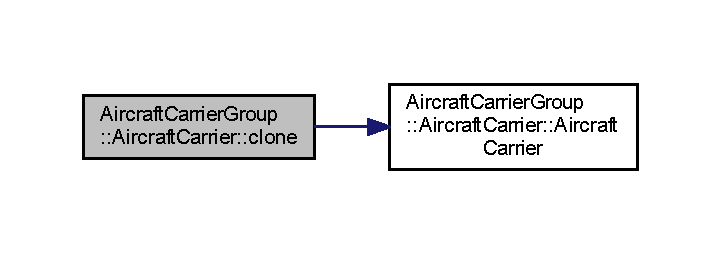
\includegraphics[width=346pt]{class_aircraft_carrier_group_1_1_aircraft_carrier_ab2f921c586a31f9933874f437baf9c16_cgraph}
\end{center}
\end{figure}
\mbox{\Hypertarget{class_aircraft_carrier_group_1_1_aircraft_carrier_ae6d7a76049249ef218e6859334ed2eaa}\label{class_aircraft_carrier_group_1_1_aircraft_carrier_ae6d7a76049249ef218e6859334ed2eaa}} 
\index{Aircraft\+Carrier\+Group\+::\+Aircraft\+Carrier@{Aircraft\+Carrier\+Group\+::\+Aircraft\+Carrier}!Get\+Disguised@{Get\+Disguised}}
\index{Get\+Disguised@{Get\+Disguised}!Aircraft\+Carrier\+Group\+::\+Aircraft\+Carrier@{Aircraft\+Carrier\+Group\+::\+Aircraft\+Carrier}}
\subsubsection{\texorpdfstring{Get\+Disguised()}{GetDisguised()}}
{\footnotesize\ttfamily std\+::string Aircraft\+Carrier\+Group\+::\+Aircraft\+Carrier\+::\+Get\+Disguised (\begin{DoxyParamCaption}{ }\end{DoxyParamCaption}) const\hspace{0.3cm}{\ttfamily [inline]}, {\ttfamily [virtual]}}



Функция возвращет названия прикрываемого корабля 


\begin{DoxyExceptions}{Exceptions}
{\em Invalid\+Ship\+Type} & При попытке получить названия прикрываемого корабля, поскольку этот тип кораблей не может иметь прикрываемого корабля \\
\hline
\end{DoxyExceptions}


Implements \mbox{\hyperlink{class_aircraft_carrier_group_1_1_ship_a6455eb63c95dd3598b45b92e42e7f84d}{Aircraft\+Carrier\+Group\+::\+Ship}}.

\mbox{\Hypertarget{class_aircraft_carrier_group_1_1_aircraft_carrier_aa7839178084e4f749592e02d2d8e93a4}\label{class_aircraft_carrier_group_1_1_aircraft_carrier_aa7839178084e4f749592e02d2d8e93a4}} 
\index{Aircraft\+Carrier\+Group\+::\+Aircraft\+Carrier@{Aircraft\+Carrier\+Group\+::\+Aircraft\+Carrier}!get\+Weapon@{get\+Weapon}}
\index{get\+Weapon@{get\+Weapon}!Aircraft\+Carrier\+Group\+::\+Aircraft\+Carrier@{Aircraft\+Carrier\+Group\+::\+Aircraft\+Carrier}}
\subsubsection{\texorpdfstring{get\+Weapon()}{getWeapon()}}
{\footnotesize\ttfamily \mbox{\hyperlink{class_aircraft_carrier_group_1_1_weapon}{Weapon}} $\ast$ Aircraft\+Carrier\+Group\+::\+Aircraft\+Carrier\+::get\+Weapon (\begin{DoxyParamCaption}\item[{std\+::string}]{Name }\end{DoxyParamCaption}) const\hspace{0.3cm}{\ttfamily [virtual]}}



Функция получает описатель оружия по его названию 


\begin{DoxyParams}{Parameters}
{\em Name} & Название оружия \\
\hline
\end{DoxyParams}
\begin{DoxyReturn}{Returns}
Возвращает указатель на область памяти, в котором хранится описатель найденного оружия 
\end{DoxyReturn}


Reimplemented from \mbox{\hyperlink{class_aircraft_carrier_group_1_1_carrier_a69e4672d2e5b0e7ff0d27e9ec762b828}{Aircraft\+Carrier\+Group\+::\+Carrier}}.

\mbox{\Hypertarget{class_aircraft_carrier_group_1_1_aircraft_carrier_a36f838dfc52ea713a12ab74a2ebe237d}\label{class_aircraft_carrier_group_1_1_aircraft_carrier_a36f838dfc52ea713a12ab74a2ebe237d}} 
\index{Aircraft\+Carrier\+Group\+::\+Aircraft\+Carrier@{Aircraft\+Carrier\+Group\+::\+Aircraft\+Carrier}!Weapon\+Modification@{Weapon\+Modification}}
\index{Weapon\+Modification@{Weapon\+Modification}!Aircraft\+Carrier\+Group\+::\+Aircraft\+Carrier@{Aircraft\+Carrier\+Group\+::\+Aircraft\+Carrier}}
\subsubsection{\texorpdfstring{Weapon\+Modification()}{WeaponModification()}}
{\footnotesize\ttfamily \mbox{\hyperlink{class_aircraft_carrier_group_1_1_aircraft_carrier}{Aircraft\+Carrier}} \& Aircraft\+Carrier\+Group\+::\+Aircraft\+Carrier\+::\+Weapon\+Modification (\begin{DoxyParamCaption}\item[{std\+::string}]{Name\+Weapon\+Tmp,  }\item[{\mbox{\hyperlink{class_aircraft_carrier_group_1_1_weapon}{Weapon}} \&}]{Weapon\+Tmp }\end{DoxyParamCaption})}



Функция модифицирует выбранное, из имеющихся на корабле, орудие 


\begin{DoxyParams}{Parameters}
{\em Name\+Weapon\+Tmp} & Названия орудия, которое надо модифицировать \\
\hline
{\em Weapon\+Tmp} & Новое орудие \\
\hline
\end{DoxyParams}


The documentation for this class was generated from the following files\+:\begin{DoxyCompactItemize}
\item 
C\+:/\+Users/\+Sema/\+Desktop/\+Code\+Forces/\+Labs/4th\+\_\+\+Lab + library connection/\+Library/\mbox{\hyperlink{_aircraft_carrier_8h}{Aircraft\+Carrier.\+h}}\item 
C\+:/\+Users/\+Sema/\+Desktop/\+Code\+Forces/\+Labs/4th\+\_\+\+Lab + library connection/\+Library/Aircraft\+Carrier.\+cpp\end{DoxyCompactItemize}

\hypertarget{struct_aircraft_carrier_group_1_1_captain}{}\section{Aircraft\+Carrier\+Group\+:\+:Captain Struct Reference}
\label{struct_aircraft_carrier_group_1_1_captain}\index{Aircraft\+Carrier\+Group\+::\+Captain@{Aircraft\+Carrier\+Group\+::\+Captain}}


Структура для описания капитана  Осуществляет хранение всех параметров командира судна или флота  




{\ttfamily \#include $<$Ship.\+h$>$}

\subsection*{Public Member Functions}
\begin{DoxyCompactItemize}
\item 
\mbox{\Hypertarget{struct_aircraft_carrier_group_1_1_captain_a6be7a710b2a305ce8670e834bf138102}\label{struct_aircraft_carrier_group_1_1_captain_a6be7a710b2a305ce8670e834bf138102}} 
\mbox{\hyperlink{struct_aircraft_carrier_group_1_1_captain_a6be7a710b2a305ce8670e834bf138102}{Captain}} ()
\begin{DoxyCompactList}\small\item\em Конструктор по умолчанию \end{DoxyCompactList}\item 
\mbox{\hyperlink{struct_aircraft_carrier_group_1_1_captain_aa9c0ef2175bb1bc073f96ae0cf8094a1}{Captain}} (std\+::string Name\+Tmp, std\+::string Rank\+Tmp, int Experience\+Tmp)
\begin{DoxyCompactList}\small\item\em Инициализирующий конструктор \end{DoxyCompactList}\item 
\mbox{\hyperlink{struct_aircraft_carrier_group_1_1_captain_a52f1e94e696b2ac771c74f6c684f6a22}{Captain}} (const \mbox{\hyperlink{struct_aircraft_carrier_group_1_1_captain}{Captain}} \&Commander\+Tmp)
\begin{DoxyCompactList}\small\item\em Копирующий конструктор \end{DoxyCompactList}\item 
\mbox{\Hypertarget{struct_aircraft_carrier_group_1_1_captain_a5729193b600c718a41ac57180fd8d61f}\label{struct_aircraft_carrier_group_1_1_captain_a5729193b600c718a41ac57180fd8d61f}} 
\mbox{\hyperlink{struct_aircraft_carrier_group_1_1_captain_a5729193b600c718a41ac57180fd8d61f}{$\sim$\+Captain}} ()
\begin{DoxyCompactList}\small\item\em Деструктор \end{DoxyCompactList}\item 
\mbox{\Hypertarget{struct_aircraft_carrier_group_1_1_captain_af9a3be6c6d93cdbbcd8297f324ecfd00}\label{struct_aircraft_carrier_group_1_1_captain_af9a3be6c6d93cdbbcd8297f324ecfd00}} 
\mbox{\hyperlink{struct_aircraft_carrier_group_1_1_captain}{Captain}} \& {\bfseries operator=} (const \mbox{\hyperlink{struct_aircraft_carrier_group_1_1_captain}{Captain}} \&)
\item 
\mbox{\Hypertarget{struct_aircraft_carrier_group_1_1_captain_aad6dbdeaadb51d01d4cf28a20c345ada}\label{struct_aircraft_carrier_group_1_1_captain_aad6dbdeaadb51d01d4cf28a20c345ada}} 
\mbox{\hyperlink{struct_aircraft_carrier_group_1_1_captain}{Captain}} \& {\bfseries operator=} (\mbox{\hyperlink{struct_aircraft_carrier_group_1_1_captain}{Captain}} \&\&)
\end{DoxyCompactItemize}
\subsection*{Public Attributes}
\begin{DoxyCompactItemize}
\item 
\mbox{\Hypertarget{struct_aircraft_carrier_group_1_1_captain_a978fb4171ae9db5a98cfe21dd8e03425}\label{struct_aircraft_carrier_group_1_1_captain_a978fb4171ae9db5a98cfe21dd8e03425}} 
std\+::string {\bfseries Name}
\item 
\mbox{\Hypertarget{struct_aircraft_carrier_group_1_1_captain_af09effcfd568475fde2fcf2e3c55cb1f}\label{struct_aircraft_carrier_group_1_1_captain_af09effcfd568475fde2fcf2e3c55cb1f}} 
std\+::string {\bfseries Rank}
\item 
\mbox{\Hypertarget{struct_aircraft_carrier_group_1_1_captain_a10365f6ea96d64ebd34649f1c9656902}\label{struct_aircraft_carrier_group_1_1_captain_a10365f6ea96d64ebd34649f1c9656902}} 
int {\bfseries Experience}
\end{DoxyCompactItemize}
\subsection*{Friends}
\begin{DoxyCompactItemize}
\item 
\mbox{\Hypertarget{struct_aircraft_carrier_group_1_1_captain_a276745bd693dc7b587811f496c7f100b}\label{struct_aircraft_carrier_group_1_1_captain_a276745bd693dc7b587811f496c7f100b}} 
std\+::istream \& {\bfseries operator$>$$>$} (std\+::istream \&is, \mbox{\hyperlink{struct_aircraft_carrier_group_1_1_captain}{Captain}} \&Commander)
\item 
\mbox{\Hypertarget{struct_aircraft_carrier_group_1_1_captain_a3d5328753431802e2ddd6be9468138a6}\label{struct_aircraft_carrier_group_1_1_captain_a3d5328753431802e2ddd6be9468138a6}} 
std\+::ostream \& {\bfseries operator$<$$<$} (std\+::ostream \&os, const \mbox{\hyperlink{struct_aircraft_carrier_group_1_1_captain}{Captain}} \&Commander)
\item 
\mbox{\Hypertarget{struct_aircraft_carrier_group_1_1_captain_af4bdd39ebe7d66247cbf7026a3c215ba}\label{struct_aircraft_carrier_group_1_1_captain_af4bdd39ebe7d66247cbf7026a3c215ba}} 
std\+::ifstream \& {\bfseries operator$>$$>$} (std\+::ifstream \&is, \mbox{\hyperlink{struct_aircraft_carrier_group_1_1_captain}{Captain}} \&Commander)
\item 
\mbox{\Hypertarget{struct_aircraft_carrier_group_1_1_captain_a8e6f82a6a1f396fbd9c1220719c8d568}\label{struct_aircraft_carrier_group_1_1_captain_a8e6f82a6a1f396fbd9c1220719c8d568}} 
std\+::ofstream \& {\bfseries operator$<$$<$} (std\+::ofstream \&os, const \mbox{\hyperlink{struct_aircraft_carrier_group_1_1_captain}{Captain}} \&Commander)
\end{DoxyCompactItemize}


\subsection{Detailed Description}
Структура для описания капитана  Осуществляет хранение всех параметров командира судна или флота 

\subsection{Constructor \& Destructor Documentation}
\mbox{\Hypertarget{struct_aircraft_carrier_group_1_1_captain_aa9c0ef2175bb1bc073f96ae0cf8094a1}\label{struct_aircraft_carrier_group_1_1_captain_aa9c0ef2175bb1bc073f96ae0cf8094a1}} 
\index{Aircraft\+Carrier\+Group\+::\+Captain@{Aircraft\+Carrier\+Group\+::\+Captain}!Captain@{Captain}}
\index{Captain@{Captain}!Aircraft\+Carrier\+Group\+::\+Captain@{Aircraft\+Carrier\+Group\+::\+Captain}}
\subsubsection{\texorpdfstring{Captain()}{Captain()}\hspace{0.1cm}{\footnotesize\ttfamily [1/2]}}
{\footnotesize\ttfamily Aircraft\+Carrier\+Group\+::\+Captain\+::\+Captain (\begin{DoxyParamCaption}\item[{std\+::string}]{Name\+Tmp,  }\item[{std\+::string}]{Rank\+Tmp,  }\item[{int}]{Experience\+Tmp }\end{DoxyParamCaption})}



Инициализирующий конструктор 


\begin{DoxyParams}{Parameters}
{\em Name\+Tmp} & Имя капитана \\
\hline
{\em Rank\+Tmp} & Ранг капитана \\
\hline
{\em Experience\+Tmp} & Стаж \\
\hline
\end{DoxyParams}
\mbox{\Hypertarget{struct_aircraft_carrier_group_1_1_captain_a52f1e94e696b2ac771c74f6c684f6a22}\label{struct_aircraft_carrier_group_1_1_captain_a52f1e94e696b2ac771c74f6c684f6a22}} 
\index{Aircraft\+Carrier\+Group\+::\+Captain@{Aircraft\+Carrier\+Group\+::\+Captain}!Captain@{Captain}}
\index{Captain@{Captain}!Aircraft\+Carrier\+Group\+::\+Captain@{Aircraft\+Carrier\+Group\+::\+Captain}}
\subsubsection{\texorpdfstring{Captain()}{Captain()}\hspace{0.1cm}{\footnotesize\ttfamily [2/2]}}
{\footnotesize\ttfamily Aircraft\+Carrier\+Group\+::\+Captain\+::\+Captain (\begin{DoxyParamCaption}\item[{const \mbox{\hyperlink{struct_aircraft_carrier_group_1_1_captain}{Captain}} \&}]{Commander\+Tmp }\end{DoxyParamCaption})}



Копирующий конструктор 


\begin{DoxyParams}{Parameters}
{\em Commander\+Tmp} & Информация о командире, подлежащая копированию \\
\hline
\end{DoxyParams}


The documentation for this struct was generated from the following files\+:\begin{DoxyCompactItemize}
\item 
C\+:/\+Users/\+Sema/\+Desktop/\+Code\+Forces/\+Labs/4th\+\_\+\+Lab + library connection/\+Library/\mbox{\hyperlink{_ship_8h}{Ship.\+h}}\item 
C\+:/\+Users/\+Sema/\+Desktop/\+Code\+Forces/\+Labs/4th\+\_\+\+Lab + library connection/\+Library/Ship.\+cpp\end{DoxyCompactItemize}

\hypertarget{class_aircraft_carrier_group_1_1_carrier}{}\section{Aircraft\+Carrier\+Group\+:\+:Carrier Class Reference}
\label{class_aircraft_carrier_group_1_1_carrier}\index{Aircraft\+Carrier\+Group\+::\+Carrier@{Aircraft\+Carrier\+Group\+::\+Carrier}}


Класс для описания авианосца  Осуществляет хранение всех параметров авиносца и содержит функции, обрабатывающие эти параметры  




{\ttfamily \#include $<$Carrier.\+h$>$}



Inheritance diagram for Aircraft\+Carrier\+Group\+:\+:Carrier\+:
\nopagebreak
\begin{figure}[H]
\begin{center}
\leavevmode
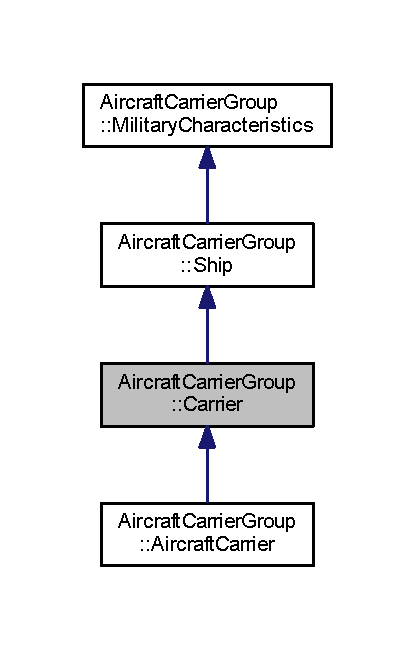
\includegraphics[width=199pt]{class_aircraft_carrier_group_1_1_carrier__inherit__graph}
\end{center}
\end{figure}


Collaboration diagram for Aircraft\+Carrier\+Group\+:\+:Carrier\+:
\nopagebreak
\begin{figure}[H]
\begin{center}
\leavevmode
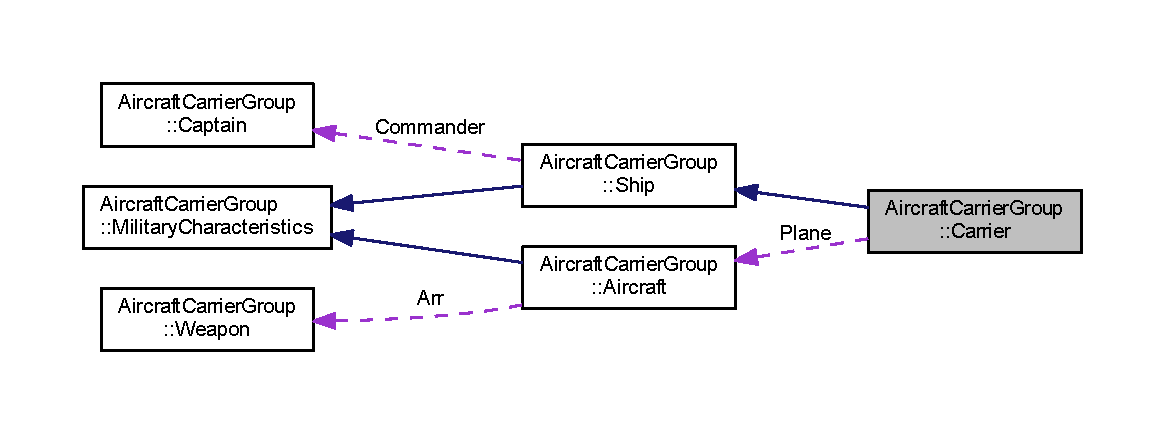
\includegraphics[width=350pt]{class_aircraft_carrier_group_1_1_carrier__coll__graph}
\end{center}
\end{figure}
\subsection*{Public Member Functions}
\begin{DoxyCompactItemize}
\item 
\mbox{\Hypertarget{class_aircraft_carrier_group_1_1_carrier_a6a23c303d5cdf5c336b6cad9ba883340}\label{class_aircraft_carrier_group_1_1_carrier_a6a23c303d5cdf5c336b6cad9ba883340}} 
\mbox{\hyperlink{class_aircraft_carrier_group_1_1_carrier_a6a23c303d5cdf5c336b6cad9ba883340}{Carrier}} ()
\begin{DoxyCompactList}\small\item\em Конструктор по умолчанию \end{DoxyCompactList}\item 
\mbox{\hyperlink{class_aircraft_carrier_group_1_1_carrier_a014facb4517f7f73f860d812099619e1}{Carrier}} (std\+::string Call\+Tmp, const \mbox{\hyperlink{struct_aircraft_carrier_group_1_1_captain}{Captain}} \&Commander\+Tmp, int Crew\+Tmp, const \mbox{\hyperlink{class_aircraft_carrier_group_1_1_military_characteristics}{Military\+Characteristics}} \&Military\+Tmp, int Amount\+P\+Tmp=0, \mbox{\hyperlink{class_aircraft_carrier_group_1_1_aircraft}{Aircraft}} $\ast$Plane\+Tmp=nullptr)
\begin{DoxyCompactList}\small\item\em Инициализирующий конструктор \end{DoxyCompactList}\item 
\mbox{\hyperlink{class_aircraft_carrier_group_1_1_carrier_a9f8e0ddb2e14de4d33cdb85173a5874c}{Carrier}} (const \mbox{\hyperlink{class_aircraft_carrier_group_1_1_carrier}{Carrier}} \&Carrier\+Tmp)
\begin{DoxyCompactList}\small\item\em Копирующий конструктор \end{DoxyCompactList}\item 
\mbox{\Hypertarget{class_aircraft_carrier_group_1_1_carrier_a1bd0a5fd4c5237f0e19aeb93dead2d18}\label{class_aircraft_carrier_group_1_1_carrier_a1bd0a5fd4c5237f0e19aeb93dead2d18}} 
virtual \mbox{\hyperlink{class_aircraft_carrier_group_1_1_carrier_a1bd0a5fd4c5237f0e19aeb93dead2d18}{$\sim$\+Carrier}} ()
\begin{DoxyCompactList}\small\item\em Деструктор \end{DoxyCompactList}\item 
\mbox{\Hypertarget{class_aircraft_carrier_group_1_1_carrier_a1b6a8d9f9d78721cc382c870aa09263a}\label{class_aircraft_carrier_group_1_1_carrier_a1b6a8d9f9d78721cc382c870aa09263a}} 
std\+::ostream \& \mbox{\hyperlink{class_aircraft_carrier_group_1_1_carrier_a1b6a8d9f9d78721cc382c870aa09263a}{print\+Info\+Weapon}} (std\+::ostream \&os) const
\begin{DoxyCompactList}\small\item\em Выводит всю информацию обо всех орудиях на судне \end{DoxyCompactList}\item 
\mbox{\Hypertarget{class_aircraft_carrier_group_1_1_carrier_adfaf335c1a925c8d5c0d441378cc7156}\label{class_aircraft_carrier_group_1_1_carrier_adfaf335c1a925c8d5c0d441378cc7156}} 
int \mbox{\hyperlink{class_aircraft_carrier_group_1_1_carrier_adfaf335c1a925c8d5c0d441378cc7156}{Damage\+All\+Planes}} () const
\begin{DoxyCompactList}\small\item\em Производит расчет разрушений, которые могут нанести все самолеты судна условной цели за единицу времени \end{DoxyCompactList}\item 
virtual int \mbox{\hyperlink{class_aircraft_carrier_group_1_1_carrier_a2829f08d60294321b5d06615d696864e}{Damage\+All\+Weapons}} () const
\begin{DoxyCompactList}\small\item\em Производит расчет разрушений, которые могут нанести все орудия судна условной цели за единицу времени \end{DoxyCompactList}\item 
virtual double \mbox{\hyperlink{class_aircraft_carrier_group_1_1_carrier_aa0e7ab8690d5120c39b5eb1bb58d5709}{Time\+Fire\+All\+Weapons}} () const
\begin{DoxyCompactList}\small\item\em Производит рассчет времени ведения огня всеми орудиями судна с полной скорострельностью \end{DoxyCompactList}\item 
virtual \mbox{\hyperlink{class_aircraft_carrier_group_1_1_carrier}{Carrier}} \& \mbox{\hyperlink{class_aircraft_carrier_group_1_1_carrier_a1ed41e4f12ea2941112fa17adf8eb7a0}{Weapon\+Modification}} (std\+::string Name\+Weapon\+Tmp, const \mbox{\hyperlink{class_aircraft_carrier_group_1_1_weapon}{Weapon}} \&Weapon\+Tmp)
\begin{DoxyCompactList}\small\item\em Функция модифицирует выбранное, из имеющихся на корабле, орудие \end{DoxyCompactList}\item 
virtual \mbox{\hyperlink{class_aircraft_carrier_group_1_1_carrier}{Carrier}} $\ast$ \mbox{\hyperlink{class_aircraft_carrier_group_1_1_carrier_acb567d5ef451d10187f46c34653626e1}{clone}} () const
\begin{DoxyCompactList}\small\item\em Клонирует данный корабль \end{DoxyCompactList}\item 
virtual \mbox{\hyperlink{class_aircraft_carrier_group_1_1_weapon}{Weapon}} $\ast$ \mbox{\hyperlink{class_aircraft_carrier_group_1_1_carrier_a69e4672d2e5b0e7ff0d27e9ec762b828}{get\+Weapon}} (std\+::string Name) const
\begin{DoxyCompactList}\small\item\em Функция получает описатель оружия по его названию \end{DoxyCompactList}\item 
virtual int \mbox{\hyperlink{class_aircraft_carrier_group_1_1_carrier_af6d3cd1b93441f0cdee9c06a8e78bb05}{Amount\+Weapon}} () const
\begin{DoxyCompactList}\small\item\em Возвращает количество вооружения на судне \end{DoxyCompactList}\item 
\mbox{\Hypertarget{class_aircraft_carrier_group_1_1_carrier_adc8ad419feaed9154a980b447e23a159}\label{class_aircraft_carrier_group_1_1_carrier_adc8ad419feaed9154a980b447e23a159}} 
virtual int \mbox{\hyperlink{class_aircraft_carrier_group_1_1_carrier_adc8ad419feaed9154a980b447e23a159}{Type\+Ship}} () const
\begin{DoxyCompactList}\small\item\em Тип данного корабля \end{DoxyCompactList}\item 
\mbox{\Hypertarget{class_aircraft_carrier_group_1_1_carrier_a5140ceccb1365f4e7882c7e2cea7c2a5}\label{class_aircraft_carrier_group_1_1_carrier_a5140ceccb1365f4e7882c7e2cea7c2a5}} 
\mbox{\hyperlink{class_aircraft_carrier_group_1_1_aircraft}{Aircraft}} $\ast$ \mbox{\hyperlink{class_aircraft_carrier_group_1_1_carrier_a5140ceccb1365f4e7882c7e2cea7c2a5}{get\+Air}} (int Number) const
\begin{DoxyCompactList}\small\item\em Возвращет указатель на описатель самолета по его номеру \end{DoxyCompactList}\item 
\mbox{\Hypertarget{class_aircraft_carrier_group_1_1_carrier_abd7c7342ef057fc1d14ec9296631cce8}\label{class_aircraft_carrier_group_1_1_carrier_abd7c7342ef057fc1d14ec9296631cce8}} 
int \mbox{\hyperlink{class_aircraft_carrier_group_1_1_carrier_abd7c7342ef057fc1d14ec9296631cce8}{Amount\+Aircraft}} () const
\begin{DoxyCompactList}\small\item\em Возвращет количество самолетов на палубе \end{DoxyCompactList}\item 
\mbox{\hyperlink{class_aircraft_carrier_group_1_1_carrier}{Carrier}} \& \mbox{\hyperlink{class_aircraft_carrier_group_1_1_carrier_ac85afb17582997d9e5956ff89d22a1e6}{Add\+Aircraft}} (const \mbox{\hyperlink{class_aircraft_carrier_group_1_1_aircraft}{Aircraft}} \&Plane\+Tmp)
\begin{DoxyCompactList}\small\item\em Производит добавление самолета на данный корабль \end{DoxyCompactList}\item 
\mbox{\hyperlink{class_aircraft_carrier_group_1_1_carrier}{Carrier}} \& \mbox{\hyperlink{class_aircraft_carrier_group_1_1_carrier_a23f5d495e4bb570a8abb7ee08cce2d12}{Delete\+Aircraft}} (\mbox{\hyperlink{class_aircraft_carrier_group_1_1_aircraft}{Aircraft}} $\ast$Deleted\+Aircraft=nullptr)
\begin{DoxyCompactList}\small\item\em Производит удаление самолета с корабль  Данная функция производит поиск поиск самолета по его номеру, в случае успеха копирует в буферную переменную (это необходимо для функции переноса самолета с одного корабля на другой), а затем производит его удаление с этого корабля \end{DoxyCompactList}\item 
\mbox{\Hypertarget{class_aircraft_carrier_group_1_1_carrier_a221150a9fd68865af18d06bf14bb052d}\label{class_aircraft_carrier_group_1_1_carrier_a221150a9fd68865af18d06bf14bb052d}} 
double \mbox{\hyperlink{class_aircraft_carrier_group_1_1_carrier_a221150a9fd68865af18d06bf14bb052d}{Max\+Aircraft\+Flyght}} () const
\begin{DoxyCompactList}\small\item\em Производит рассчет времени одновременного полета всех самолетов корабля \end{DoxyCompactList}\item 
\mbox{\Hypertarget{class_aircraft_carrier_group_1_1_carrier_a6f0ad3fe4f9a7e7afc16501bed38dd6b}\label{class_aircraft_carrier_group_1_1_carrier_a6f0ad3fe4f9a7e7afc16501bed38dd6b}} 
double \mbox{\hyperlink{class_aircraft_carrier_group_1_1_carrier_a6f0ad3fe4f9a7e7afc16501bed38dd6b}{Max\+Radius\+Flyght}} () const
\begin{DoxyCompactList}\small\item\em Производит рассчет радиуса действия всех самолетов корабля \end{DoxyCompactList}\item 
std\+::string \mbox{\hyperlink{class_aircraft_carrier_group_1_1_carrier_a5540afe1e3ed0c42d299d3a6dd230585}{Get\+Disguised}} () const
\begin{DoxyCompactList}\small\item\em Функция возвращет названия прикрываемого корабля \end{DoxyCompactList}\end{DoxyCompactItemize}
\subsection*{Protected Member Functions}
\begin{DoxyCompactItemize}
\item 
\mbox{\Hypertarget{class_aircraft_carrier_group_1_1_carrier_a39c9209efcee88accaa52f78f0e27b15}\label{class_aircraft_carrier_group_1_1_carrier_a39c9209efcee88accaa52f78f0e27b15}} 
virtual std\+::ostream \& {\bfseries show} (std\+::ostream \&os) const
\item 
\mbox{\Hypertarget{class_aircraft_carrier_group_1_1_carrier_a46a590f1d91764b992bd3ba38c1f7491}\label{class_aircraft_carrier_group_1_1_carrier_a46a590f1d91764b992bd3ba38c1f7491}} 
virtual std\+::istream \& {\bfseries get} (std\+::istream \&)
\item 
\mbox{\Hypertarget{class_aircraft_carrier_group_1_1_carrier_a33df44dd96c25a3a8d6a6bbf0e3cb5c7}\label{class_aircraft_carrier_group_1_1_carrier_a33df44dd96c25a3a8d6a6bbf0e3cb5c7}} 
virtual std\+::ofstream \& {\bfseries fprint} (std\+::ofstream \&) const
\item 
\mbox{\Hypertarget{class_aircraft_carrier_group_1_1_carrier_a3ba78774821b750009f80b54074f1512}\label{class_aircraft_carrier_group_1_1_carrier_a3ba78774821b750009f80b54074f1512}} 
virtual std\+::ifstream \& {\bfseries fread} (std\+::ifstream \&)
\end{DoxyCompactItemize}
\subsection*{Protected Attributes}
\begin{DoxyCompactItemize}
\item 
\mbox{\Hypertarget{class_aircraft_carrier_group_1_1_carrier_a480a6c273c2bf1b2306bebb827694f79}\label{class_aircraft_carrier_group_1_1_carrier_a480a6c273c2bf1b2306bebb827694f79}} 
int {\bfseries AmountP}
\item 
\mbox{\Hypertarget{class_aircraft_carrier_group_1_1_carrier_ada6d8bb865fbb1c75345c3cf1eb9a55b}\label{class_aircraft_carrier_group_1_1_carrier_ada6d8bb865fbb1c75345c3cf1eb9a55b}} 
\mbox{\hyperlink{class_aircraft_carrier_group_1_1_aircraft}{Aircraft}} $\ast$ {\bfseries Plane}
\end{DoxyCompactItemize}
\subsection*{Friends}
\begin{DoxyCompactItemize}
\item 
\mbox{\Hypertarget{class_aircraft_carrier_group_1_1_carrier_a1256a8df3c81a3c4660dee2cea8b647a}\label{class_aircraft_carrier_group_1_1_carrier_a1256a8df3c81a3c4660dee2cea8b647a}} 
std\+::ostream \& {\bfseries operator$<$$<$} (std\+::ostream \&, const \mbox{\hyperlink{class_aircraft_carrier_group_1_1_carrier}{Carrier}} \&)
\item 
\mbox{\Hypertarget{class_aircraft_carrier_group_1_1_carrier_a6b96a414ec4c3b03dd6994465a4a1b97}\label{class_aircraft_carrier_group_1_1_carrier_a6b96a414ec4c3b03dd6994465a4a1b97}} 
std\+::istream \& {\bfseries operator$>$$>$} (std\+::istream \&, \mbox{\hyperlink{class_aircraft_carrier_group_1_1_carrier}{Carrier}} \&)
\item 
\mbox{\Hypertarget{class_aircraft_carrier_group_1_1_carrier_a6814d89937fdc74abb545c18ec5232e1}\label{class_aircraft_carrier_group_1_1_carrier_a6814d89937fdc74abb545c18ec5232e1}} 
std\+::ofstream \& {\bfseries operator$<$$<$} (std\+::ofstream \&os, const \mbox{\hyperlink{class_aircraft_carrier_group_1_1_carrier}{Carrier}} \&Ship\+Tmp)
\item 
\mbox{\Hypertarget{class_aircraft_carrier_group_1_1_carrier_aa3f27f0e4e7e88bf71fad540abc49871}\label{class_aircraft_carrier_group_1_1_carrier_aa3f27f0e4e7e88bf71fad540abc49871}} 
std\+::ifstream \& {\bfseries operator$>$$>$} (std\+::ifstream \&is, \mbox{\hyperlink{class_aircraft_carrier_group_1_1_carrier}{Carrier}} \&Ship\+Tmp)
\end{DoxyCompactItemize}


\subsection{Detailed Description}
Класс для описания авианосца  Осуществляет хранение всех параметров авиносца и содержит функции, обрабатывающие эти параметры 

\subsection{Constructor \& Destructor Documentation}
\mbox{\Hypertarget{class_aircraft_carrier_group_1_1_carrier_a014facb4517f7f73f860d812099619e1}\label{class_aircraft_carrier_group_1_1_carrier_a014facb4517f7f73f860d812099619e1}} 
\index{Aircraft\+Carrier\+Group\+::\+Carrier@{Aircraft\+Carrier\+Group\+::\+Carrier}!Carrier@{Carrier}}
\index{Carrier@{Carrier}!Aircraft\+Carrier\+Group\+::\+Carrier@{Aircraft\+Carrier\+Group\+::\+Carrier}}
\subsubsection{\texorpdfstring{Carrier()}{Carrier()}\hspace{0.1cm}{\footnotesize\ttfamily [1/2]}}
{\footnotesize\ttfamily Aircraft\+Carrier\+Group\+::\+Carrier\+::\+Carrier (\begin{DoxyParamCaption}\item[{std\+::string}]{Call\+Tmp,  }\item[{const \mbox{\hyperlink{struct_aircraft_carrier_group_1_1_captain}{Captain}} \&}]{Commander\+Tmp,  }\item[{int}]{Crew\+Tmp,  }\item[{const \mbox{\hyperlink{class_aircraft_carrier_group_1_1_military_characteristics}{Military\+Characteristics}} \&}]{Military\+Tmp,  }\item[{int}]{Amount\+P\+Tmp = {\ttfamily 0},  }\item[{\mbox{\hyperlink{class_aircraft_carrier_group_1_1_aircraft}{Aircraft}} $\ast$}]{Plane\+Tmp = {\ttfamily nullptr} }\end{DoxyParamCaption})}



Инициализирующий конструктор 


\begin{DoxyParams}{Parameters}
{\em Call\+Tmp} & Название корабля \\
\hline
{\em Comander\+Tmp} & Капитан судна \\
\hline
{\em Crew\+Tmp} & Количество человек в команде \\
\hline
{\em Military\+Tmp} & Хранит общие характеристики техники \\
\hline
{\em Amount\+P\+Tmp} & Количество самолетов на палубе корабля \\
\hline
{\em Plane\+Tmp} & Содержит описатели каждого из самолетов \\
\hline
\end{DoxyParams}
\mbox{\Hypertarget{class_aircraft_carrier_group_1_1_carrier_a9f8e0ddb2e14de4d33cdb85173a5874c}\label{class_aircraft_carrier_group_1_1_carrier_a9f8e0ddb2e14de4d33cdb85173a5874c}} 
\index{Aircraft\+Carrier\+Group\+::\+Carrier@{Aircraft\+Carrier\+Group\+::\+Carrier}!Carrier@{Carrier}}
\index{Carrier@{Carrier}!Aircraft\+Carrier\+Group\+::\+Carrier@{Aircraft\+Carrier\+Group\+::\+Carrier}}
\subsubsection{\texorpdfstring{Carrier()}{Carrier()}\hspace{0.1cm}{\footnotesize\ttfamily [2/2]}}
{\footnotesize\ttfamily Aircraft\+Carrier\+Group\+::\+Carrier\+::\+Carrier (\begin{DoxyParamCaption}\item[{const \mbox{\hyperlink{class_aircraft_carrier_group_1_1_carrier}{Carrier}} \&}]{Carrier\+Tmp }\end{DoxyParamCaption})}



Копирующий конструктор 


\begin{DoxyParams}{Parameters}
{\em Carrier\+Tmp} & Описатель авианосца \\
\hline
\end{DoxyParams}


\subsection{Member Function Documentation}
\mbox{\Hypertarget{class_aircraft_carrier_group_1_1_carrier_ac85afb17582997d9e5956ff89d22a1e6}\label{class_aircraft_carrier_group_1_1_carrier_ac85afb17582997d9e5956ff89d22a1e6}} 
\index{Aircraft\+Carrier\+Group\+::\+Carrier@{Aircraft\+Carrier\+Group\+::\+Carrier}!Add\+Aircraft@{Add\+Aircraft}}
\index{Add\+Aircraft@{Add\+Aircraft}!Aircraft\+Carrier\+Group\+::\+Carrier@{Aircraft\+Carrier\+Group\+::\+Carrier}}
\subsubsection{\texorpdfstring{Add\+Aircraft()}{AddAircraft()}}
{\footnotesize\ttfamily \mbox{\hyperlink{class_aircraft_carrier_group_1_1_carrier}{Carrier}} \& Aircraft\+Carrier\+Group\+::\+Carrier\+::\+Add\+Aircraft (\begin{DoxyParamCaption}\item[{const \mbox{\hyperlink{class_aircraft_carrier_group_1_1_aircraft}{Aircraft}} \&}]{Plane\+Tmp }\end{DoxyParamCaption})}



Производит добавление самолета на данный корабль 


\begin{DoxyParams}{Parameters}
{\em Plane\+Tmp} & Описатель самолета \\
\hline
\end{DoxyParams}
\mbox{\Hypertarget{class_aircraft_carrier_group_1_1_carrier_af6d3cd1b93441f0cdee9c06a8e78bb05}\label{class_aircraft_carrier_group_1_1_carrier_af6d3cd1b93441f0cdee9c06a8e78bb05}} 
\index{Aircraft\+Carrier\+Group\+::\+Carrier@{Aircraft\+Carrier\+Group\+::\+Carrier}!Amount\+Weapon@{Amount\+Weapon}}
\index{Amount\+Weapon@{Amount\+Weapon}!Aircraft\+Carrier\+Group\+::\+Carrier@{Aircraft\+Carrier\+Group\+::\+Carrier}}
\subsubsection{\texorpdfstring{Amount\+Weapon()}{AmountWeapon()}}
{\footnotesize\ttfamily virtual int Aircraft\+Carrier\+Group\+::\+Carrier\+::\+Amount\+Weapon (\begin{DoxyParamCaption}{ }\end{DoxyParamCaption}) const\hspace{0.3cm}{\ttfamily [inline]}, {\ttfamily [virtual]}}



Возвращает количество вооружения на судне 


\begin{DoxyExceptions}{Exceptions}
{\em Invalid\+Operation} & При попытке получить количество орудий на корабле, поскольку этот тип кораблей не может иметь вооружения на борту \\
\hline
\end{DoxyExceptions}


Implements \mbox{\hyperlink{class_aircraft_carrier_group_1_1_ship_ab082a4331c038ece44b7304b7d3c212c}{Aircraft\+Carrier\+Group\+::\+Ship}}.



Reimplemented in \mbox{\hyperlink{class_aircraft_carrier_group_1_1_aircraft_carrier_abddfdb193451143aa371c5fb86705afb}{Aircraft\+Carrier\+Group\+::\+Aircraft\+Carrier}}.

\mbox{\Hypertarget{class_aircraft_carrier_group_1_1_carrier_acb567d5ef451d10187f46c34653626e1}\label{class_aircraft_carrier_group_1_1_carrier_acb567d5ef451d10187f46c34653626e1}} 
\index{Aircraft\+Carrier\+Group\+::\+Carrier@{Aircraft\+Carrier\+Group\+::\+Carrier}!clone@{clone}}
\index{clone@{clone}!Aircraft\+Carrier\+Group\+::\+Carrier@{Aircraft\+Carrier\+Group\+::\+Carrier}}
\subsubsection{\texorpdfstring{clone()}{clone()}}
{\footnotesize\ttfamily virtual \mbox{\hyperlink{class_aircraft_carrier_group_1_1_carrier}{Carrier}}$\ast$ Aircraft\+Carrier\+Group\+::\+Carrier\+::clone (\begin{DoxyParamCaption}{ }\end{DoxyParamCaption}) const\hspace{0.3cm}{\ttfamily [inline]}, {\ttfamily [virtual]}}



Клонирует данный корабль 

\begin{DoxyReturn}{Returns}
Возвращает указатель на область памяти, в котором хранится копия этого корабля 
\end{DoxyReturn}


Implements \mbox{\hyperlink{class_aircraft_carrier_group_1_1_ship_aec409c849026fa7d242fdd7de7ae9f02}{Aircraft\+Carrier\+Group\+::\+Ship}}.



Reimplemented in \mbox{\hyperlink{class_aircraft_carrier_group_1_1_aircraft_carrier_ab2f921c586a31f9933874f437baf9c16}{Aircraft\+Carrier\+Group\+::\+Aircraft\+Carrier}}.

Here is the call graph for this function\+:
\nopagebreak
\begin{figure}[H]
\begin{center}
\leavevmode
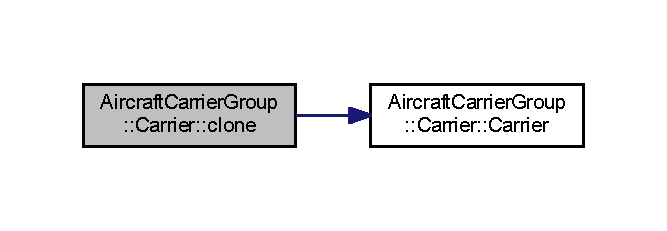
\includegraphics[width=320pt]{class_aircraft_carrier_group_1_1_carrier_acb567d5ef451d10187f46c34653626e1_cgraph}
\end{center}
\end{figure}
\mbox{\Hypertarget{class_aircraft_carrier_group_1_1_carrier_a2829f08d60294321b5d06615d696864e}\label{class_aircraft_carrier_group_1_1_carrier_a2829f08d60294321b5d06615d696864e}} 
\index{Aircraft\+Carrier\+Group\+::\+Carrier@{Aircraft\+Carrier\+Group\+::\+Carrier}!Damage\+All\+Weapons@{Damage\+All\+Weapons}}
\index{Damage\+All\+Weapons@{Damage\+All\+Weapons}!Aircraft\+Carrier\+Group\+::\+Carrier@{Aircraft\+Carrier\+Group\+::\+Carrier}}
\subsubsection{\texorpdfstring{Damage\+All\+Weapons()}{DamageAllWeapons()}}
{\footnotesize\ttfamily virtual int Aircraft\+Carrier\+Group\+::\+Carrier\+::\+Damage\+All\+Weapons (\begin{DoxyParamCaption}{ }\end{DoxyParamCaption}) const\hspace{0.3cm}{\ttfamily [inline]}, {\ttfamily [virtual]}}



Производит расчет разрушений, которые могут нанести все орудия судна условной цели за единицу времени 


\begin{DoxyExceptions}{Exceptions}
{\em Invalid\+Operation} & При попытке рассчета урона, наносимого всеми орудиями судна, поскольку этот тип кораблей не может иметь вооружения на борту \\
\hline
\end{DoxyExceptions}


Implements \mbox{\hyperlink{class_aircraft_carrier_group_1_1_ship_a025ad4bfa82e6ff5539d53ab899bd37f}{Aircraft\+Carrier\+Group\+::\+Ship}}.



Reimplemented in \mbox{\hyperlink{class_aircraft_carrier_group_1_1_aircraft_carrier_ab2caba5f25f136dff2354539b47ff68c}{Aircraft\+Carrier\+Group\+::\+Aircraft\+Carrier}}.

\mbox{\Hypertarget{class_aircraft_carrier_group_1_1_carrier_a23f5d495e4bb570a8abb7ee08cce2d12}\label{class_aircraft_carrier_group_1_1_carrier_a23f5d495e4bb570a8abb7ee08cce2d12}} 
\index{Aircraft\+Carrier\+Group\+::\+Carrier@{Aircraft\+Carrier\+Group\+::\+Carrier}!Delete\+Aircraft@{Delete\+Aircraft}}
\index{Delete\+Aircraft@{Delete\+Aircraft}!Aircraft\+Carrier\+Group\+::\+Carrier@{Aircraft\+Carrier\+Group\+::\+Carrier}}
\subsubsection{\texorpdfstring{Delete\+Aircraft()}{DeleteAircraft()}}
{\footnotesize\ttfamily \mbox{\hyperlink{class_aircraft_carrier_group_1_1_carrier}{Carrier}} \& Aircraft\+Carrier\+Group\+::\+Carrier\+::\+Delete\+Aircraft (\begin{DoxyParamCaption}\item[{\mbox{\hyperlink{class_aircraft_carrier_group_1_1_aircraft}{Aircraft}} $\ast$}]{Deleted\+Aircraft = {\ttfamily nullptr} }\end{DoxyParamCaption})}



Производит удаление самолета с корабль  Данная функция производит поиск поиск самолета по его номеру, в случае успеха копирует в буферную переменную (это необходимо для функции переноса самолета с одного корабля на другой), а затем производит его удаление с этого корабля 


\begin{DoxyParams}[1]{Parameters}
\mbox{\tt out}  & {\em Deleted\+Aircraft} & Копия удаленного самолета \\
\hline
\end{DoxyParams}
\mbox{\Hypertarget{class_aircraft_carrier_group_1_1_carrier_a5540afe1e3ed0c42d299d3a6dd230585}\label{class_aircraft_carrier_group_1_1_carrier_a5540afe1e3ed0c42d299d3a6dd230585}} 
\index{Aircraft\+Carrier\+Group\+::\+Carrier@{Aircraft\+Carrier\+Group\+::\+Carrier}!Get\+Disguised@{Get\+Disguised}}
\index{Get\+Disguised@{Get\+Disguised}!Aircraft\+Carrier\+Group\+::\+Carrier@{Aircraft\+Carrier\+Group\+::\+Carrier}}
\subsubsection{\texorpdfstring{Get\+Disguised()}{GetDisguised()}}
{\footnotesize\ttfamily std\+::string Aircraft\+Carrier\+Group\+::\+Carrier\+::\+Get\+Disguised (\begin{DoxyParamCaption}{ }\end{DoxyParamCaption}) const\hspace{0.3cm}{\ttfamily [inline]}, {\ttfamily [virtual]}}



Функция возвращет названия прикрываемого корабля 


\begin{DoxyExceptions}{Exceptions}
{\em Invalid\+Ship\+Type} & При попытке получить названия прикрываемого корабля, поскольку этот тип кораблей не может иметь прикрываемого корабля \\
\hline
\end{DoxyExceptions}


Implements \mbox{\hyperlink{class_aircraft_carrier_group_1_1_ship_a6455eb63c95dd3598b45b92e42e7f84d}{Aircraft\+Carrier\+Group\+::\+Ship}}.

\mbox{\Hypertarget{class_aircraft_carrier_group_1_1_carrier_a69e4672d2e5b0e7ff0d27e9ec762b828}\label{class_aircraft_carrier_group_1_1_carrier_a69e4672d2e5b0e7ff0d27e9ec762b828}} 
\index{Aircraft\+Carrier\+Group\+::\+Carrier@{Aircraft\+Carrier\+Group\+::\+Carrier}!get\+Weapon@{get\+Weapon}}
\index{get\+Weapon@{get\+Weapon}!Aircraft\+Carrier\+Group\+::\+Carrier@{Aircraft\+Carrier\+Group\+::\+Carrier}}
\subsubsection{\texorpdfstring{get\+Weapon()}{getWeapon()}}
{\footnotesize\ttfamily virtual \mbox{\hyperlink{class_aircraft_carrier_group_1_1_weapon}{Weapon}}$\ast$ Aircraft\+Carrier\+Group\+::\+Carrier\+::get\+Weapon (\begin{DoxyParamCaption}\item[{std\+::string}]{Name }\end{DoxyParamCaption}) const\hspace{0.3cm}{\ttfamily [inline]}, {\ttfamily [virtual]}}



Функция получает описатель оружия по его названию 


\begin{DoxyParams}{Parameters}
{\em Name} & Название оружия \\
\hline
\end{DoxyParams}
\begin{DoxyReturn}{Returns}
Возвращает указатель на область памяти, в котором хранится описатель найденного оружия 
\end{DoxyReturn}

\begin{DoxyExceptions}{Exceptions}
{\em Invalid\+Operation} & При попытке получить описатель орудия корабля по его названию, поскольку этот тип кораблей не может иметь вооружения на борту \\
\hline
\end{DoxyExceptions}


Implements \mbox{\hyperlink{class_aircraft_carrier_group_1_1_ship_a8ac6e8e9ed4f997a5f02fda7e049cd6d}{Aircraft\+Carrier\+Group\+::\+Ship}}.



Reimplemented in \mbox{\hyperlink{class_aircraft_carrier_group_1_1_aircraft_carrier_aa7839178084e4f749592e02d2d8e93a4}{Aircraft\+Carrier\+Group\+::\+Aircraft\+Carrier}}.

\mbox{\Hypertarget{class_aircraft_carrier_group_1_1_carrier_aa0e7ab8690d5120c39b5eb1bb58d5709}\label{class_aircraft_carrier_group_1_1_carrier_aa0e7ab8690d5120c39b5eb1bb58d5709}} 
\index{Aircraft\+Carrier\+Group\+::\+Carrier@{Aircraft\+Carrier\+Group\+::\+Carrier}!Time\+Fire\+All\+Weapons@{Time\+Fire\+All\+Weapons}}
\index{Time\+Fire\+All\+Weapons@{Time\+Fire\+All\+Weapons}!Aircraft\+Carrier\+Group\+::\+Carrier@{Aircraft\+Carrier\+Group\+::\+Carrier}}
\subsubsection{\texorpdfstring{Time\+Fire\+All\+Weapons()}{TimeFireAllWeapons()}}
{\footnotesize\ttfamily virtual double Aircraft\+Carrier\+Group\+::\+Carrier\+::\+Time\+Fire\+All\+Weapons (\begin{DoxyParamCaption}{ }\end{DoxyParamCaption}) const\hspace{0.3cm}{\ttfamily [inline]}, {\ttfamily [virtual]}}



Производит рассчет времени ведения огня всеми орудиями судна с полной скорострельностью 


\begin{DoxyExceptions}{Exceptions}
{\em Invalid\+Operation} & При попытке рассчета врмени ведения всеми орудиями судна, поскольку этот тип кораблей не может иметь вооружения на борту \\
\hline
\end{DoxyExceptions}


Implements \mbox{\hyperlink{class_aircraft_carrier_group_1_1_ship_a255221ad52eec6bd027854b1fdb18187}{Aircraft\+Carrier\+Group\+::\+Ship}}.



Reimplemented in \mbox{\hyperlink{class_aircraft_carrier_group_1_1_aircraft_carrier_a6613d24d38f7a28d20f35437bc069f98}{Aircraft\+Carrier\+Group\+::\+Aircraft\+Carrier}}.

\mbox{\Hypertarget{class_aircraft_carrier_group_1_1_carrier_a1ed41e4f12ea2941112fa17adf8eb7a0}\label{class_aircraft_carrier_group_1_1_carrier_a1ed41e4f12ea2941112fa17adf8eb7a0}} 
\index{Aircraft\+Carrier\+Group\+::\+Carrier@{Aircraft\+Carrier\+Group\+::\+Carrier}!Weapon\+Modification@{Weapon\+Modification}}
\index{Weapon\+Modification@{Weapon\+Modification}!Aircraft\+Carrier\+Group\+::\+Carrier@{Aircraft\+Carrier\+Group\+::\+Carrier}}
\subsubsection{\texorpdfstring{Weapon\+Modification()}{WeaponModification()}}
{\footnotesize\ttfamily virtual \mbox{\hyperlink{class_aircraft_carrier_group_1_1_carrier}{Carrier}}\& Aircraft\+Carrier\+Group\+::\+Carrier\+::\+Weapon\+Modification (\begin{DoxyParamCaption}\item[{std\+::string}]{Name\+Weapon\+Tmp,  }\item[{const \mbox{\hyperlink{class_aircraft_carrier_group_1_1_weapon}{Weapon}} \&}]{Weapon\+Tmp }\end{DoxyParamCaption})\hspace{0.3cm}{\ttfamily [inline]}, {\ttfamily [virtual]}}



Функция модифицирует выбранное, из имеющихся на корабле, орудие 


\begin{DoxyParams}{Parameters}
{\em Name\+Weapon\+Tmp} & Названия орудия, которое надо модифицировать \\
\hline
{\em Weapon\+Tmp} & Новое орудие \\
\hline
\end{DoxyParams}

\begin{DoxyExceptions}{Exceptions}
{\em Invalid\+Operation} & При попытке модификации орудия судна, поскольку этот тип кораблей не может иметь вооружения на борту \\
\hline
\end{DoxyExceptions}


Implements \mbox{\hyperlink{class_aircraft_carrier_group_1_1_ship_a3f91c1ad2960c095cfd88e85df0a3990}{Aircraft\+Carrier\+Group\+::\+Ship}}.



The documentation for this class was generated from the following files\+:\begin{DoxyCompactItemize}
\item 
C\+:/\+Users/\+Sema/\+Desktop/\+Code\+Forces/\+Labs/4th\+\_\+\+Lab + library connection/\+Library/\mbox{\hyperlink{_carrier_8h}{Carrier.\+h}}\item 
C\+:/\+Users/\+Sema/\+Desktop/\+Code\+Forces/\+Labs/4th\+\_\+\+Lab + library connection/\+Library/Carrier.\+cpp\end{DoxyCompactItemize}

\hypertarget{class_aircraft_carrier_group_1_1_const_fleet_it}{}\section{Aircraft\+Carrier\+Group\+:\+:Const\+Fleet\+It Class Reference}
\label{class_aircraft_carrier_group_1_1_const_fleet_it}\index{Aircraft\+Carrier\+Group\+::\+Const\+Fleet\+It@{Aircraft\+Carrier\+Group\+::\+Const\+Fleet\+It}}


Класс-\/итератор для класса \mbox{\hyperlink{class_aircraft_carrier_group_1_1_fleet}{Fleet}}  При его помощи осуществляется доступ к элементам контейнера класса \mbox{\hyperlink{class_aircraft_carrier_group_1_1_fleet}{Fleet}}.  




{\ttfamily \#include $<$Fleet.\+h$>$}

\subsection*{Public Member Functions}
\begin{DoxyCompactItemize}
\item 
\mbox{\Hypertarget{class_aircraft_carrier_group_1_1_const_fleet_it_a4813f5fe58d256d4dccc8ba7c1425b5c}\label{class_aircraft_carrier_group_1_1_const_fleet_it_a4813f5fe58d256d4dccc8ba7c1425b5c}} 
\mbox{\hyperlink{class_aircraft_carrier_group_1_1_const_fleet_it_a4813f5fe58d256d4dccc8ba7c1425b5c}{Const\+Fleet\+It}} ()
\begin{DoxyCompactList}\small\item\em Конструктор по умолчанию \end{DoxyCompactList}\item 
\mbox{\hyperlink{class_aircraft_carrier_group_1_1_const_fleet_it_a7e7d3013d5dada354b4b39b5566d096f}{Const\+Fleet\+It}} (\mbox{\hyperlink{class__map}{\+\_\+map}}$<$ std\+::string, \mbox{\hyperlink{class_aircraft_carrier_group_1_1_ship}{Ship}} $\ast$$>$\+::\+\_\+map\+\_\+const\+\_\+it it)
\begin{DoxyCompactList}\small\item\em Инициализирующий конструктор \end{DoxyCompactList}\item 
\mbox{\Hypertarget{class_aircraft_carrier_group_1_1_const_fleet_it_a83aac6a7725d7ead768706048f89f0e3}\label{class_aircraft_carrier_group_1_1_const_fleet_it_a83aac6a7725d7ead768706048f89f0e3}} 
int {\bfseries operator!=} (const \mbox{\hyperlink{class_aircraft_carrier_group_1_1_const_fleet_it}{Const\+Fleet\+It}} \&) const
\item 
\mbox{\Hypertarget{class_aircraft_carrier_group_1_1_const_fleet_it_ac050e45aa19318a687db19798d4ec555}\label{class_aircraft_carrier_group_1_1_const_fleet_it_ac050e45aa19318a687db19798d4ec555}} 
int {\bfseries operator==} (const \mbox{\hyperlink{class_aircraft_carrier_group_1_1_const_fleet_it}{Const\+Fleet\+It}} \&) const
\item 
\mbox{\Hypertarget{class_aircraft_carrier_group_1_1_const_fleet_it_addc1d662e39282c0ffc730c5121b699b}\label{class_aircraft_carrier_group_1_1_const_fleet_it_addc1d662e39282c0ffc730c5121b699b}} 
const \mbox{\hyperlink{struct__pair}{\+\_\+pair}}$<$ std\+::string, \mbox{\hyperlink{class_aircraft_carrier_group_1_1_ship}{Ship}} $\ast$ $>$ \& {\bfseries operator$\ast$} ()
\item 
\mbox{\Hypertarget{class_aircraft_carrier_group_1_1_const_fleet_it_afddb11222693e0b902a92368ff15c9db}\label{class_aircraft_carrier_group_1_1_const_fleet_it_afddb11222693e0b902a92368ff15c9db}} 
const \mbox{\hyperlink{struct__pair}{\+\_\+pair}}$<$ std\+::string, \mbox{\hyperlink{class_aircraft_carrier_group_1_1_ship}{Ship}} $\ast$ $>$ $\ast$ {\bfseries operator-\/$>$} ()
\item 
\mbox{\Hypertarget{class_aircraft_carrier_group_1_1_const_fleet_it_a6093690222af9b7f8d154bb54710a312}\label{class_aircraft_carrier_group_1_1_const_fleet_it_a6093690222af9b7f8d154bb54710a312}} 
\mbox{\hyperlink{class_aircraft_carrier_group_1_1_const_fleet_it}{Const\+Fleet\+It}} \& {\bfseries operator++} ()
\item 
\mbox{\Hypertarget{class_aircraft_carrier_group_1_1_const_fleet_it_ac63410fcbead3116bf166251236d4d05}\label{class_aircraft_carrier_group_1_1_const_fleet_it_ac63410fcbead3116bf166251236d4d05}} 
\mbox{\hyperlink{class_aircraft_carrier_group_1_1_const_fleet_it}{Const\+Fleet\+It}} {\bfseries operator++} (int)
\end{DoxyCompactItemize}


\subsection{Detailed Description}
Класс-\/итератор для класса \mbox{\hyperlink{class_aircraft_carrier_group_1_1_fleet}{Fleet}}  При его помощи осуществляется доступ к элементам контейнера класса \mbox{\hyperlink{class_aircraft_carrier_group_1_1_fleet}{Fleet}}. 

\subsection{Constructor \& Destructor Documentation}
\mbox{\Hypertarget{class_aircraft_carrier_group_1_1_const_fleet_it_a7e7d3013d5dada354b4b39b5566d096f}\label{class_aircraft_carrier_group_1_1_const_fleet_it_a7e7d3013d5dada354b4b39b5566d096f}} 
\index{Aircraft\+Carrier\+Group\+::\+Const\+Fleet\+It@{Aircraft\+Carrier\+Group\+::\+Const\+Fleet\+It}!Const\+Fleet\+It@{Const\+Fleet\+It}}
\index{Const\+Fleet\+It@{Const\+Fleet\+It}!Aircraft\+Carrier\+Group\+::\+Const\+Fleet\+It@{Aircraft\+Carrier\+Group\+::\+Const\+Fleet\+It}}
\subsubsection{\texorpdfstring{Const\+Fleet\+It()}{ConstFleetIt()}}
{\footnotesize\ttfamily Aircraft\+Carrier\+Group\+::\+Const\+Fleet\+It\+::\+Const\+Fleet\+It (\begin{DoxyParamCaption}\item[{\mbox{\hyperlink{class__map}{\+\_\+map}}$<$ std\+::string, \mbox{\hyperlink{class_aircraft_carrier_group_1_1_ship}{Ship}} $\ast$$>$\+::\+\_\+map\+\_\+const\+\_\+it}]{it }\end{DoxyParamCaption})\hspace{0.3cm}{\ttfamily [inline]}}



Инициализирующий конструктор 


\begin{DoxyParams}{Parameters}
{\em it} & Константный итератор класса \mbox{\hyperlink{class_aircraft_carrier_group_1_1_fleet}{Fleet}} \\
\hline
\end{DoxyParams}


The documentation for this class was generated from the following files\+:\begin{DoxyCompactItemize}
\item 
C\+:/\+Users/\+Sema/\+Desktop/\+Code\+Forces/\+Labs/4th\+\_\+\+Lab + library connection/\+Library/\mbox{\hyperlink{_fleet_8h}{Fleet.\+h}}\item 
C\+:/\+Users/\+Sema/\+Desktop/\+Code\+Forces/\+Labs/4th\+\_\+\+Lab + library connection/\+Library/Fleet.\+cpp\end{DoxyCompactItemize}

\hypertarget{class_aircraft_carrier_group_1_1_cover_ship}{}\section{Aircraft\+Carrier\+Group\+:\+:Cover\+Ship Class Reference}
\label{class_aircraft_carrier_group_1_1_cover_ship}\index{Aircraft\+Carrier\+Group\+::\+Cover\+Ship@{Aircraft\+Carrier\+Group\+::\+Cover\+Ship}}


Класс для описания судна прикрытия  Осуществляет хранение всех параметров судна прикрытия и содержит функции, обрабатывающие эти параметры  




{\ttfamily \#include $<$Cover\+Ship.\+h$>$}



Inheritance diagram for Aircraft\+Carrier\+Group\+:\+:Cover\+Ship\+:
\nopagebreak
\begin{figure}[H]
\begin{center}
\leavevmode
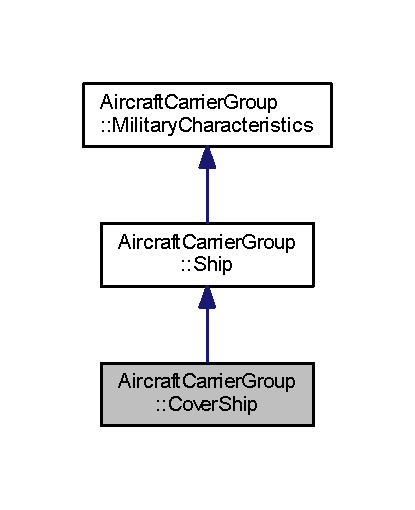
\includegraphics[width=199pt]{class_aircraft_carrier_group_1_1_cover_ship__inherit__graph}
\end{center}
\end{figure}


Collaboration diagram for Aircraft\+Carrier\+Group\+:\+:Cover\+Ship\+:
\nopagebreak
\begin{figure}[H]
\begin{center}
\leavevmode
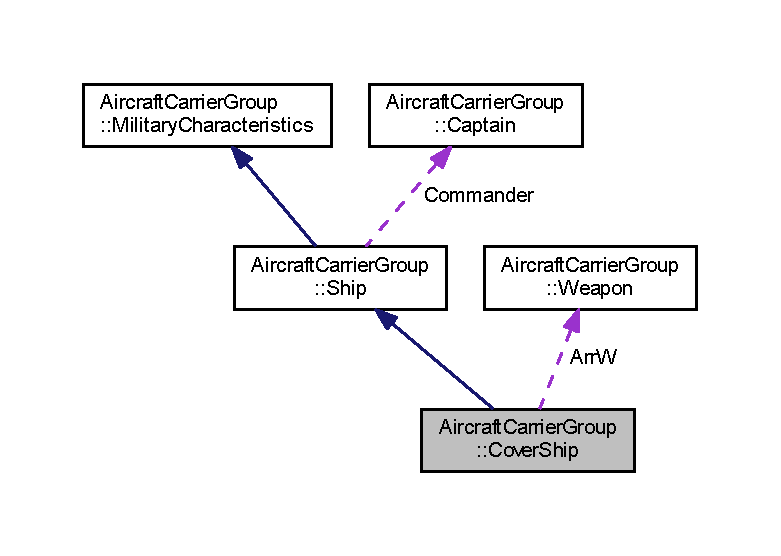
\includegraphics[width=350pt]{class_aircraft_carrier_group_1_1_cover_ship__coll__graph}
\end{center}
\end{figure}
\subsection*{Public Member Functions}
\begin{DoxyCompactItemize}
\item 
\mbox{\Hypertarget{class_aircraft_carrier_group_1_1_cover_ship_aa6c11517d19279d5a7387a1efc2f7a0f}\label{class_aircraft_carrier_group_1_1_cover_ship_aa6c11517d19279d5a7387a1efc2f7a0f}} 
\mbox{\hyperlink{class_aircraft_carrier_group_1_1_cover_ship_aa6c11517d19279d5a7387a1efc2f7a0f}{Cover\+Ship}} ()
\begin{DoxyCompactList}\small\item\em Конструктор по умолчанию \end{DoxyCompactList}\item 
\mbox{\hyperlink{class_aircraft_carrier_group_1_1_cover_ship_a3735bd14678da33bd128266774d21f64}{Cover\+Ship}} (std\+::string Call\+Tmp, const \mbox{\hyperlink{struct_aircraft_carrier_group_1_1_captain}{Captain}} \&Commander\+Tmp, int Crew\+Tmp, const \mbox{\hyperlink{class_aircraft_carrier_group_1_1_military_characteristics}{Military\+Characteristics}} \&Military\+Tmp, std\+::string Disguised\+Tmp, int Amount\+Tmp, \mbox{\hyperlink{class_aircraft_carrier_group_1_1_weapon}{Weapon}} $\ast$Arr\+Tmp)
\begin{DoxyCompactList}\small\item\em Инициализирующий конструктор \end{DoxyCompactList}\item 
\mbox{\hyperlink{class_aircraft_carrier_group_1_1_cover_ship_a2d57e8dba8f2e9abc30dececa2d7cfe2}{Cover\+Ship}} (const \mbox{\hyperlink{class_aircraft_carrier_group_1_1_cover_ship}{Cover\+Ship}} \&Cover\+Ship\+Tmp)
\begin{DoxyCompactList}\small\item\em Копирующий конструктор \end{DoxyCompactList}\item 
\mbox{\Hypertarget{class_aircraft_carrier_group_1_1_cover_ship_a495afaecdaac83ce1358abbded27e226}\label{class_aircraft_carrier_group_1_1_cover_ship_a495afaecdaac83ce1358abbded27e226}} 
\mbox{\hyperlink{class_aircraft_carrier_group_1_1_cover_ship_a495afaecdaac83ce1358abbded27e226}{$\sim$\+Cover\+Ship}} ()
\begin{DoxyCompactList}\small\item\em Деструктор \end{DoxyCompactList}\item 
\mbox{\Hypertarget{class_aircraft_carrier_group_1_1_cover_ship_ae77dfb4b38d2d338c6189d10f1a56dc9}\label{class_aircraft_carrier_group_1_1_cover_ship_ae77dfb4b38d2d338c6189d10f1a56dc9}} 
std\+::ostream \& \mbox{\hyperlink{class_aircraft_carrier_group_1_1_cover_ship_ae77dfb4b38d2d338c6189d10f1a56dc9}{print\+Info\+Weapon}} (std\+::ostream \&os) const
\begin{DoxyCompactList}\small\item\em Выводит всю информацию обо всех орудиях на судне \end{DoxyCompactList}\item 
\mbox{\hyperlink{class_aircraft_carrier_group_1_1_cover_ship}{Cover\+Ship}} \& \mbox{\hyperlink{class_aircraft_carrier_group_1_1_cover_ship_a135b4e20acbdb6bfbcb2cbb6df855d09}{Weapon\+Modification}} (std\+::string Name\+Weapon\+Tmp, const \mbox{\hyperlink{class_aircraft_carrier_group_1_1_weapon}{Weapon}} \&Weapon\+Tmp)
\begin{DoxyCompactList}\small\item\em Функция модифицирует выбранное, из имеющихся на корабле, орудие \end{DoxyCompactList}\item 
\mbox{\Hypertarget{class_aircraft_carrier_group_1_1_cover_ship_abb7d3a8b6537811c8daf0574f6b7af59}\label{class_aircraft_carrier_group_1_1_cover_ship_abb7d3a8b6537811c8daf0574f6b7af59}} 
double \mbox{\hyperlink{class_aircraft_carrier_group_1_1_cover_ship_abb7d3a8b6537811c8daf0574f6b7af59}{Time\+Fire\+All\+Weapons}} () const
\begin{DoxyCompactList}\small\item\em Производит рассчет времени ведения огня всеми орудиями судна с полной скорострельностью \end{DoxyCompactList}\item 
int \mbox{\hyperlink{class_aircraft_carrier_group_1_1_cover_ship_a3a08ec471959146e36e3d6c2fccf2159}{Damage\+All\+Planes}} () const
\begin{DoxyCompactList}\small\item\em Производит расчет разрушений, которые могут нанести все самолеты судна условной цели за единицу времени \end{DoxyCompactList}\item 
\mbox{\Hypertarget{class_aircraft_carrier_group_1_1_cover_ship_a2e880c60db67934fba685100eec7ec84}\label{class_aircraft_carrier_group_1_1_cover_ship_a2e880c60db67934fba685100eec7ec84}} 
int \mbox{\hyperlink{class_aircraft_carrier_group_1_1_cover_ship_a2e880c60db67934fba685100eec7ec84}{Damage\+All\+Weapons}} () const
\begin{DoxyCompactList}\small\item\em Производит расчет разрушений, которые могут нанести все орудия судна условной цели за единицу времени \end{DoxyCompactList}\item 
\mbox{\hyperlink{class_aircraft_carrier_group_1_1_cover_ship}{Cover\+Ship}} $\ast$ \mbox{\hyperlink{class_aircraft_carrier_group_1_1_cover_ship_aa6a5b007f5e05f9ad5cc300b8958309a}{clone}} () const
\begin{DoxyCompactList}\small\item\em Клонирует данный корабль \end{DoxyCompactList}\item 
\mbox{\hyperlink{class_aircraft_carrier_group_1_1_weapon}{Weapon}} $\ast$ \mbox{\hyperlink{class_aircraft_carrier_group_1_1_cover_ship_ab587c598ab12561d4ecad32c5f55a04e}{get\+Weapon}} (std\+::string Name) const
\begin{DoxyCompactList}\small\item\em Функция получает описатель оружия по его названию \end{DoxyCompactList}\item 
\mbox{\Hypertarget{class_aircraft_carrier_group_1_1_cover_ship_a256c7ec80309594f70f3c2e91b9b59d7}\label{class_aircraft_carrier_group_1_1_cover_ship_a256c7ec80309594f70f3c2e91b9b59d7}} 
int \mbox{\hyperlink{class_aircraft_carrier_group_1_1_cover_ship_a256c7ec80309594f70f3c2e91b9b59d7}{Amount\+Weapon}} () const
\begin{DoxyCompactList}\small\item\em Возвращает количество вооружения на судне \end{DoxyCompactList}\item 
\mbox{\Hypertarget{class_aircraft_carrier_group_1_1_cover_ship_a0cc75b445352e2c2c816d9a31884372b}\label{class_aircraft_carrier_group_1_1_cover_ship_a0cc75b445352e2c2c816d9a31884372b}} 
int \mbox{\hyperlink{class_aircraft_carrier_group_1_1_cover_ship_a0cc75b445352e2c2c816d9a31884372b}{Type\+Ship}} () const
\begin{DoxyCompactList}\small\item\em Тип данного корабля \end{DoxyCompactList}\item 
int \mbox{\hyperlink{class_aircraft_carrier_group_1_1_cover_ship_ac53b388322ccc63153ffc6edd2811d7c}{Amount\+Aircraft}} () const
\begin{DoxyCompactList}\small\item\em Возвращет количество самолетов на палубе \end{DoxyCompactList}\item 
\mbox{\Hypertarget{class_aircraft_carrier_group_1_1_cover_ship_a9886f32975ab712d4ea697de7cfbbed9}\label{class_aircraft_carrier_group_1_1_cover_ship_a9886f32975ab712d4ea697de7cfbbed9}} 
std\+::string \mbox{\hyperlink{class_aircraft_carrier_group_1_1_cover_ship_a9886f32975ab712d4ea697de7cfbbed9}{Get\+Disguised}} () const
\begin{DoxyCompactList}\small\item\em Возвращет название прикрываемого корабля \end{DoxyCompactList}\end{DoxyCompactItemize}
\subsection*{Protected Member Functions}
\begin{DoxyCompactItemize}
\item 
\mbox{\Hypertarget{class_aircraft_carrier_group_1_1_cover_ship_a837108ccd9be789089a928f4f54475a4}\label{class_aircraft_carrier_group_1_1_cover_ship_a837108ccd9be789089a928f4f54475a4}} 
virtual std\+::ostream \& {\bfseries show} (std\+::ostream \&os) const
\item 
\mbox{\Hypertarget{class_aircraft_carrier_group_1_1_cover_ship_a36d39cc72b45e210d98fdefffc15b084}\label{class_aircraft_carrier_group_1_1_cover_ship_a36d39cc72b45e210d98fdefffc15b084}} 
virtual std\+::istream \& {\bfseries get} (std\+::istream \&)
\item 
\mbox{\Hypertarget{class_aircraft_carrier_group_1_1_cover_ship_a3f5e205610aff2fe038edd191b0b0bc6}\label{class_aircraft_carrier_group_1_1_cover_ship_a3f5e205610aff2fe038edd191b0b0bc6}} 
virtual std\+::ofstream \& {\bfseries fprint} (std\+::ofstream \&) const
\item 
\mbox{\Hypertarget{class_aircraft_carrier_group_1_1_cover_ship_a3cc135df7a5265452491cd94e0d1cc63}\label{class_aircraft_carrier_group_1_1_cover_ship_a3cc135df7a5265452491cd94e0d1cc63}} 
virtual std\+::ifstream \& {\bfseries fread} (std\+::ifstream \&)
\end{DoxyCompactItemize}
\subsection*{Protected Attributes}
\begin{DoxyCompactItemize}
\item 
\mbox{\Hypertarget{class_aircraft_carrier_group_1_1_cover_ship_abc0b12ad28fd72761a33cc607abcaded}\label{class_aircraft_carrier_group_1_1_cover_ship_abc0b12ad28fd72761a33cc607abcaded}} 
int {\bfseries AmountW}
\item 
\mbox{\Hypertarget{class_aircraft_carrier_group_1_1_cover_ship_a6d84cddcc009457bcbf538847696cc49}\label{class_aircraft_carrier_group_1_1_cover_ship_a6d84cddcc009457bcbf538847696cc49}} 
\mbox{\hyperlink{class_aircraft_carrier_group_1_1_weapon}{Weapon}} $\ast$ {\bfseries ArrW}
\item 
\mbox{\Hypertarget{class_aircraft_carrier_group_1_1_cover_ship_aca3c78d64da40c1249f2e9360030f01b}\label{class_aircraft_carrier_group_1_1_cover_ship_aca3c78d64da40c1249f2e9360030f01b}} 
std\+::string {\bfseries Disguised}
\end{DoxyCompactItemize}
\subsection*{Friends}
\begin{DoxyCompactItemize}
\item 
\mbox{\Hypertarget{class_aircraft_carrier_group_1_1_cover_ship_ab8e63b3a622b88cf4f646f4eccc00814}\label{class_aircraft_carrier_group_1_1_cover_ship_ab8e63b3a622b88cf4f646f4eccc00814}} 
std\+::ostream \& {\bfseries operator$<$$<$} (std\+::ostream \&, const \mbox{\hyperlink{class_aircraft_carrier_group_1_1_cover_ship}{Cover\+Ship}} \&)
\item 
\mbox{\Hypertarget{class_aircraft_carrier_group_1_1_cover_ship_a7fd7e824e296c6274749d4a513fb2c60}\label{class_aircraft_carrier_group_1_1_cover_ship_a7fd7e824e296c6274749d4a513fb2c60}} 
std\+::istream \& {\bfseries operator$>$$>$} (std\+::istream \&, \mbox{\hyperlink{class_aircraft_carrier_group_1_1_cover_ship}{Cover\+Ship}} \&)
\item 
\mbox{\Hypertarget{class_aircraft_carrier_group_1_1_cover_ship_aad872f064ca5a57c498532eb094736c3}\label{class_aircraft_carrier_group_1_1_cover_ship_aad872f064ca5a57c498532eb094736c3}} 
std\+::ofstream \& {\bfseries operator$<$$<$} (std\+::ofstream \&os, const \mbox{\hyperlink{class_aircraft_carrier_group_1_1_cover_ship}{Cover\+Ship}} \&Ship\+Tmp)
\item 
\mbox{\Hypertarget{class_aircraft_carrier_group_1_1_cover_ship_a5b82b819d3b9c1c4a566a69de13b0f3f}\label{class_aircraft_carrier_group_1_1_cover_ship_a5b82b819d3b9c1c4a566a69de13b0f3f}} 
std\+::ifstream \& {\bfseries operator$>$$>$} (std\+::ifstream \&is, \mbox{\hyperlink{class_aircraft_carrier_group_1_1_cover_ship}{Cover\+Ship}} \&Ship\+Tmp)
\end{DoxyCompactItemize}


\subsection{Detailed Description}
Класс для описания судна прикрытия  Осуществляет хранение всех параметров судна прикрытия и содержит функции, обрабатывающие эти параметры 

\subsection{Constructor \& Destructor Documentation}
\mbox{\Hypertarget{class_aircraft_carrier_group_1_1_cover_ship_a3735bd14678da33bd128266774d21f64}\label{class_aircraft_carrier_group_1_1_cover_ship_a3735bd14678da33bd128266774d21f64}} 
\index{Aircraft\+Carrier\+Group\+::\+Cover\+Ship@{Aircraft\+Carrier\+Group\+::\+Cover\+Ship}!Cover\+Ship@{Cover\+Ship}}
\index{Cover\+Ship@{Cover\+Ship}!Aircraft\+Carrier\+Group\+::\+Cover\+Ship@{Aircraft\+Carrier\+Group\+::\+Cover\+Ship}}
\subsubsection{\texorpdfstring{Cover\+Ship()}{CoverShip()}\hspace{0.1cm}{\footnotesize\ttfamily [1/2]}}
{\footnotesize\ttfamily Aircraft\+Carrier\+Group\+::\+Cover\+Ship\+::\+Cover\+Ship (\begin{DoxyParamCaption}\item[{std\+::string}]{Call\+Tmp,  }\item[{const \mbox{\hyperlink{struct_aircraft_carrier_group_1_1_captain}{Captain}} \&}]{Commander\+Tmp,  }\item[{int}]{Crew\+Tmp,  }\item[{const \mbox{\hyperlink{class_aircraft_carrier_group_1_1_military_characteristics}{Military\+Characteristics}} \&}]{Military\+Tmp,  }\item[{std\+::string}]{Disguised\+Tmp,  }\item[{int}]{Amount\+Tmp,  }\item[{\mbox{\hyperlink{class_aircraft_carrier_group_1_1_weapon}{Weapon}} $\ast$}]{Arr\+Tmp }\end{DoxyParamCaption})}



Инициализирующий конструктор 


\begin{DoxyParams}{Parameters}
{\em Call\+Tmp} & Название корабля \\
\hline
{\em Comander\+Tmp} & Капитан судна \\
\hline
{\em Crew\+Tmp} & Количество человек в команде \\
\hline
{\em Military\+Tmp} & Хранит общие характеристики техники \\
\hline
{\em Disguised\+Tmp} & Название прикрываемого корабля \\
\hline
{\em Amount\+Tmp} & Количество вооружения на корабле \\
\hline
{\em Arr\+Tmp} & Хранит описатели каждого оружия на корабле \\
\hline
\end{DoxyParams}
\mbox{\Hypertarget{class_aircraft_carrier_group_1_1_cover_ship_a2d57e8dba8f2e9abc30dececa2d7cfe2}\label{class_aircraft_carrier_group_1_1_cover_ship_a2d57e8dba8f2e9abc30dececa2d7cfe2}} 
\index{Aircraft\+Carrier\+Group\+::\+Cover\+Ship@{Aircraft\+Carrier\+Group\+::\+Cover\+Ship}!Cover\+Ship@{Cover\+Ship}}
\index{Cover\+Ship@{Cover\+Ship}!Aircraft\+Carrier\+Group\+::\+Cover\+Ship@{Aircraft\+Carrier\+Group\+::\+Cover\+Ship}}
\subsubsection{\texorpdfstring{Cover\+Ship()}{CoverShip()}\hspace{0.1cm}{\footnotesize\ttfamily [2/2]}}
{\footnotesize\ttfamily Aircraft\+Carrier\+Group\+::\+Cover\+Ship\+::\+Cover\+Ship (\begin{DoxyParamCaption}\item[{const \mbox{\hyperlink{class_aircraft_carrier_group_1_1_cover_ship}{Cover\+Ship}} \&}]{Cover\+Ship\+Tmp }\end{DoxyParamCaption})}



Копирующий конструктор 


\begin{DoxyParams}{Parameters}
{\em Cover\+Ship\+Tmp} & Описатель корабля прикрытия \\
\hline
\end{DoxyParams}


\subsection{Member Function Documentation}
\mbox{\Hypertarget{class_aircraft_carrier_group_1_1_cover_ship_ac53b388322ccc63153ffc6edd2811d7c}\label{class_aircraft_carrier_group_1_1_cover_ship_ac53b388322ccc63153ffc6edd2811d7c}} 
\index{Aircraft\+Carrier\+Group\+::\+Cover\+Ship@{Aircraft\+Carrier\+Group\+::\+Cover\+Ship}!Amount\+Aircraft@{Amount\+Aircraft}}
\index{Amount\+Aircraft@{Amount\+Aircraft}!Aircraft\+Carrier\+Group\+::\+Cover\+Ship@{Aircraft\+Carrier\+Group\+::\+Cover\+Ship}}
\subsubsection{\texorpdfstring{Amount\+Aircraft()}{AmountAircraft()}}
{\footnotesize\ttfamily int Aircraft\+Carrier\+Group\+::\+Cover\+Ship\+::\+Amount\+Aircraft (\begin{DoxyParamCaption}{ }\end{DoxyParamCaption}) const\hspace{0.3cm}{\ttfamily [inline]}, {\ttfamily [virtual]}}



Возвращет количество самолетов на палубе 


\begin{DoxyExceptions}{Exceptions}
{\em Invalid\+Ship\+Type} & При попытке получить количество самолетов, поскольку этот тип кораблей не может иметь самолетов на палубе \\
\hline
\end{DoxyExceptions}


Implements \mbox{\hyperlink{class_aircraft_carrier_group_1_1_ship_a9121f438c35ce54745ab1cab229be222}{Aircraft\+Carrier\+Group\+::\+Ship}}.

\mbox{\Hypertarget{class_aircraft_carrier_group_1_1_cover_ship_aa6a5b007f5e05f9ad5cc300b8958309a}\label{class_aircraft_carrier_group_1_1_cover_ship_aa6a5b007f5e05f9ad5cc300b8958309a}} 
\index{Aircraft\+Carrier\+Group\+::\+Cover\+Ship@{Aircraft\+Carrier\+Group\+::\+Cover\+Ship}!clone@{clone}}
\index{clone@{clone}!Aircraft\+Carrier\+Group\+::\+Cover\+Ship@{Aircraft\+Carrier\+Group\+::\+Cover\+Ship}}
\subsubsection{\texorpdfstring{clone()}{clone()}}
{\footnotesize\ttfamily \mbox{\hyperlink{class_aircraft_carrier_group_1_1_cover_ship}{Cover\+Ship}}$\ast$ Aircraft\+Carrier\+Group\+::\+Cover\+Ship\+::clone (\begin{DoxyParamCaption}{ }\end{DoxyParamCaption}) const\hspace{0.3cm}{\ttfamily [inline]}, {\ttfamily [virtual]}}



Клонирует данный корабль 

\begin{DoxyReturn}{Returns}
Возвращает указатель на область памяти, в котором хранится копия этого корабля 
\end{DoxyReturn}


Implements \mbox{\hyperlink{class_aircraft_carrier_group_1_1_ship_aec409c849026fa7d242fdd7de7ae9f02}{Aircraft\+Carrier\+Group\+::\+Ship}}.

Here is the call graph for this function\+:
\nopagebreak
\begin{figure}[H]
\begin{center}
\leavevmode
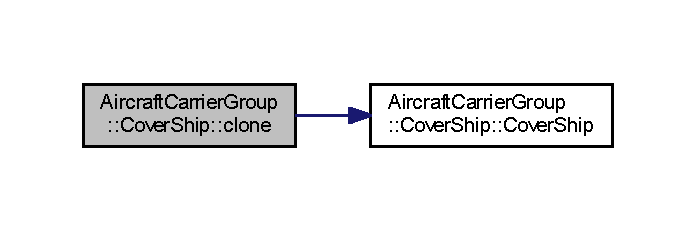
\includegraphics[width=334pt]{class_aircraft_carrier_group_1_1_cover_ship_aa6a5b007f5e05f9ad5cc300b8958309a_cgraph}
\end{center}
\end{figure}
\mbox{\Hypertarget{class_aircraft_carrier_group_1_1_cover_ship_a3a08ec471959146e36e3d6c2fccf2159}\label{class_aircraft_carrier_group_1_1_cover_ship_a3a08ec471959146e36e3d6c2fccf2159}} 
\index{Aircraft\+Carrier\+Group\+::\+Cover\+Ship@{Aircraft\+Carrier\+Group\+::\+Cover\+Ship}!Damage\+All\+Planes@{Damage\+All\+Planes}}
\index{Damage\+All\+Planes@{Damage\+All\+Planes}!Aircraft\+Carrier\+Group\+::\+Cover\+Ship@{Aircraft\+Carrier\+Group\+::\+Cover\+Ship}}
\subsubsection{\texorpdfstring{Damage\+All\+Planes()}{DamageAllPlanes()}}
{\footnotesize\ttfamily int Aircraft\+Carrier\+Group\+::\+Cover\+Ship\+::\+Damage\+All\+Planes (\begin{DoxyParamCaption}{ }\end{DoxyParamCaption}) const\hspace{0.3cm}{\ttfamily [inline]}, {\ttfamily [virtual]}}



Производит расчет разрушений, которые могут нанести все самолеты судна условной цели за единицу времени 


\begin{DoxyExceptions}{Exceptions}
{\em Invalid\+Ship\+Type} & При попытке рассчета урона всеми самолетам по условным целям, поскольку этот тип кораблей не может иметь самолетов на палубе \\
\hline
\end{DoxyExceptions}


Implements \mbox{\hyperlink{class_aircraft_carrier_group_1_1_ship_a2731c146c8edfc3a799661d249ccf522}{Aircraft\+Carrier\+Group\+::\+Ship}}.

\mbox{\Hypertarget{class_aircraft_carrier_group_1_1_cover_ship_ab587c598ab12561d4ecad32c5f55a04e}\label{class_aircraft_carrier_group_1_1_cover_ship_ab587c598ab12561d4ecad32c5f55a04e}} 
\index{Aircraft\+Carrier\+Group\+::\+Cover\+Ship@{Aircraft\+Carrier\+Group\+::\+Cover\+Ship}!get\+Weapon@{get\+Weapon}}
\index{get\+Weapon@{get\+Weapon}!Aircraft\+Carrier\+Group\+::\+Cover\+Ship@{Aircraft\+Carrier\+Group\+::\+Cover\+Ship}}
\subsubsection{\texorpdfstring{get\+Weapon()}{getWeapon()}}
{\footnotesize\ttfamily \mbox{\hyperlink{class_aircraft_carrier_group_1_1_weapon}{Weapon}} $\ast$ Aircraft\+Carrier\+Group\+::\+Cover\+Ship\+::get\+Weapon (\begin{DoxyParamCaption}\item[{std\+::string}]{Name }\end{DoxyParamCaption}) const\hspace{0.3cm}{\ttfamily [virtual]}}



Функция получает описатель оружия по его названию 


\begin{DoxyParams}{Parameters}
{\em Name} & Название оружия \\
\hline
\end{DoxyParams}
\begin{DoxyReturn}{Returns}
Возвращает указатель на область памяти, в котором хранится описатель найденного оружия 
\end{DoxyReturn}


Implements \mbox{\hyperlink{class_aircraft_carrier_group_1_1_ship_a8ac6e8e9ed4f997a5f02fda7e049cd6d}{Aircraft\+Carrier\+Group\+::\+Ship}}.

\mbox{\Hypertarget{class_aircraft_carrier_group_1_1_cover_ship_a135b4e20acbdb6bfbcb2cbb6df855d09}\label{class_aircraft_carrier_group_1_1_cover_ship_a135b4e20acbdb6bfbcb2cbb6df855d09}} 
\index{Aircraft\+Carrier\+Group\+::\+Cover\+Ship@{Aircraft\+Carrier\+Group\+::\+Cover\+Ship}!Weapon\+Modification@{Weapon\+Modification}}
\index{Weapon\+Modification@{Weapon\+Modification}!Aircraft\+Carrier\+Group\+::\+Cover\+Ship@{Aircraft\+Carrier\+Group\+::\+Cover\+Ship}}
\subsubsection{\texorpdfstring{Weapon\+Modification()}{WeaponModification()}}
{\footnotesize\ttfamily \mbox{\hyperlink{class_aircraft_carrier_group_1_1_cover_ship}{Cover\+Ship}} \& Aircraft\+Carrier\+Group\+::\+Cover\+Ship\+::\+Weapon\+Modification (\begin{DoxyParamCaption}\item[{std\+::string}]{Name\+Weapon\+Tmp,  }\item[{const \mbox{\hyperlink{class_aircraft_carrier_group_1_1_weapon}{Weapon}} \&}]{Weapon\+Tmp }\end{DoxyParamCaption})\hspace{0.3cm}{\ttfamily [virtual]}}



Функция модифицирует выбранное, из имеющихся на корабле, орудие 


\begin{DoxyParams}{Parameters}
{\em Name\+Weapon\+Tmp} & Названия орудия, которое надо модифицировать \\
\hline
{\em Weapon\+Tmp} & Новое орудие \\
\hline
\end{DoxyParams}


Implements \mbox{\hyperlink{class_aircraft_carrier_group_1_1_ship_a3f91c1ad2960c095cfd88e85df0a3990}{Aircraft\+Carrier\+Group\+::\+Ship}}.



The documentation for this class was generated from the following files\+:\begin{DoxyCompactItemize}
\item 
C\+:/\+Users/\+Sema/\+Desktop/\+Code\+Forces/\+Labs/4th\+\_\+\+Lab + library connection/\+Library/\mbox{\hyperlink{_cover_ship_8h}{Cover\+Ship.\+h}}\item 
C\+:/\+Users/\+Sema/\+Desktop/\+Code\+Forces/\+Labs/4th\+\_\+\+Lab + library connection/\+Library/Cover\+Ship.\+cpp\end{DoxyCompactItemize}

\hypertarget{class_aircraft_carrier_group_1_1_fleet}{}\section{Aircraft\+Carrier\+Group\+:\+:Fleet Class Reference}
\label{class_aircraft_carrier_group_1_1_fleet}\index{Aircraft\+Carrier\+Group\+::\+Fleet@{Aircraft\+Carrier\+Group\+::\+Fleet}}


Класс для описания флота  Осуществляет хранение описателей всех кораблей флота и содержит функции, позволяющие взаимодействовать с кораблями флота  




{\ttfamily \#include $<$Fleet.\+h$>$}

\subsection*{Public Types}
\begin{DoxyCompactItemize}
\item 
\mbox{\Hypertarget{class_aircraft_carrier_group_1_1_fleet_acf50fa081cc25e4a7a688d47797ccce7}\label{class_aircraft_carrier_group_1_1_fleet_acf50fa081cc25e4a7a688d47797ccce7}} 
typedef \mbox{\hyperlink{class_aircraft_carrier_group_1_1_const_fleet_it}{Const\+Fleet\+It}} {\bfseries Const\+\_\+\+Iterator}
\end{DoxyCompactItemize}
\subsection*{Public Member Functions}
\begin{DoxyCompactItemize}
\item 
\mbox{\Hypertarget{class_aircraft_carrier_group_1_1_fleet_a2ef466460d466153291eb4a4b62990a2}\label{class_aircraft_carrier_group_1_1_fleet_a2ef466460d466153291eb4a4b62990a2}} 
\mbox{\hyperlink{class_aircraft_carrier_group_1_1_fleet_a2ef466460d466153291eb4a4b62990a2}{Fleet}} ()
\begin{DoxyCompactList}\small\item\em Конструктор по умолчанию \end{DoxyCompactList}\item 
\mbox{\hyperlink{class_aircraft_carrier_group_1_1_fleet_afd8802987a6ff91b25cba30a140cc57a}{Fleet}} (const \mbox{\hyperlink{class_aircraft_carrier_group_1_1_fleet}{Fleet}} \&Navy)
\begin{DoxyCompactList}\small\item\em Копирующий конструктор \end{DoxyCompactList}\item 
\mbox{\Hypertarget{class_aircraft_carrier_group_1_1_fleet_a8468d2f43ed82a39a8e885168626a5dd}\label{class_aircraft_carrier_group_1_1_fleet_a8468d2f43ed82a39a8e885168626a5dd}} 
\mbox{\hyperlink{class_aircraft_carrier_group_1_1_fleet_a8468d2f43ed82a39a8e885168626a5dd}{$\sim$\+Fleet}} ()
\begin{DoxyCompactList}\small\item\em Деструктор \end{DoxyCompactList}\item 
\mbox{\Hypertarget{class_aircraft_carrier_group_1_1_fleet_aac2a2f25ae1967ba39ab3334da38bb5c}\label{class_aircraft_carrier_group_1_1_fleet_aac2a2f25ae1967ba39ab3334da38bb5c}} 
\mbox{\hyperlink{class_aircraft_carrier_group_1_1_const_fleet_it}{Const\+\_\+\+Iterator}} {\bfseries find} (const std\+::string \&) const
\item 
\mbox{\Hypertarget{class_aircraft_carrier_group_1_1_fleet_a239804d29253792f1abbc011ee752d63}\label{class_aircraft_carrier_group_1_1_fleet_a239804d29253792f1abbc011ee752d63}} 
\mbox{\hyperlink{class_aircraft_carrier_group_1_1_const_fleet_it}{Const\+\_\+\+Iterator}} {\bfseries begin} () const
\item 
\mbox{\Hypertarget{class_aircraft_carrier_group_1_1_fleet_ae0f445f9309b45e53a70cde913ab1192}\label{class_aircraft_carrier_group_1_1_fleet_ae0f445f9309b45e53a70cde913ab1192}} 
\mbox{\hyperlink{class_aircraft_carrier_group_1_1_const_fleet_it}{Const\+\_\+\+Iterator}} {\bfseries end} () const
\item 
\mbox{\Hypertarget{class_aircraft_carrier_group_1_1_fleet_a410acdddcd290d3c0760b895cd1210f7}\label{class_aircraft_carrier_group_1_1_fleet_a410acdddcd290d3c0760b895cd1210f7}} 
int \mbox{\hyperlink{class_aircraft_carrier_group_1_1_fleet_a410acdddcd290d3c0760b895cd1210f7}{Size\+Fleet}} () const
\begin{DoxyCompactList}\small\item\em Возвращает количество кораблей во флоте \end{DoxyCompactList}\item 
bool \mbox{\hyperlink{class_aircraft_carrier_group_1_1_fleet_ac2f313e4be33de186169699fe37163ab}{insert}} (std\+::string \&Call\+Tmp, \mbox{\hyperlink{class_aircraft_carrier_group_1_1_ship}{Ship}} $\ast$Ship\+Tmp)
\begin{DoxyCompactList}\small\item\em Добавляет новый корабль во флот \end{DoxyCompactList}\item 
bool \mbox{\hyperlink{class_aircraft_carrier_group_1_1_fleet_a7fa09607af647d0fb7edce10b90d28a3}{remove}} (std\+::string \&Call\+Tmp)
\begin{DoxyCompactList}\small\item\em Удаляет корабль из флота \end{DoxyCompactList}\item 
int \mbox{\hyperlink{class_aircraft_carrier_group_1_1_fleet_af9ddb1220e3a01986eaa433e52fa7098}{transfer\+Fuel}} (\mbox{\hyperlink{class_aircraft_carrier_group_1_1_const_fleet_it}{Fleet\+::\+Const\+\_\+\+Iterator}} \&it\+Fr, \mbox{\hyperlink{class_aircraft_carrier_group_1_1_const_fleet_it}{Fleet\+::\+Const\+\_\+\+Iterator}} \&it\+To, const int Fuel)
\begin{DoxyCompactList}\small\item\em Осуществляет перенос топлива с одного корабля на другой \end{DoxyCompactList}\item 
\mbox{\Hypertarget{class_aircraft_carrier_group_1_1_fleet_a3dc50b9a6145d8433c3d902f7dddf739}\label{class_aircraft_carrier_group_1_1_fleet_a3dc50b9a6145d8433c3d902f7dddf739}} 
int \mbox{\hyperlink{class_aircraft_carrier_group_1_1_fleet_a3dc50b9a6145d8433c3d902f7dddf739}{Type\+Cover\+Ship}} ()
\begin{DoxyCompactList}\small\item\em Возвращает количество кораблей прикрытия в группе \end{DoxyCompactList}\item 
\mbox{\Hypertarget{class_aircraft_carrier_group_1_1_fleet_a0c5184e9f603c11e58c68ab34f0d0a30}\label{class_aircraft_carrier_group_1_1_fleet_a0c5184e9f603c11e58c68ab34f0d0a30}} 
int \mbox{\hyperlink{class_aircraft_carrier_group_1_1_fleet_a0c5184e9f603c11e58c68ab34f0d0a30}{Type\+Carrier}} ()
\begin{DoxyCompactList}\small\item\em Возвращает количество авианесущих кораблей в группе \end{DoxyCompactList}\item 
\mbox{\Hypertarget{class_aircraft_carrier_group_1_1_fleet_a2ebc181699850e8bff283a281c22ea2b}\label{class_aircraft_carrier_group_1_1_fleet_a2ebc181699850e8bff283a281c22ea2b}} 
int \mbox{\hyperlink{class_aircraft_carrier_group_1_1_fleet_a2ebc181699850e8bff283a281c22ea2b}{Type\+Aircraft\+Carrier}} ()
\begin{DoxyCompactList}\small\item\em Возвращает количество авианесущих крейсеров в группе \end{DoxyCompactList}\item 
bool \mbox{\hyperlink{class_aircraft_carrier_group_1_1_fleet_af7863ad9b057b0212b04019956254e8a}{Add\+Plane}} (const \mbox{\hyperlink{class_aircraft_carrier_group_1_1_aircraft}{Aircraft}} \&Plane, const std\+::string \&Ship\+Tmp)
\begin{DoxyCompactList}\small\item\em Добавление самолета в авианесущую группу \end{DoxyCompactList}\item 
bool \mbox{\hyperlink{class_aircraft_carrier_group_1_1_fleet_aa464eecb22e71128b6a01733d71fc27e}{Delete\+Plane}} (const std\+::string \&Ship\+Tmp)
\begin{DoxyCompactList}\small\item\em Удаление самолета с корабля \end{DoxyCompactList}\item 
\mbox{\Hypertarget{class_aircraft_carrier_group_1_1_fleet_a3f8d69e2180159e964feb3ec41d442ee}\label{class_aircraft_carrier_group_1_1_fleet_a3f8d69e2180159e964feb3ec41d442ee}} 
double \mbox{\hyperlink{class_aircraft_carrier_group_1_1_fleet_a3f8d69e2180159e964feb3ec41d442ee}{Max\+Duration\+Plane\+Fligth}} ()
\begin{DoxyCompactList}\small\item\em Производит рассчет максимального времени полета всех самолетов авиагруппы \end{DoxyCompactList}\item 
\mbox{\Hypertarget{class_aircraft_carrier_group_1_1_fleet_ad36b1f4f06ac7f267e61d7fed71c04ff}\label{class_aircraft_carrier_group_1_1_fleet_ad36b1f4f06ac7f267e61d7fed71c04ff}} 
double \mbox{\hyperlink{class_aircraft_carrier_group_1_1_fleet_ad36b1f4f06ac7f267e61d7fed71c04ff}{Max\+Radius\+Plane\+Fligth}} ()
\begin{DoxyCompactList}\small\item\em Производит рассчет максимального радуса полета всех самолетов авиагруппы \end{DoxyCompactList}\item 
int \mbox{\hyperlink{class_aircraft_carrier_group_1_1_fleet_afdc755fad8b201aa497161a5ef63a97c}{Transfer\+Aircraft}} (\mbox{\hyperlink{class_aircraft_carrier_group_1_1_const_fleet_it}{Fleet\+::\+Const\+\_\+\+Iterator}} \&From, \mbox{\hyperlink{class_aircraft_carrier_group_1_1_const_fleet_it}{Fleet\+::\+Const\+\_\+\+Iterator}} \&To)
\begin{DoxyCompactList}\small\item\em Осуществляет перенос самолета с одного корабля на другой \end{DoxyCompactList}\item 
\mbox{\Hypertarget{class_aircraft_carrier_group_1_1_fleet_abe8311c40460ab1a8d32d9825980ca8a}\label{class_aircraft_carrier_group_1_1_fleet_abe8311c40460ab1a8d32d9825980ca8a}} 
void \mbox{\hyperlink{class_aircraft_carrier_group_1_1_fleet_abe8311c40460ab1a8d32d9825980ca8a}{clear}} ()
\begin{DoxyCompactList}\small\item\em Очистка контейнера, в котором хранится информация обо всех кораблях авианесущей группы \end{DoxyCompactList}\item 
\mbox{\Hypertarget{class_aircraft_carrier_group_1_1_fleet_a34d66ddac9b45d0b64202486ed484074}\label{class_aircraft_carrier_group_1_1_fleet_a34d66ddac9b45d0b64202486ed484074}} 
void \mbox{\hyperlink{class_aircraft_carrier_group_1_1_fleet_a34d66ddac9b45d0b64202486ed484074}{Show}} ()
\begin{DoxyCompactList}\small\item\em Вывод информации обо всех кораблях флота \end{DoxyCompactList}\item 
\mbox{\Hypertarget{class_aircraft_carrier_group_1_1_fleet_aaa91e21c9a4b9c56d3bb5e57a92bb464}\label{class_aircraft_carrier_group_1_1_fleet_aaa91e21c9a4b9c56d3bb5e57a92bb464}} 
\mbox{\hyperlink{class_aircraft_carrier_group_1_1_fleet}{Fleet}} \& {\bfseries operator=} (const \mbox{\hyperlink{class_aircraft_carrier_group_1_1_fleet}{Fleet}} \&)
\end{DoxyCompactItemize}
\subsection*{Friends}
\begin{DoxyCompactItemize}
\item 
\mbox{\Hypertarget{class_aircraft_carrier_group_1_1_fleet_ab159448042fb03231f44572ef8fd8075}\label{class_aircraft_carrier_group_1_1_fleet_ab159448042fb03231f44572ef8fd8075}} 
class {\bfseries Const\+Fleet\+It}
\item 
\mbox{\Hypertarget{class_aircraft_carrier_group_1_1_fleet_a21e2b274d6ab3bd444ecfeab143cd7e2}\label{class_aircraft_carrier_group_1_1_fleet_a21e2b274d6ab3bd444ecfeab143cd7e2}} 
std\+::ostream \& {\bfseries operator$<$$<$} (std\+::ostream \&, const \mbox{\hyperlink{class_aircraft_carrier_group_1_1_fleet}{Fleet}} \&)
\item 
\mbox{\Hypertarget{class_aircraft_carrier_group_1_1_fleet_ab81d2a31c8119517e381beab290f58fa}\label{class_aircraft_carrier_group_1_1_fleet_ab81d2a31c8119517e381beab290f58fa}} 
std\+::ifstream \& {\bfseries operator$>$$>$} (std\+::ifstream \&, \mbox{\hyperlink{class_aircraft_carrier_group_1_1_fleet}{Fleet}} \&)
\item 
\mbox{\Hypertarget{class_aircraft_carrier_group_1_1_fleet_ace3fe0aa2dcee997b91fddf929e4f021}\label{class_aircraft_carrier_group_1_1_fleet_ace3fe0aa2dcee997b91fddf929e4f021}} 
std\+::ofstream \& {\bfseries operator$<$$<$} (std\+::ofstream \&, const \mbox{\hyperlink{class_aircraft_carrier_group_1_1_fleet}{Fleet}} \&)
\end{DoxyCompactItemize}


\subsection{Detailed Description}
Класс для описания флота  Осуществляет хранение описателей всех кораблей флота и содержит функции, позволяющие взаимодействовать с кораблями флота 

\subsection{Constructor \& Destructor Documentation}
\mbox{\Hypertarget{class_aircraft_carrier_group_1_1_fleet_afd8802987a6ff91b25cba30a140cc57a}\label{class_aircraft_carrier_group_1_1_fleet_afd8802987a6ff91b25cba30a140cc57a}} 
\index{Aircraft\+Carrier\+Group\+::\+Fleet@{Aircraft\+Carrier\+Group\+::\+Fleet}!Fleet@{Fleet}}
\index{Fleet@{Fleet}!Aircraft\+Carrier\+Group\+::\+Fleet@{Aircraft\+Carrier\+Group\+::\+Fleet}}
\subsubsection{\texorpdfstring{Fleet()}{Fleet()}}
{\footnotesize\ttfamily Aircraft\+Carrier\+Group\+::\+Fleet\+::\+Fleet (\begin{DoxyParamCaption}\item[{const \mbox{\hyperlink{class_aircraft_carrier_group_1_1_fleet}{Fleet}} \&}]{Navy }\end{DoxyParamCaption})}



Копирующий конструктор 


\begin{DoxyParams}{Parameters}
{\em Cover\+Ship\+Tmp} & Описатель корабля прикрытия \\
\hline
\end{DoxyParams}


\subsection{Member Function Documentation}
\mbox{\Hypertarget{class_aircraft_carrier_group_1_1_fleet_af7863ad9b057b0212b04019956254e8a}\label{class_aircraft_carrier_group_1_1_fleet_af7863ad9b057b0212b04019956254e8a}} 
\index{Aircraft\+Carrier\+Group\+::\+Fleet@{Aircraft\+Carrier\+Group\+::\+Fleet}!Add\+Plane@{Add\+Plane}}
\index{Add\+Plane@{Add\+Plane}!Aircraft\+Carrier\+Group\+::\+Fleet@{Aircraft\+Carrier\+Group\+::\+Fleet}}
\subsubsection{\texorpdfstring{Add\+Plane()}{AddPlane()}}
{\footnotesize\ttfamily bool Aircraft\+Carrier\+Group\+::\+Fleet\+::\+Add\+Plane (\begin{DoxyParamCaption}\item[{const \mbox{\hyperlink{class_aircraft_carrier_group_1_1_aircraft}{Aircraft}} \&}]{Plane,  }\item[{const std\+::string \&}]{Ship\+Tmp }\end{DoxyParamCaption})}



Добавление самолета в авианесущую группу 


\begin{DoxyParams}{Parameters}
{\em Plane} & Самолет, информацию о котором необходимо внести в группу \\
\hline
{\em Ship\+Tmp} & Корабль, на который будет добавляться самолте \\
\hline
\end{DoxyParams}
Here is the call graph for this function\+:
\nopagebreak
\begin{figure}[H]
\begin{center}
\leavevmode
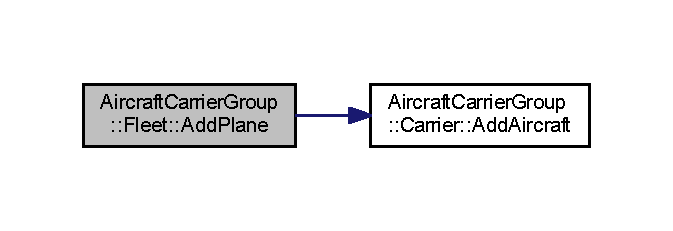
\includegraphics[width=323pt]{class_aircraft_carrier_group_1_1_fleet_af7863ad9b057b0212b04019956254e8a_cgraph}
\end{center}
\end{figure}
\mbox{\Hypertarget{class_aircraft_carrier_group_1_1_fleet_aa464eecb22e71128b6a01733d71fc27e}\label{class_aircraft_carrier_group_1_1_fleet_aa464eecb22e71128b6a01733d71fc27e}} 
\index{Aircraft\+Carrier\+Group\+::\+Fleet@{Aircraft\+Carrier\+Group\+::\+Fleet}!Delete\+Plane@{Delete\+Plane}}
\index{Delete\+Plane@{Delete\+Plane}!Aircraft\+Carrier\+Group\+::\+Fleet@{Aircraft\+Carrier\+Group\+::\+Fleet}}
\subsubsection{\texorpdfstring{Delete\+Plane()}{DeletePlane()}}
{\footnotesize\ttfamily bool Aircraft\+Carrier\+Group\+::\+Fleet\+::\+Delete\+Plane (\begin{DoxyParamCaption}\item[{const std\+::string \&}]{Ship\+Tmp }\end{DoxyParamCaption})}



Удаление самолета с корабля 


\begin{DoxyParams}{Parameters}
{\em Ship\+Tmp} & Корабль, с которого будет производиться удаление самолета \\
\hline
\end{DoxyParams}
Here is the call graph for this function\+:
\nopagebreak
\begin{figure}[H]
\begin{center}
\leavevmode
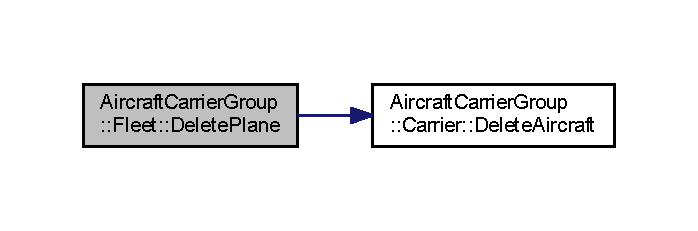
\includegraphics[width=335pt]{class_aircraft_carrier_group_1_1_fleet_aa464eecb22e71128b6a01733d71fc27e_cgraph}
\end{center}
\end{figure}
\mbox{\Hypertarget{class_aircraft_carrier_group_1_1_fleet_ac2f313e4be33de186169699fe37163ab}\label{class_aircraft_carrier_group_1_1_fleet_ac2f313e4be33de186169699fe37163ab}} 
\index{Aircraft\+Carrier\+Group\+::\+Fleet@{Aircraft\+Carrier\+Group\+::\+Fleet}!insert@{insert}}
\index{insert@{insert}!Aircraft\+Carrier\+Group\+::\+Fleet@{Aircraft\+Carrier\+Group\+::\+Fleet}}
\subsubsection{\texorpdfstring{insert()}{insert()}}
{\footnotesize\ttfamily bool Aircraft\+Carrier\+Group\+::\+Fleet\+::insert (\begin{DoxyParamCaption}\item[{std\+::string \&}]{Call\+Tmp,  }\item[{\mbox{\hyperlink{class_aircraft_carrier_group_1_1_ship}{Ship}} $\ast$}]{Ship\+Tmp }\end{DoxyParamCaption})}



Добавляет новый корабль во флот 


\begin{DoxyParams}{Parameters}
{\em Call\+Tmp} & Позывной нового корабля \\
\hline
{\em Ship\+Tmp} & Указатель на область памяти, в котором хранится вся информация о корабле \\
\hline
\end{DoxyParams}
Here is the call graph for this function\+:
\nopagebreak
\begin{figure}[H]
\begin{center}
\leavevmode
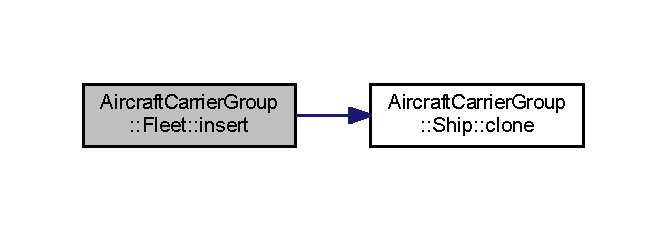
\includegraphics[width=320pt]{class_aircraft_carrier_group_1_1_fleet_ac2f313e4be33de186169699fe37163ab_cgraph}
\end{center}
\end{figure}
\mbox{\Hypertarget{class_aircraft_carrier_group_1_1_fleet_a7fa09607af647d0fb7edce10b90d28a3}\label{class_aircraft_carrier_group_1_1_fleet_a7fa09607af647d0fb7edce10b90d28a3}} 
\index{Aircraft\+Carrier\+Group\+::\+Fleet@{Aircraft\+Carrier\+Group\+::\+Fleet}!remove@{remove}}
\index{remove@{remove}!Aircraft\+Carrier\+Group\+::\+Fleet@{Aircraft\+Carrier\+Group\+::\+Fleet}}
\subsubsection{\texorpdfstring{remove()}{remove()}}
{\footnotesize\ttfamily bool Aircraft\+Carrier\+Group\+::\+Fleet\+::remove (\begin{DoxyParamCaption}\item[{std\+::string \&}]{Call\+Tmp }\end{DoxyParamCaption})}



Удаляет корабль из флота 


\begin{DoxyParams}{Parameters}
{\em Call\+Tmp} & Позывной удаляемого корабля \\
\hline
\end{DoxyParams}
\mbox{\Hypertarget{class_aircraft_carrier_group_1_1_fleet_afdc755fad8b201aa497161a5ef63a97c}\label{class_aircraft_carrier_group_1_1_fleet_afdc755fad8b201aa497161a5ef63a97c}} 
\index{Aircraft\+Carrier\+Group\+::\+Fleet@{Aircraft\+Carrier\+Group\+::\+Fleet}!Transfer\+Aircraft@{Transfer\+Aircraft}}
\index{Transfer\+Aircraft@{Transfer\+Aircraft}!Aircraft\+Carrier\+Group\+::\+Fleet@{Aircraft\+Carrier\+Group\+::\+Fleet}}
\subsubsection{\texorpdfstring{Transfer\+Aircraft()}{TransferAircraft()}}
{\footnotesize\ttfamily int Aircraft\+Carrier\+Group\+::\+Fleet\+::\+Transfer\+Aircraft (\begin{DoxyParamCaption}\item[{\mbox{\hyperlink{class_aircraft_carrier_group_1_1_const_fleet_it}{Fleet\+::\+Const\+\_\+\+Iterator}} \&}]{From,  }\item[{\mbox{\hyperlink{class_aircraft_carrier_group_1_1_const_fleet_it}{Fleet\+::\+Const\+\_\+\+Iterator}} \&}]{To }\end{DoxyParamCaption})}



Осуществляет перенос самолета с одного корабля на другой 


\begin{DoxyParams}{Parameters}
{\em From} & Корабль, с которого берется самолет \\
\hline
{\em To} & Корабль, на который переносится самолет \\
\hline
\end{DoxyParams}
Here is the call graph for this function\+:
\nopagebreak
\begin{figure}[H]
\begin{center}
\leavevmode
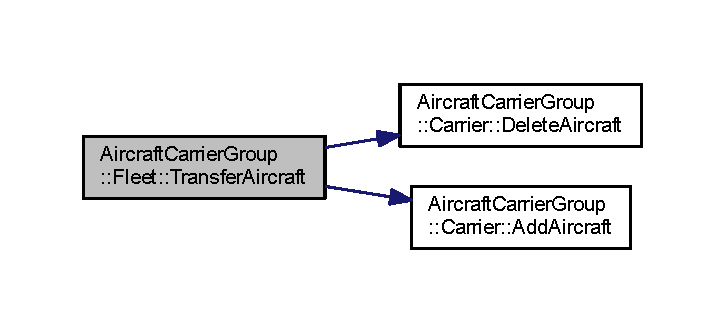
\includegraphics[width=348pt]{class_aircraft_carrier_group_1_1_fleet_afdc755fad8b201aa497161a5ef63a97c_cgraph}
\end{center}
\end{figure}
\mbox{\Hypertarget{class_aircraft_carrier_group_1_1_fleet_af9ddb1220e3a01986eaa433e52fa7098}\label{class_aircraft_carrier_group_1_1_fleet_af9ddb1220e3a01986eaa433e52fa7098}} 
\index{Aircraft\+Carrier\+Group\+::\+Fleet@{Aircraft\+Carrier\+Group\+::\+Fleet}!transfer\+Fuel@{transfer\+Fuel}}
\index{transfer\+Fuel@{transfer\+Fuel}!Aircraft\+Carrier\+Group\+::\+Fleet@{Aircraft\+Carrier\+Group\+::\+Fleet}}
\subsubsection{\texorpdfstring{transfer\+Fuel()}{transferFuel()}}
{\footnotesize\ttfamily int Aircraft\+Carrier\+Group\+::\+Fleet\+::transfer\+Fuel (\begin{DoxyParamCaption}\item[{\mbox{\hyperlink{class_aircraft_carrier_group_1_1_const_fleet_it}{Fleet\+::\+Const\+\_\+\+Iterator}} \&}]{it\+Fr,  }\item[{\mbox{\hyperlink{class_aircraft_carrier_group_1_1_const_fleet_it}{Fleet\+::\+Const\+\_\+\+Iterator}} \&}]{it\+To,  }\item[{const int}]{Fuel }\end{DoxyParamCaption})}



Осуществляет перенос топлива с одного корабля на другой 


\begin{DoxyParams}{Parameters}
{\em it\+Fr} & Корабль, с которого берется топливо \\
\hline
{\em it\+To} & Корабль, на который переносится топливо \\
\hline
{\em Fuel} & Количество топлива, которое необходимо перенести \\
\hline
\end{DoxyParams}


The documentation for this class was generated from the following files\+:\begin{DoxyCompactItemize}
\item 
C\+:/\+Users/\+Sema/\+Desktop/\+Code\+Forces/\+Labs/4th\+\_\+\+Lab + library connection/\+Library/\mbox{\hyperlink{_fleet_8h}{Fleet.\+h}}\item 
C\+:/\+Users/\+Sema/\+Desktop/\+Code\+Forces/\+Labs/4th\+\_\+\+Lab + library connection/\+Library/Fleet.\+cpp\end{DoxyCompactItemize}

\hypertarget{class_aircraft_carrier_group_1_1_military_characteristics}{}\section{Aircraft\+Carrier\+Group\+:\+:Military\+Characteristics Class Reference}
\label{class_aircraft_carrier_group_1_1_military_characteristics}\index{Aircraft\+Carrier\+Group\+::\+Military\+Characteristics@{Aircraft\+Carrier\+Group\+::\+Military\+Characteristics}}


Класс для описания некоторых парметров техники  Осуществляет хранение и обработку некоторых характеристик техники  




{\ttfamily \#include $<$Military\+Characteristics.\+h$>$}



Inheritance diagram for Aircraft\+Carrier\+Group\+:\+:Military\+Characteristics\+:
\nopagebreak
\begin{figure}[H]
\begin{center}
\leavevmode
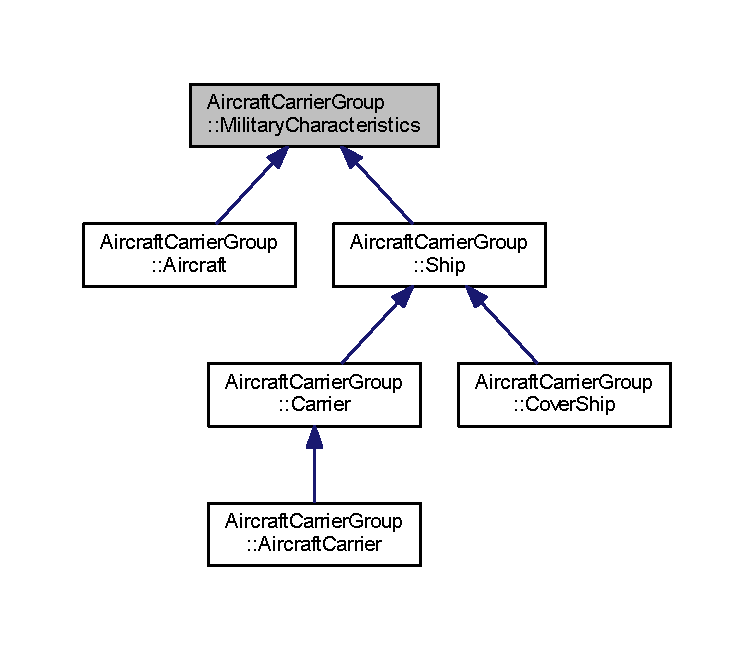
\includegraphics[width=350pt]{class_aircraft_carrier_group_1_1_military_characteristics__inherit__graph}
\end{center}
\end{figure}
\subsection*{Public Member Functions}
\begin{DoxyCompactItemize}
\item 
\mbox{\Hypertarget{class_aircraft_carrier_group_1_1_military_characteristics_a43c76dd547a8abd8f0b43920e891744f}\label{class_aircraft_carrier_group_1_1_military_characteristics_a43c76dd547a8abd8f0b43920e891744f}} 
\mbox{\hyperlink{class_aircraft_carrier_group_1_1_military_characteristics_a43c76dd547a8abd8f0b43920e891744f}{Military\+Characteristics}} ()
\begin{DoxyCompactList}\small\item\em Конструктор по умолчанию \end{DoxyCompactList}\item 
\mbox{\hyperlink{class_aircraft_carrier_group_1_1_military_characteristics_a6bd6050279bfeb4b19a65521954a6fd3}{Military\+Characteristics}} (int Speed\+Tmp, int Fuel\+Consumption\+Tmp, int Fuel\+Reserve\+Tmp)
\begin{DoxyCompactList}\small\item\em Инициализирующий конструктор \end{DoxyCompactList}\item 
\mbox{\hyperlink{class_aircraft_carrier_group_1_1_military_characteristics_a3467139f8217e53800e8cb0f72fab64c}{Military\+Characteristics}} (const \mbox{\hyperlink{class_aircraft_carrier_group_1_1_military_characteristics}{Military\+Characteristics}} \&Military)
\begin{DoxyCompactList}\small\item\em Копирующий конструктор \end{DoxyCompactList}\item 
\mbox{\Hypertarget{class_aircraft_carrier_group_1_1_military_characteristics_adcbeb18ee8db4a3d9f6f858cdc974fc6}\label{class_aircraft_carrier_group_1_1_military_characteristics_adcbeb18ee8db4a3d9f6f858cdc974fc6}} 
virtual \mbox{\hyperlink{class_aircraft_carrier_group_1_1_military_characteristics_adcbeb18ee8db4a3d9f6f858cdc974fc6}{$\sim$\+Military\+Characteristics}} ()
\begin{DoxyCompactList}\small\item\em Деструктор \end{DoxyCompactList}\item 
\mbox{\hyperlink{class_aircraft_carrier_group_1_1_military_characteristics}{Military\+Characteristics}} \& \mbox{\hyperlink{class_aircraft_carrier_group_1_1_military_characteristics_a185dc7a09586db8136fccc33d6b22681}{Set\+Speed}} (int Speed\+Tmp)
\begin{DoxyCompactList}\small\item\em Устанавливает скорость техники \end{DoxyCompactList}\item 
\mbox{\hyperlink{class_aircraft_carrier_group_1_1_military_characteristics}{Military\+Characteristics}} \& \mbox{\hyperlink{class_aircraft_carrier_group_1_1_military_characteristics_a4a3a967ea54b0b01d40fb0ae2db01d14}{Set\+Fuel\+Reserve}} (int Fuel\+Reserve\+Tmp)
\begin{DoxyCompactList}\small\item\em Устанавливает запас топлива в технике \end{DoxyCompactList}\item 
\mbox{\hyperlink{class_aircraft_carrier_group_1_1_military_characteristics}{Military\+Characteristics}} \& \mbox{\hyperlink{class_aircraft_carrier_group_1_1_military_characteristics_a7963f5f29aa9b409819eeb976e0f3456}{Set\+Fuel\+Consumption}} (int Fuel\+Consumption\+Tmp)
\begin{DoxyCompactList}\small\item\em Устанавливает расход топлива в технике \end{DoxyCompactList}\item 
\mbox{\Hypertarget{class_aircraft_carrier_group_1_1_military_characteristics_a78e91ace73aa0e935bc258154d4a40b8}\label{class_aircraft_carrier_group_1_1_military_characteristics_a78e91ace73aa0e935bc258154d4a40b8}} 
int \mbox{\hyperlink{class_aircraft_carrier_group_1_1_military_characteristics_a78e91ace73aa0e935bc258154d4a40b8}{Get\+Speed}} () const
\begin{DoxyCompactList}\small\item\em Возвращает скорость техники \end{DoxyCompactList}\item 
\mbox{\Hypertarget{class_aircraft_carrier_group_1_1_military_characteristics_a4581672300228b600036a3fcc2f823e4}\label{class_aircraft_carrier_group_1_1_military_characteristics_a4581672300228b600036a3fcc2f823e4}} 
int \mbox{\hyperlink{class_aircraft_carrier_group_1_1_military_characteristics_a4581672300228b600036a3fcc2f823e4}{Get\+Fuel\+Reserve}} () const
\begin{DoxyCompactList}\small\item\em Возвращает запас топлива \end{DoxyCompactList}\item 
\mbox{\Hypertarget{class_aircraft_carrier_group_1_1_military_characteristics_aa7fe4f3183e2a0da56c381c1805cf8fa}\label{class_aircraft_carrier_group_1_1_military_characteristics_aa7fe4f3183e2a0da56c381c1805cf8fa}} 
int \mbox{\hyperlink{class_aircraft_carrier_group_1_1_military_characteristics_aa7fe4f3183e2a0da56c381c1805cf8fa}{Get\+Fuel\+Consumption}} () const
\begin{DoxyCompactList}\small\item\em Возвращает расход топлива \end{DoxyCompactList}\item 
\mbox{\Hypertarget{class_aircraft_carrier_group_1_1_military_characteristics_ad833de2850f537bf7d5e4479b611f215}\label{class_aircraft_carrier_group_1_1_military_characteristics_ad833de2850f537bf7d5e4479b611f215}} 
\mbox{\hyperlink{class_aircraft_carrier_group_1_1_military_characteristics}{Military\+Characteristics}} \& {\bfseries operator=} (const \mbox{\hyperlink{class_aircraft_carrier_group_1_1_military_characteristics}{Military\+Characteristics}} \&Military)
\item 
\mbox{\Hypertarget{class_aircraft_carrier_group_1_1_military_characteristics_a851be742216c85d487de56e2554b708e}\label{class_aircraft_carrier_group_1_1_military_characteristics_a851be742216c85d487de56e2554b708e}} 
\mbox{\hyperlink{class_aircraft_carrier_group_1_1_military_characteristics}{Military\+Characteristics}} \& {\bfseries operator=} (\mbox{\hyperlink{class_aircraft_carrier_group_1_1_military_characteristics}{Military\+Characteristics}} \&\&Military)
\end{DoxyCompactItemize}
\subsection*{Protected Attributes}
\begin{DoxyCompactItemize}
\item 
\mbox{\Hypertarget{class_aircraft_carrier_group_1_1_military_characteristics_a09676924ba08467f77d5607912294149}\label{class_aircraft_carrier_group_1_1_military_characteristics_a09676924ba08467f77d5607912294149}} 
int {\bfseries Speed}
\item 
\mbox{\Hypertarget{class_aircraft_carrier_group_1_1_military_characteristics_aee11eed2567d06ebd883612877bac252}\label{class_aircraft_carrier_group_1_1_military_characteristics_aee11eed2567d06ebd883612877bac252}} 
int {\bfseries Fuel\+Reserve}
\item 
\mbox{\Hypertarget{class_aircraft_carrier_group_1_1_military_characteristics_a669055459b6065f3ae138fa3f539aa56}\label{class_aircraft_carrier_group_1_1_military_characteristics_a669055459b6065f3ae138fa3f539aa56}} 
int {\bfseries Fuel\+Consumption}
\end{DoxyCompactItemize}
\subsection*{Friends}
\begin{DoxyCompactItemize}
\item 
\mbox{\Hypertarget{class_aircraft_carrier_group_1_1_military_characteristics_a41b44d946c935e5b0f2bf78e75cb079d}\label{class_aircraft_carrier_group_1_1_military_characteristics_a41b44d946c935e5b0f2bf78e75cb079d}} 
std\+::ostream \& {\bfseries operator$<$$<$} (std\+::ostream \&os, const \mbox{\hyperlink{class_aircraft_carrier_group_1_1_military_characteristics}{Military\+Characteristics}} \&Military)
\item 
\mbox{\Hypertarget{class_aircraft_carrier_group_1_1_military_characteristics_a9bf2dba162f5eb248157d479e26f1fa8}\label{class_aircraft_carrier_group_1_1_military_characteristics_a9bf2dba162f5eb248157d479e26f1fa8}} 
std\+::istream \& {\bfseries operator$>$$>$} (std\+::istream \&is, \mbox{\hyperlink{class_aircraft_carrier_group_1_1_military_characteristics}{Military\+Characteristics}} \&Military)
\item 
\mbox{\Hypertarget{class_aircraft_carrier_group_1_1_military_characteristics_acfb674eca6b7f8071cec488969f873ce}\label{class_aircraft_carrier_group_1_1_military_characteristics_acfb674eca6b7f8071cec488969f873ce}} 
std\+::ofstream \& {\bfseries operator$<$$<$} (std\+::ofstream \&os, const \mbox{\hyperlink{class_aircraft_carrier_group_1_1_military_characteristics}{Military\+Characteristics}} \&Military)
\item 
\mbox{\Hypertarget{class_aircraft_carrier_group_1_1_military_characteristics_a2deb6a3df02cd7aa1806b6d7c3396f5f}\label{class_aircraft_carrier_group_1_1_military_characteristics_a2deb6a3df02cd7aa1806b6d7c3396f5f}} 
std\+::ifstream \& {\bfseries operator$>$$>$} (std\+::ifstream \&is, \mbox{\hyperlink{class_aircraft_carrier_group_1_1_military_characteristics}{Military\+Characteristics}} \&Military)
\end{DoxyCompactItemize}


\subsection{Detailed Description}
Класс для описания некоторых парметров техники  Осуществляет хранение и обработку некоторых характеристик техники 

\subsection{Constructor \& Destructor Documentation}
\mbox{\Hypertarget{class_aircraft_carrier_group_1_1_military_characteristics_a6bd6050279bfeb4b19a65521954a6fd3}\label{class_aircraft_carrier_group_1_1_military_characteristics_a6bd6050279bfeb4b19a65521954a6fd3}} 
\index{Aircraft\+Carrier\+Group\+::\+Military\+Characteristics@{Aircraft\+Carrier\+Group\+::\+Military\+Characteristics}!Military\+Characteristics@{Military\+Characteristics}}
\index{Military\+Characteristics@{Military\+Characteristics}!Aircraft\+Carrier\+Group\+::\+Military\+Characteristics@{Aircraft\+Carrier\+Group\+::\+Military\+Characteristics}}
\subsubsection{\texorpdfstring{Military\+Characteristics()}{MilitaryCharacteristics()}\hspace{0.1cm}{\footnotesize\ttfamily [1/2]}}
{\footnotesize\ttfamily Aircraft\+Carrier\+Group\+::\+Military\+Characteristics\+::\+Military\+Characteristics (\begin{DoxyParamCaption}\item[{int}]{Speed\+Tmp,  }\item[{int}]{Fuel\+Consumption\+Tmp,  }\item[{int}]{Fuel\+Reserve\+Tmp = {\ttfamily 0} }\end{DoxyParamCaption})}



Инициализирующий конструктор 


\begin{DoxyParams}{Parameters}
{\em Speed\+Tmp} & Скорость \\
\hline
{\em Fuel\+Reserve\+Tmp} & Запас топлива \\
\hline
{\em Fuel\+Consumption\+Tmp} & Расход топлива \\
\hline
\end{DoxyParams}
\mbox{\Hypertarget{class_aircraft_carrier_group_1_1_military_characteristics_a3467139f8217e53800e8cb0f72fab64c}\label{class_aircraft_carrier_group_1_1_military_characteristics_a3467139f8217e53800e8cb0f72fab64c}} 
\index{Aircraft\+Carrier\+Group\+::\+Military\+Characteristics@{Aircraft\+Carrier\+Group\+::\+Military\+Characteristics}!Military\+Characteristics@{Military\+Characteristics}}
\index{Military\+Characteristics@{Military\+Characteristics}!Aircraft\+Carrier\+Group\+::\+Military\+Characteristics@{Aircraft\+Carrier\+Group\+::\+Military\+Characteristics}}
\subsubsection{\texorpdfstring{Military\+Characteristics()}{MilitaryCharacteristics()}\hspace{0.1cm}{\footnotesize\ttfamily [2/2]}}
{\footnotesize\ttfamily Aircraft\+Carrier\+Group\+::\+Military\+Characteristics\+::\+Military\+Characteristics (\begin{DoxyParamCaption}\item[{const \mbox{\hyperlink{class_aircraft_carrier_group_1_1_military_characteristics}{Military\+Characteristics}} \&}]{Military }\end{DoxyParamCaption})}



Копирующий конструктор 


\begin{DoxyParams}{Parameters}
{\em Military} & Объект класса, для которого будет произведено копирование \\
\hline
\end{DoxyParams}


\subsection{Member Function Documentation}
\mbox{\Hypertarget{class_aircraft_carrier_group_1_1_military_characteristics_a7963f5f29aa9b409819eeb976e0f3456}\label{class_aircraft_carrier_group_1_1_military_characteristics_a7963f5f29aa9b409819eeb976e0f3456}} 
\index{Aircraft\+Carrier\+Group\+::\+Military\+Characteristics@{Aircraft\+Carrier\+Group\+::\+Military\+Characteristics}!Set\+Fuel\+Consumption@{Set\+Fuel\+Consumption}}
\index{Set\+Fuel\+Consumption@{Set\+Fuel\+Consumption}!Aircraft\+Carrier\+Group\+::\+Military\+Characteristics@{Aircraft\+Carrier\+Group\+::\+Military\+Characteristics}}
\subsubsection{\texorpdfstring{Set\+Fuel\+Consumption()}{SetFuelConsumption()}}
{\footnotesize\ttfamily \mbox{\hyperlink{class_aircraft_carrier_group_1_1_military_characteristics}{Military\+Characteristics}}\& Aircraft\+Carrier\+Group\+::\+Military\+Characteristics\+::\+Set\+Fuel\+Consumption (\begin{DoxyParamCaption}\item[{int}]{Fuel\+Consumption\+Tmp }\end{DoxyParamCaption})\hspace{0.3cm}{\ttfamily [inline]}}



Устанавливает расход топлива в технике 


\begin{DoxyParams}[1]{Parameters}
\mbox{\tt in}  & {\em Fuel\+Consumption\+Tmp} & Запас топлива \\
\hline
\end{DoxyParams}
\begin{DoxyReturn}{Returns}
Возвращает измененные параметры техники 
\end{DoxyReturn}
\mbox{\Hypertarget{class_aircraft_carrier_group_1_1_military_characteristics_a4a3a967ea54b0b01d40fb0ae2db01d14}\label{class_aircraft_carrier_group_1_1_military_characteristics_a4a3a967ea54b0b01d40fb0ae2db01d14}} 
\index{Aircraft\+Carrier\+Group\+::\+Military\+Characteristics@{Aircraft\+Carrier\+Group\+::\+Military\+Characteristics}!Set\+Fuel\+Reserve@{Set\+Fuel\+Reserve}}
\index{Set\+Fuel\+Reserve@{Set\+Fuel\+Reserve}!Aircraft\+Carrier\+Group\+::\+Military\+Characteristics@{Aircraft\+Carrier\+Group\+::\+Military\+Characteristics}}
\subsubsection{\texorpdfstring{Set\+Fuel\+Reserve()}{SetFuelReserve()}}
{\footnotesize\ttfamily \mbox{\hyperlink{class_aircraft_carrier_group_1_1_military_characteristics}{Military\+Characteristics}}\& Aircraft\+Carrier\+Group\+::\+Military\+Characteristics\+::\+Set\+Fuel\+Reserve (\begin{DoxyParamCaption}\item[{int}]{Fuel\+Reserve\+Tmp }\end{DoxyParamCaption})\hspace{0.3cm}{\ttfamily [inline]}}



Устанавливает запас топлива в технике 


\begin{DoxyParams}[1]{Parameters}
\mbox{\tt in}  & {\em Fuel\+Reserve\+Tmp} & Запас топлива \\
\hline
\end{DoxyParams}
\begin{DoxyReturn}{Returns}
Возвращает измененные параметры техники 
\end{DoxyReturn}
\mbox{\Hypertarget{class_aircraft_carrier_group_1_1_military_characteristics_a185dc7a09586db8136fccc33d6b22681}\label{class_aircraft_carrier_group_1_1_military_characteristics_a185dc7a09586db8136fccc33d6b22681}} 
\index{Aircraft\+Carrier\+Group\+::\+Military\+Characteristics@{Aircraft\+Carrier\+Group\+::\+Military\+Characteristics}!Set\+Speed@{Set\+Speed}}
\index{Set\+Speed@{Set\+Speed}!Aircraft\+Carrier\+Group\+::\+Military\+Characteristics@{Aircraft\+Carrier\+Group\+::\+Military\+Characteristics}}
\subsubsection{\texorpdfstring{Set\+Speed()}{SetSpeed()}}
{\footnotesize\ttfamily \mbox{\hyperlink{class_aircraft_carrier_group_1_1_military_characteristics}{Military\+Characteristics}}\& Aircraft\+Carrier\+Group\+::\+Military\+Characteristics\+::\+Set\+Speed (\begin{DoxyParamCaption}\item[{int}]{Speed\+Tmp }\end{DoxyParamCaption})\hspace{0.3cm}{\ttfamily [inline]}}



Устанавливает скорость техники 


\begin{DoxyParams}[1]{Parameters}
\mbox{\tt in}  & {\em Speed\+Tmp} & Скорость, на которую нужно поменять \\
\hline
\end{DoxyParams}
\begin{DoxyReturn}{Returns}
Возвращает измененные параметры техники 
\end{DoxyReturn}


The documentation for this class was generated from the following files\+:\begin{DoxyCompactItemize}
\item 
C\+:/\+Users/\+Sema/\+Desktop/\+Code\+Forces/\+Labs/4th\+\_\+\+Lab + library connection/\+Library/\mbox{\hyperlink{_military_characteristics_8h}{Military\+Characteristics.\+h}}\item 
C\+:/\+Users/\+Sema/\+Desktop/\+Code\+Forces/\+Labs/4th\+\_\+\+Lab + library connection/\+Library/Military\+Characteristics.\+cpp\end{DoxyCompactItemize}

\hypertarget{class_aircraft_carrier_group_1_1_ship}{}\section{Aircraft\+Carrier\+Group\+:\+:Ship Class Reference}
\label{class_aircraft_carrier_group_1_1_ship}\index{Aircraft\+Carrier\+Group\+::\+Ship@{Aircraft\+Carrier\+Group\+::\+Ship}}


Абстрактный класс для описания кораблей  Осуществляет хранение общих параметров кораблей и содержит функции, обрабатывающие эти параметры  




{\ttfamily \#include $<$Ship.\+h$>$}



Inheritance diagram for Aircraft\+Carrier\+Group\+:\+:Ship\+:
\nopagebreak
\begin{figure}[H]
\begin{center}
\leavevmode
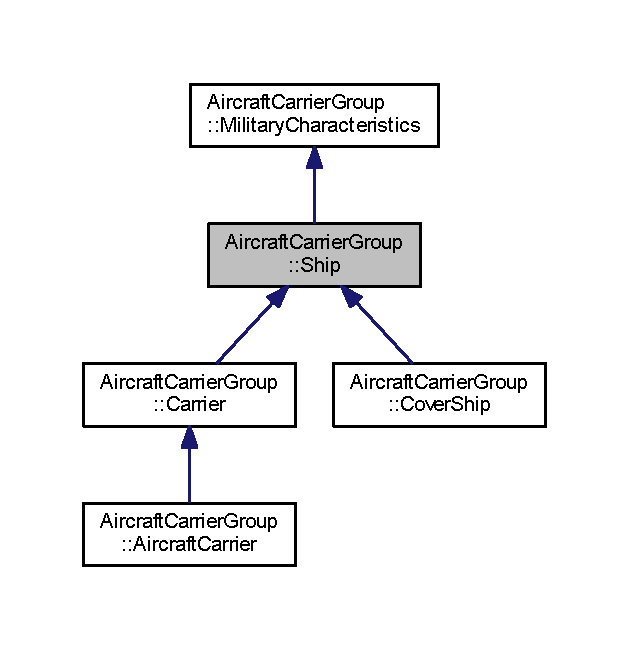
\includegraphics[width=302pt]{class_aircraft_carrier_group_1_1_ship__inherit__graph}
\end{center}
\end{figure}


Collaboration diagram for Aircraft\+Carrier\+Group\+:\+:Ship\+:
\nopagebreak
\begin{figure}[H]
\begin{center}
\leavevmode
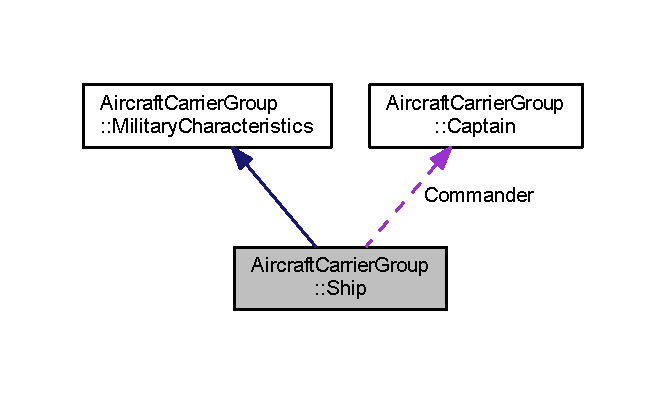
\includegraphics[width=320pt]{class_aircraft_carrier_group_1_1_ship__coll__graph}
\end{center}
\end{figure}
\subsection*{Public Member Functions}
\begin{DoxyCompactItemize}
\item 
\mbox{\Hypertarget{class_aircraft_carrier_group_1_1_ship_ab212e1c1cee164094489febc49bc7d65}\label{class_aircraft_carrier_group_1_1_ship_ab212e1c1cee164094489febc49bc7d65}} 
\mbox{\hyperlink{class_aircraft_carrier_group_1_1_ship_ab212e1c1cee164094489febc49bc7d65}{Ship}} ()
\begin{DoxyCompactList}\small\item\em Конструктор по умолчанию \end{DoxyCompactList}\item 
\mbox{\hyperlink{class_aircraft_carrier_group_1_1_ship_a1886e067969dae38d4a679de17f490fc}{Ship}} (std\+::string Call\+Tmp, const \mbox{\hyperlink{struct_aircraft_carrier_group_1_1_captain}{Captain}} \&Commander\+Tmp, int Crew\+Tmp, const \mbox{\hyperlink{class_aircraft_carrier_group_1_1_military_characteristics}{Military\+Characteristics}} \&Military\+Tmp)
\begin{DoxyCompactList}\small\item\em Инициализирующий конструктор \end{DoxyCompactList}\item 
\mbox{\hyperlink{class_aircraft_carrier_group_1_1_ship_a3465b634fa28d353509ea05a131d5af8}{Ship}} (std\+::string Call\+Tmp, std\+::string Name\+Tmp, std\+::string Rank\+Tmp, int Experience\+Tmp, int Crew\+Tmp, const \mbox{\hyperlink{class_aircraft_carrier_group_1_1_military_characteristics}{Military\+Characteristics}} \&Military\+Tmp)
\begin{DoxyCompactList}\small\item\em Инициализирующий конструктор \end{DoxyCompactList}\item 
\mbox{\hyperlink{class_aircraft_carrier_group_1_1_ship_ac6e81f533e9ee6165423668837cef5fd}{Ship}} (std\+::string Call\+Tmp, const \mbox{\hyperlink{struct_aircraft_carrier_group_1_1_captain}{Captain}} \&Commander\+Tmp, int Crew\+Tmp, int Speed\+Tmp, int Fuel\+Consumption\+Tmp, int Fuel\+Reserve\+Tmp)
\begin{DoxyCompactList}\small\item\em Инициализирующий конструктор \end{DoxyCompactList}\item 
\mbox{\hyperlink{class_aircraft_carrier_group_1_1_ship_ae4f36b334822955bfd4304835b9a7e7d}{Ship}} (std\+::string Call\+Tmp, std\+::string Name\+Tmp, std\+::string Rank\+Tmp, int Experience\+Tmp, int Crew\+Tmp, int Speed\+Tmp, int Fuel\+Consumption\+Tmp, int Fuel\+Reserve\+Tmp)
\begin{DoxyCompactList}\small\item\em Инициализирующий конструктор \end{DoxyCompactList}\item 
\mbox{\hyperlink{class_aircraft_carrier_group_1_1_ship_a55e9efaf784cdecbdd271bdda777fc21}{Ship}} (const \mbox{\hyperlink{class_aircraft_carrier_group_1_1_ship}{Ship}} \&Ship\+Tmp)
\begin{DoxyCompactList}\small\item\em Копирующий конструктор \end{DoxyCompactList}\item 
\mbox{\Hypertarget{class_aircraft_carrier_group_1_1_ship_acaa37cfea97f85bcf16221262aca593c}\label{class_aircraft_carrier_group_1_1_ship_acaa37cfea97f85bcf16221262aca593c}} 
virtual \mbox{\hyperlink{class_aircraft_carrier_group_1_1_ship_acaa37cfea97f85bcf16221262aca593c}{$\sim$\+Ship}} ()
\begin{DoxyCompactList}\small\item\em Деструктор \end{DoxyCompactList}\item 
\mbox{\hyperlink{class_aircraft_carrier_group_1_1_ship}{Ship}} \& \mbox{\hyperlink{class_aircraft_carrier_group_1_1_ship_a9122d6ab9856112fbffed3c5545be8d9}{set\+New\+Commander}} (const \mbox{\hyperlink{struct_aircraft_carrier_group_1_1_captain}{Captain}} \&Commander\+Tmp)
\begin{DoxyCompactList}\small\item\em Устанавливает нового капитана для корабля \end{DoxyCompactList}\item 
\mbox{\hyperlink{class_aircraft_carrier_group_1_1_ship}{Ship}} \& \mbox{\hyperlink{class_aircraft_carrier_group_1_1_ship_a67d7642e2a6cf16ce87299f701bf98f7}{set\+New\+Call}} (std\+::string Call\+Tmp)
\begin{DoxyCompactList}\small\item\em Устанавливает нового названия для корабля \end{DoxyCompactList}\item 
\mbox{\hyperlink{class_aircraft_carrier_group_1_1_ship}{Ship}} \& \mbox{\hyperlink{class_aircraft_carrier_group_1_1_ship_aa1e00421319d3a35948f899d33d4bc06}{set\+New\+Crew}} (int Crew\+Tmp)
\begin{DoxyCompactList}\small\item\em Устанавливает количество членов экипажа \end{DoxyCompactList}\item 
\mbox{\Hypertarget{class_aircraft_carrier_group_1_1_ship_a470db75c80e7b86ea985c147c4269c5f}\label{class_aircraft_carrier_group_1_1_ship_a470db75c80e7b86ea985c147c4269c5f}} 
\mbox{\hyperlink{struct_aircraft_carrier_group_1_1_captain}{Captain}} \mbox{\hyperlink{class_aircraft_carrier_group_1_1_ship_a470db75c80e7b86ea985c147c4269c5f}{get\+Commander}} () const
\begin{DoxyCompactList}\small\item\em Возвращает информацию о капитане судна \end{DoxyCompactList}\item 
\mbox{\Hypertarget{class_aircraft_carrier_group_1_1_ship_a2d60f306a850aca0e3bcff1bf525d317}\label{class_aircraft_carrier_group_1_1_ship_a2d60f306a850aca0e3bcff1bf525d317}} 
std\+::string \mbox{\hyperlink{class_aircraft_carrier_group_1_1_ship_a2d60f306a850aca0e3bcff1bf525d317}{get\+Call}} () const
\begin{DoxyCompactList}\small\item\em Возвращает название корабля \end{DoxyCompactList}\item 
\mbox{\Hypertarget{class_aircraft_carrier_group_1_1_ship_a391730d8d2813022c066cef59c2f49f0}\label{class_aircraft_carrier_group_1_1_ship_a391730d8d2813022c066cef59c2f49f0}} 
int \mbox{\hyperlink{class_aircraft_carrier_group_1_1_ship_a391730d8d2813022c066cef59c2f49f0}{get\+Crew}} () const
\begin{DoxyCompactList}\small\item\em Возвращает количество членов экипажа судна \end{DoxyCompactList}\item 
\mbox{\Hypertarget{class_aircraft_carrier_group_1_1_ship_af888c065dc11dd2186d5225802fcd85f}\label{class_aircraft_carrier_group_1_1_ship_af888c065dc11dd2186d5225802fcd85f}} 
double \mbox{\hyperlink{class_aircraft_carrier_group_1_1_ship_af888c065dc11dd2186d5225802fcd85f}{max\+Range\+Ttransition}} () const
\begin{DoxyCompactList}\small\item\em Производит рассчет максимальной дальности перехода при имеющемся количестве топлива \end{DoxyCompactList}\item 
\mbox{\Hypertarget{class_aircraft_carrier_group_1_1_ship_a255221ad52eec6bd027854b1fdb18187}\label{class_aircraft_carrier_group_1_1_ship_a255221ad52eec6bd027854b1fdb18187}} 
virtual double \mbox{\hyperlink{class_aircraft_carrier_group_1_1_ship_a255221ad52eec6bd027854b1fdb18187}{Time\+Fire\+All\+Weapons}} () const =0
\begin{DoxyCompactList}\small\item\em Производит рассчет времени ведения огня всеми орудиями судна \end{DoxyCompactList}\item 
\mbox{\Hypertarget{class_aircraft_carrier_group_1_1_ship_a2731c146c8edfc3a799661d249ccf522}\label{class_aircraft_carrier_group_1_1_ship_a2731c146c8edfc3a799661d249ccf522}} 
virtual int \mbox{\hyperlink{class_aircraft_carrier_group_1_1_ship_a2731c146c8edfc3a799661d249ccf522}{Damage\+All\+Planes}} () const =0
\begin{DoxyCompactList}\small\item\em Подсчет всех разрушениий, наносимых всеми самолетами корабля за единицу времени \end{DoxyCompactList}\item 
\mbox{\Hypertarget{class_aircraft_carrier_group_1_1_ship_a025ad4bfa82e6ff5539d53ab899bd37f}\label{class_aircraft_carrier_group_1_1_ship_a025ad4bfa82e6ff5539d53ab899bd37f}} 
virtual int \mbox{\hyperlink{class_aircraft_carrier_group_1_1_ship_a025ad4bfa82e6ff5539d53ab899bd37f}{Damage\+All\+Weapons}} () const =0
\begin{DoxyCompactList}\small\item\em Подсчет всех разрушениий, наносимых всем вооружением корабля за едниницу времени \end{DoxyCompactList}\item 
\mbox{\Hypertarget{class_aircraft_carrier_group_1_1_ship_ab082a4331c038ece44b7304b7d3c212c}\label{class_aircraft_carrier_group_1_1_ship_ab082a4331c038ece44b7304b7d3c212c}} 
virtual int \mbox{\hyperlink{class_aircraft_carrier_group_1_1_ship_ab082a4331c038ece44b7304b7d3c212c}{Amount\+Weapon}} () const =0
\begin{DoxyCompactList}\small\item\em Возвращет количество вооружения на корабле \end{DoxyCompactList}\item 
virtual \mbox{\hyperlink{class_aircraft_carrier_group_1_1_weapon}{Weapon}} $\ast$ \mbox{\hyperlink{class_aircraft_carrier_group_1_1_ship_a8ac6e8e9ed4f997a5f02fda7e049cd6d}{get\+Weapon}} (std\+::string Name\+Tmp) const =0
\begin{DoxyCompactList}\small\item\em Возвращет указатель на область памяти, в которой хранится вся информация о выбранном оружии \end{DoxyCompactList}\item 
virtual \mbox{\hyperlink{class_aircraft_carrier_group_1_1_ship}{Ship}} \& \mbox{\hyperlink{class_aircraft_carrier_group_1_1_ship_a3f91c1ad2960c095cfd88e85df0a3990}{Weapon\+Modification}} (std\+::string Name\+Weapon\+Tmp, const \mbox{\hyperlink{class_aircraft_carrier_group_1_1_weapon}{Weapon}} \&Weapon\+Tmp)=0
\begin{DoxyCompactList}\small\item\em Функция модифицирует выбранное, из имеющихся на корабле, орудие \end{DoxyCompactList}\item 
\mbox{\Hypertarget{class_aircraft_carrier_group_1_1_ship_a27c9d24f1819cae895591fa51163e678}\label{class_aircraft_carrier_group_1_1_ship_a27c9d24f1819cae895591fa51163e678}} 
virtual int \mbox{\hyperlink{class_aircraft_carrier_group_1_1_ship_a27c9d24f1819cae895591fa51163e678}{Type\+Ship}} () const =0
\begin{DoxyCompactList}\small\item\em Возвращет тип корабля \end{DoxyCompactList}\item 
\mbox{\Hypertarget{class_aircraft_carrier_group_1_1_ship_a9121f438c35ce54745ab1cab229be222}\label{class_aircraft_carrier_group_1_1_ship_a9121f438c35ce54745ab1cab229be222}} 
virtual int \mbox{\hyperlink{class_aircraft_carrier_group_1_1_ship_a9121f438c35ce54745ab1cab229be222}{Amount\+Aircraft}} () const =0
\begin{DoxyCompactList}\small\item\em Возвращет количество самолетов на судне \end{DoxyCompactList}\item 
\mbox{\Hypertarget{class_aircraft_carrier_group_1_1_ship_a6455eb63c95dd3598b45b92e42e7f84d}\label{class_aircraft_carrier_group_1_1_ship_a6455eb63c95dd3598b45b92e42e7f84d}} 
virtual std\+::string \mbox{\hyperlink{class_aircraft_carrier_group_1_1_ship_a6455eb63c95dd3598b45b92e42e7f84d}{Get\+Disguised}} () const =0
\begin{DoxyCompactList}\small\item\em Возвращет название прикрываемого корабля \end{DoxyCompactList}\item 
\mbox{\Hypertarget{class_aircraft_carrier_group_1_1_ship_aec409c849026fa7d242fdd7de7ae9f02}\label{class_aircraft_carrier_group_1_1_ship_aec409c849026fa7d242fdd7de7ae9f02}} 
virtual \mbox{\hyperlink{class_aircraft_carrier_group_1_1_ship}{Ship}} $\ast$ \mbox{\hyperlink{class_aircraft_carrier_group_1_1_ship_aec409c849026fa7d242fdd7de7ae9f02}{clone}} () const =0
\begin{DoxyCompactList}\small\item\em Клонирует данные о корабле \end{DoxyCompactList}\item 
\mbox{\Hypertarget{class_aircraft_carrier_group_1_1_ship_afcee497df82ac456addd1352d7af6967}\label{class_aircraft_carrier_group_1_1_ship_afcee497df82ac456addd1352d7af6967}} 
virtual std\+::ostream \& \mbox{\hyperlink{class_aircraft_carrier_group_1_1_ship_afcee497df82ac456addd1352d7af6967}{print\+Info\+Weapon}} (std\+::ostream \&) const =0
\begin{DoxyCompactList}\small\item\em Вывод всей информации об имеющемся вооружении на судне \end{DoxyCompactList}\end{DoxyCompactItemize}
\subsection*{Protected Member Functions}
\begin{DoxyCompactItemize}
\item 
\mbox{\Hypertarget{class_aircraft_carrier_group_1_1_ship_a13833e02db6cfb91872bcda2b9ca5fc3}\label{class_aircraft_carrier_group_1_1_ship_a13833e02db6cfb91872bcda2b9ca5fc3}} 
virtual std\+::istream \& {\bfseries get} (std\+::istream \&)=0
\item 
\mbox{\Hypertarget{class_aircraft_carrier_group_1_1_ship_a584c2ca5c6721b907dd5519edc7799df}\label{class_aircraft_carrier_group_1_1_ship_a584c2ca5c6721b907dd5519edc7799df}} 
virtual std\+::ostream \& {\bfseries show} (std\+::ostream \&) const =0
\item 
\mbox{\Hypertarget{class_aircraft_carrier_group_1_1_ship_a0eb889e790d0cd8b563160cd70dc46a0}\label{class_aircraft_carrier_group_1_1_ship_a0eb889e790d0cd8b563160cd70dc46a0}} 
virtual std\+::ofstream \& {\bfseries fprint} (std\+::ofstream \&) const =0
\item 
\mbox{\Hypertarget{class_aircraft_carrier_group_1_1_ship_a5397a72a89f919825648caa725ad8dfc}\label{class_aircraft_carrier_group_1_1_ship_a5397a72a89f919825648caa725ad8dfc}} 
virtual std\+::ifstream \& {\bfseries fread} (std\+::ifstream \&)=0
\end{DoxyCompactItemize}
\subsection*{Protected Attributes}
\begin{DoxyCompactItemize}
\item 
\mbox{\Hypertarget{class_aircraft_carrier_group_1_1_ship_a551f55d472f8d013f302236bfc1ee60c}\label{class_aircraft_carrier_group_1_1_ship_a551f55d472f8d013f302236bfc1ee60c}} 
\mbox{\hyperlink{struct_aircraft_carrier_group_1_1_captain}{Captain}} {\bfseries Commander}
\item 
\mbox{\Hypertarget{class_aircraft_carrier_group_1_1_ship_ae5e952ab78478211991ebd55280b4d83}\label{class_aircraft_carrier_group_1_1_ship_ae5e952ab78478211991ebd55280b4d83}} 
std\+::string {\bfseries Call}
\item 
\mbox{\Hypertarget{class_aircraft_carrier_group_1_1_ship_ad22fd8a68b68dfd4650db4c289d8d2e2}\label{class_aircraft_carrier_group_1_1_ship_ad22fd8a68b68dfd4650db4c289d8d2e2}} 
int {\bfseries Crew}
\end{DoxyCompactItemize}
\subsection*{Friends}
\begin{DoxyCompactItemize}
\item 
\mbox{\Hypertarget{class_aircraft_carrier_group_1_1_ship_a52737ad29fba46242149b8ee7f8bc564}\label{class_aircraft_carrier_group_1_1_ship_a52737ad29fba46242149b8ee7f8bc564}} 
std\+::ostream \& {\bfseries operator$<$$<$} (std\+::ostream \&os, const \mbox{\hyperlink{class_aircraft_carrier_group_1_1_ship}{Ship}} \&Ship\+Tmp)
\item 
\mbox{\Hypertarget{class_aircraft_carrier_group_1_1_ship_ad17876454eb6dc21c99bd3d1324bf233}\label{class_aircraft_carrier_group_1_1_ship_ad17876454eb6dc21c99bd3d1324bf233}} 
std\+::istream \& {\bfseries operator$>$$>$} (std\+::istream \&is, \mbox{\hyperlink{class_aircraft_carrier_group_1_1_ship}{Ship}} \&Ship\+Tmp)
\item 
\mbox{\Hypertarget{class_aircraft_carrier_group_1_1_ship_a8fb66d532d2af20b0638bd3d4f66fbef}\label{class_aircraft_carrier_group_1_1_ship_a8fb66d532d2af20b0638bd3d4f66fbef}} 
std\+::ofstream \& {\bfseries operator$<$$<$} (std\+::ofstream \&os, const \mbox{\hyperlink{class_aircraft_carrier_group_1_1_ship}{Ship}} \&Ship\+Tmp)
\item 
\mbox{\Hypertarget{class_aircraft_carrier_group_1_1_ship_a1e8e383cfd4c5342f07dceb6f5018a69}\label{class_aircraft_carrier_group_1_1_ship_a1e8e383cfd4c5342f07dceb6f5018a69}} 
std\+::ifstream \& {\bfseries operator$>$$>$} (std\+::ifstream \&is, \mbox{\hyperlink{class_aircraft_carrier_group_1_1_ship}{Ship}} \&Ship\+Tmp)
\end{DoxyCompactItemize}


\subsection{Detailed Description}
Абстрактный класс для описания кораблей  Осуществляет хранение общих параметров кораблей и содержит функции, обрабатывающие эти параметры 

\subsection{Constructor \& Destructor Documentation}
\mbox{\Hypertarget{class_aircraft_carrier_group_1_1_ship_a1886e067969dae38d4a679de17f490fc}\label{class_aircraft_carrier_group_1_1_ship_a1886e067969dae38d4a679de17f490fc}} 
\index{Aircraft\+Carrier\+Group\+::\+Ship@{Aircraft\+Carrier\+Group\+::\+Ship}!Ship@{Ship}}
\index{Ship@{Ship}!Aircraft\+Carrier\+Group\+::\+Ship@{Aircraft\+Carrier\+Group\+::\+Ship}}
\subsubsection{\texorpdfstring{Ship()}{Ship()}\hspace{0.1cm}{\footnotesize\ttfamily [1/5]}}
{\footnotesize\ttfamily Aircraft\+Carrier\+Group\+::\+Ship\+::\+Ship (\begin{DoxyParamCaption}\item[{std\+::string}]{Call\+Tmp,  }\item[{const \mbox{\hyperlink{struct_aircraft_carrier_group_1_1_captain}{Captain}} \&}]{Commander\+Tmp,  }\item[{int}]{Crew\+Tmp,  }\item[{const \mbox{\hyperlink{class_aircraft_carrier_group_1_1_military_characteristics}{Military\+Characteristics}} \&}]{Military\+Tmp }\end{DoxyParamCaption})}



Инициализирующий конструктор 


\begin{DoxyParams}{Parameters}
{\em Call\+Tmp} & Название корабля \\
\hline
{\em Comander\+Tmp} & Капитан судна \\
\hline
{\em Crew\+Tmp} & Количество человек в команде \\
\hline
{\em Military\+Tmp} & Хранит общие характеристики техники \\
\hline
\end{DoxyParams}
\mbox{\Hypertarget{class_aircraft_carrier_group_1_1_ship_a3465b634fa28d353509ea05a131d5af8}\label{class_aircraft_carrier_group_1_1_ship_a3465b634fa28d353509ea05a131d5af8}} 
\index{Aircraft\+Carrier\+Group\+::\+Ship@{Aircraft\+Carrier\+Group\+::\+Ship}!Ship@{Ship}}
\index{Ship@{Ship}!Aircraft\+Carrier\+Group\+::\+Ship@{Aircraft\+Carrier\+Group\+::\+Ship}}
\subsubsection{\texorpdfstring{Ship()}{Ship()}\hspace{0.1cm}{\footnotesize\ttfamily [2/5]}}
{\footnotesize\ttfamily Aircraft\+Carrier\+Group\+::\+Ship\+::\+Ship (\begin{DoxyParamCaption}\item[{std\+::string}]{Call\+Tmp,  }\item[{std\+::string}]{Name\+Tmp,  }\item[{std\+::string}]{Rank\+Tmp,  }\item[{int}]{Experience\+Tmp,  }\item[{int}]{Crew\+Tmp,  }\item[{const \mbox{\hyperlink{class_aircraft_carrier_group_1_1_military_characteristics}{Military\+Characteristics}} \&}]{Military\+Tmp }\end{DoxyParamCaption})}



Инициализирующий конструктор 


\begin{DoxyParams}{Parameters}
{\em Call\+Tmp} & Название корабля \\
\hline
{\em Name\+Tmp} & Имя капитана \\
\hline
{\em Rank\+Tmp} & Ранг капитана \\
\hline
{\em Experience\+Tmp} & Стаж командира судна \\
\hline
{\em Crew\+Tmp} & Количество человек в команде \\
\hline
{\em Military\+Tmp} & Хранит общие характеристики техники \\
\hline
\end{DoxyParams}
\mbox{\Hypertarget{class_aircraft_carrier_group_1_1_ship_ac6e81f533e9ee6165423668837cef5fd}\label{class_aircraft_carrier_group_1_1_ship_ac6e81f533e9ee6165423668837cef5fd}} 
\index{Aircraft\+Carrier\+Group\+::\+Ship@{Aircraft\+Carrier\+Group\+::\+Ship}!Ship@{Ship}}
\index{Ship@{Ship}!Aircraft\+Carrier\+Group\+::\+Ship@{Aircraft\+Carrier\+Group\+::\+Ship}}
\subsubsection{\texorpdfstring{Ship()}{Ship()}\hspace{0.1cm}{\footnotesize\ttfamily [3/5]}}
{\footnotesize\ttfamily Aircraft\+Carrier\+Group\+::\+Ship\+::\+Ship (\begin{DoxyParamCaption}\item[{std\+::string}]{Call\+Tmp,  }\item[{const \mbox{\hyperlink{struct_aircraft_carrier_group_1_1_captain}{Captain}} \&}]{Commander\+Tmp,  }\item[{int}]{Crew\+Tmp,  }\item[{int}]{Speed\+Tmp,  }\item[{int}]{Fuel\+Consumption\+Tmp,  }\item[{int}]{Fuel\+Reserve\+Tmp }\end{DoxyParamCaption})}



Инициализирующий конструктор 


\begin{DoxyParams}{Parameters}
{\em Call\+Tmp} & Название корабля \\
\hline
{\em Commander\+Tmp} & Информация о командире судна \\
\hline
{\em Crew\+Tmp} & Количество человек в команде \\
\hline
{\em Speed\+Tmp} & Скорость корабля \\
\hline
{\em Fuel\+Reserve\+Tmp} & Запас топлива судна \\
\hline
{\em Fuel\+Consumption\+Tmp} & Расход топлива корабля \\
\hline
\end{DoxyParams}
\mbox{\Hypertarget{class_aircraft_carrier_group_1_1_ship_ae4f36b334822955bfd4304835b9a7e7d}\label{class_aircraft_carrier_group_1_1_ship_ae4f36b334822955bfd4304835b9a7e7d}} 
\index{Aircraft\+Carrier\+Group\+::\+Ship@{Aircraft\+Carrier\+Group\+::\+Ship}!Ship@{Ship}}
\index{Ship@{Ship}!Aircraft\+Carrier\+Group\+::\+Ship@{Aircraft\+Carrier\+Group\+::\+Ship}}
\subsubsection{\texorpdfstring{Ship()}{Ship()}\hspace{0.1cm}{\footnotesize\ttfamily [4/5]}}
{\footnotesize\ttfamily Aircraft\+Carrier\+Group\+::\+Ship\+::\+Ship (\begin{DoxyParamCaption}\item[{std\+::string}]{Call\+Tmp,  }\item[{std\+::string}]{Name\+Tmp,  }\item[{std\+::string}]{Rank\+Tmp,  }\item[{int}]{Experience\+Tmp,  }\item[{int}]{Crew\+Tmp,  }\item[{int}]{Speed\+Tmp,  }\item[{int}]{Fuel\+Consumption\+Tmp,  }\item[{int}]{Fuel\+Reserve\+Tmp }\end{DoxyParamCaption})}



Инициализирующий конструктор 


\begin{DoxyParams}{Parameters}
{\em Call\+Tmp} & Название корабля \\
\hline
{\em Name\+Tmp} & Имя капитана \\
\hline
{\em Rank\+Tmp} & Ранг капитана \\
\hline
{\em Experience\+Tmp} & Стаж командира судна \\
\hline
{\em Crew\+Tmp} & Количество человек в команде \\
\hline
{\em Speed\+Tmp} & Скорость корабля \\
\hline
{\em Fuel\+Reserve\+Tmp} & Запас топлива судна \\
\hline
{\em Fuel\+Consumption\+Tmp} & Расход топлива корабля \\
\hline
\end{DoxyParams}
\mbox{\Hypertarget{class_aircraft_carrier_group_1_1_ship_a55e9efaf784cdecbdd271bdda777fc21}\label{class_aircraft_carrier_group_1_1_ship_a55e9efaf784cdecbdd271bdda777fc21}} 
\index{Aircraft\+Carrier\+Group\+::\+Ship@{Aircraft\+Carrier\+Group\+::\+Ship}!Ship@{Ship}}
\index{Ship@{Ship}!Aircraft\+Carrier\+Group\+::\+Ship@{Aircraft\+Carrier\+Group\+::\+Ship}}
\subsubsection{\texorpdfstring{Ship()}{Ship()}\hspace{0.1cm}{\footnotesize\ttfamily [5/5]}}
{\footnotesize\ttfamily Aircraft\+Carrier\+Group\+::\+Ship\+::\+Ship (\begin{DoxyParamCaption}\item[{const \mbox{\hyperlink{class_aircraft_carrier_group_1_1_ship}{Ship}} \&}]{Ship\+Tmp }\end{DoxyParamCaption})}



Копирующий конструктор 


\begin{DoxyParams}{Parameters}
{\em Ship\+Tmp} & Описатель корабля \\
\hline
\end{DoxyParams}


\subsection{Member Function Documentation}
\mbox{\Hypertarget{class_aircraft_carrier_group_1_1_ship_a8ac6e8e9ed4f997a5f02fda7e049cd6d}\label{class_aircraft_carrier_group_1_1_ship_a8ac6e8e9ed4f997a5f02fda7e049cd6d}} 
\index{Aircraft\+Carrier\+Group\+::\+Ship@{Aircraft\+Carrier\+Group\+::\+Ship}!get\+Weapon@{get\+Weapon}}
\index{get\+Weapon@{get\+Weapon}!Aircraft\+Carrier\+Group\+::\+Ship@{Aircraft\+Carrier\+Group\+::\+Ship}}
\subsubsection{\texorpdfstring{get\+Weapon()}{getWeapon()}}
{\footnotesize\ttfamily virtual \mbox{\hyperlink{class_aircraft_carrier_group_1_1_weapon}{Weapon}}$\ast$ Aircraft\+Carrier\+Group\+::\+Ship\+::get\+Weapon (\begin{DoxyParamCaption}\item[{std\+::string}]{Name\+Tmp }\end{DoxyParamCaption}) const\hspace{0.3cm}{\ttfamily [pure virtual]}}



Возвращет указатель на область памяти, в которой хранится вся информация о выбранном оружии 


\begin{DoxyParams}{Parameters}
{\em Name\+Tmp} & Название оружия, по которому будет производиться поиск \\
\hline
\end{DoxyParams}


Implemented in \mbox{\hyperlink{class_aircraft_carrier_group_1_1_carrier_a69e4672d2e5b0e7ff0d27e9ec762b828}{Aircraft\+Carrier\+Group\+::\+Carrier}}, \mbox{\hyperlink{class_aircraft_carrier_group_1_1_cover_ship_ab587c598ab12561d4ecad32c5f55a04e}{Aircraft\+Carrier\+Group\+::\+Cover\+Ship}}, and \mbox{\hyperlink{class_aircraft_carrier_group_1_1_aircraft_carrier_aa7839178084e4f749592e02d2d8e93a4}{Aircraft\+Carrier\+Group\+::\+Aircraft\+Carrier}}.

\mbox{\Hypertarget{class_aircraft_carrier_group_1_1_ship_a67d7642e2a6cf16ce87299f701bf98f7}\label{class_aircraft_carrier_group_1_1_ship_a67d7642e2a6cf16ce87299f701bf98f7}} 
\index{Aircraft\+Carrier\+Group\+::\+Ship@{Aircraft\+Carrier\+Group\+::\+Ship}!set\+New\+Call@{set\+New\+Call}}
\index{set\+New\+Call@{set\+New\+Call}!Aircraft\+Carrier\+Group\+::\+Ship@{Aircraft\+Carrier\+Group\+::\+Ship}}
\subsubsection{\texorpdfstring{set\+New\+Call()}{setNewCall()}}
{\footnotesize\ttfamily \mbox{\hyperlink{class_aircraft_carrier_group_1_1_ship}{Ship}}\& Aircraft\+Carrier\+Group\+::\+Ship\+::set\+New\+Call (\begin{DoxyParamCaption}\item[{std\+::string}]{Call\+Tmp }\end{DoxyParamCaption})\hspace{0.3cm}{\ttfamily [inline]}}



Устанавливает нового названия для корабля 


\begin{DoxyParams}[1]{Parameters}
\mbox{\tt in}  & {\em Call\+Tmp} & Название корабля \\
\hline
\end{DoxyParams}
\begin{DoxyReturn}{Returns}
Возвращает измененные параметры техники 
\end{DoxyReturn}
\mbox{\Hypertarget{class_aircraft_carrier_group_1_1_ship_a9122d6ab9856112fbffed3c5545be8d9}\label{class_aircraft_carrier_group_1_1_ship_a9122d6ab9856112fbffed3c5545be8d9}} 
\index{Aircraft\+Carrier\+Group\+::\+Ship@{Aircraft\+Carrier\+Group\+::\+Ship}!set\+New\+Commander@{set\+New\+Commander}}
\index{set\+New\+Commander@{set\+New\+Commander}!Aircraft\+Carrier\+Group\+::\+Ship@{Aircraft\+Carrier\+Group\+::\+Ship}}
\subsubsection{\texorpdfstring{set\+New\+Commander()}{setNewCommander()}}
{\footnotesize\ttfamily \mbox{\hyperlink{class_aircraft_carrier_group_1_1_ship}{Ship}}\& Aircraft\+Carrier\+Group\+::\+Ship\+::set\+New\+Commander (\begin{DoxyParamCaption}\item[{const \mbox{\hyperlink{struct_aircraft_carrier_group_1_1_captain}{Captain}} \&}]{Commander\+Tmp }\end{DoxyParamCaption})\hspace{0.3cm}{\ttfamily [inline]}}



Устанавливает нового капитана для корабля 


\begin{DoxyParams}[1]{Parameters}
\mbox{\tt in}  & {\em Commander\+Tmp} & Информация о новом командующим \\
\hline
\end{DoxyParams}
\begin{DoxyReturn}{Returns}
Возвращает измененные параметры техники 
\end{DoxyReturn}
\mbox{\Hypertarget{class_aircraft_carrier_group_1_1_ship_aa1e00421319d3a35948f899d33d4bc06}\label{class_aircraft_carrier_group_1_1_ship_aa1e00421319d3a35948f899d33d4bc06}} 
\index{Aircraft\+Carrier\+Group\+::\+Ship@{Aircraft\+Carrier\+Group\+::\+Ship}!set\+New\+Crew@{set\+New\+Crew}}
\index{set\+New\+Crew@{set\+New\+Crew}!Aircraft\+Carrier\+Group\+::\+Ship@{Aircraft\+Carrier\+Group\+::\+Ship}}
\subsubsection{\texorpdfstring{set\+New\+Crew()}{setNewCrew()}}
{\footnotesize\ttfamily \mbox{\hyperlink{class_aircraft_carrier_group_1_1_ship}{Ship}}\& Aircraft\+Carrier\+Group\+::\+Ship\+::set\+New\+Crew (\begin{DoxyParamCaption}\item[{int}]{Crew\+Tmp }\end{DoxyParamCaption})\hspace{0.3cm}{\ttfamily [inline]}}



Устанавливает количество членов экипажа 


\begin{DoxyParams}[1]{Parameters}
\mbox{\tt in}  & {\em Crew\+Tmp} & Количество человек в экипаже \\
\hline
\end{DoxyParams}
\begin{DoxyReturn}{Returns}
Возвращает измененные параметры техники 
\end{DoxyReturn}
\mbox{\Hypertarget{class_aircraft_carrier_group_1_1_ship_a3f91c1ad2960c095cfd88e85df0a3990}\label{class_aircraft_carrier_group_1_1_ship_a3f91c1ad2960c095cfd88e85df0a3990}} 
\index{Aircraft\+Carrier\+Group\+::\+Ship@{Aircraft\+Carrier\+Group\+::\+Ship}!Weapon\+Modification@{Weapon\+Modification}}
\index{Weapon\+Modification@{Weapon\+Modification}!Aircraft\+Carrier\+Group\+::\+Ship@{Aircraft\+Carrier\+Group\+::\+Ship}}
\subsubsection{\texorpdfstring{Weapon\+Modification()}{WeaponModification()}}
{\footnotesize\ttfamily virtual \mbox{\hyperlink{class_aircraft_carrier_group_1_1_ship}{Ship}}\& Aircraft\+Carrier\+Group\+::\+Ship\+::\+Weapon\+Modification (\begin{DoxyParamCaption}\item[{std\+::string}]{Name\+Weapon\+Tmp,  }\item[{const \mbox{\hyperlink{class_aircraft_carrier_group_1_1_weapon}{Weapon}} \&}]{Weapon\+Tmp }\end{DoxyParamCaption})\hspace{0.3cm}{\ttfamily [pure virtual]}}



Функция модифицирует выбранное, из имеющихся на корабле, орудие 


\begin{DoxyParams}{Parameters}
{\em Name\+Weapon\+Tmp} & Названия орудия, которое надо модифицировать \\
\hline
{\em Weapon\+Tmp} & Новое орудие \\
\hline
\end{DoxyParams}


Implemented in \mbox{\hyperlink{class_aircraft_carrier_group_1_1_carrier_a1ed41e4f12ea2941112fa17adf8eb7a0}{Aircraft\+Carrier\+Group\+::\+Carrier}}, and \mbox{\hyperlink{class_aircraft_carrier_group_1_1_cover_ship_a135b4e20acbdb6bfbcb2cbb6df855d09}{Aircraft\+Carrier\+Group\+::\+Cover\+Ship}}.



The documentation for this class was generated from the following files\+:\begin{DoxyCompactItemize}
\item 
C\+:/\+Users/\+Sema/\+Desktop/\+Code\+Forces/\+Labs/4th\+\_\+\+Lab + library connection/\+Library/\mbox{\hyperlink{_ship_8h}{Ship.\+h}}\item 
C\+:/\+Users/\+Sema/\+Desktop/\+Code\+Forces/\+Labs/4th\+\_\+\+Lab + library connection/\+Library/Ship.\+cpp\end{DoxyCompactItemize}

\hypertarget{class_aircraft_carrier_group_1_1_weapon}{}\section{Aircraft\+Carrier\+Group\+:\+:Weapon Class Reference}
\label{class_aircraft_carrier_group_1_1_weapon}\index{Aircraft\+Carrier\+Group\+::\+Weapon@{Aircraft\+Carrier\+Group\+::\+Weapon}}


Класс для описания вооружения  Осуществляет хранение всех параметров авианесущего крейсера и содержит функции, обрабатывающие эти параметры  




{\ttfamily \#include $<$Weapon.\+h$>$}

\subsection*{Public Member Functions}
\begin{DoxyCompactItemize}
\item 
\mbox{\Hypertarget{class_aircraft_carrier_group_1_1_weapon_a65132027a67856e1adbdb603d5d40d8e}\label{class_aircraft_carrier_group_1_1_weapon_a65132027a67856e1adbdb603d5d40d8e}} 
\mbox{\hyperlink{class_aircraft_carrier_group_1_1_weapon_a65132027a67856e1adbdb603d5d40d8e}{Weapon}} ()
\begin{DoxyCompactList}\small\item\em Конструктор по умолчанию \end{DoxyCompactList}\item 
\mbox{\hyperlink{class_aircraft_carrier_group_1_1_weapon_a873b32cd3111fc6106d7f13eb4c17e83}{Weapon}} (std\+::string \mbox{\hyperlink{class_aircraft_carrier_group_1_1_weapon}{Weapon}}, std\+::string Munition, int Rate\+Fire\+Tmp, int Quantity\+Ammunition\+Tmp, int Damage\+Tmp)
\begin{DoxyCompactList}\small\item\em Инициализирующий конструктор \end{DoxyCompactList}\item 
\mbox{\hyperlink{class_aircraft_carrier_group_1_1_weapon_afd4999fbde839ecc830fc0786ad84b68}{Weapon}} (const \mbox{\hyperlink{class_aircraft_carrier_group_1_1_weapon}{Weapon}} \&Arsenal)
\begin{DoxyCompactList}\small\item\em Копирующий конструктор \end{DoxyCompactList}\item 
\mbox{\Hypertarget{class_aircraft_carrier_group_1_1_weapon_ab02b48426ec21031c18a57d930265411}\label{class_aircraft_carrier_group_1_1_weapon_ab02b48426ec21031c18a57d930265411}} 
virtual \mbox{\hyperlink{class_aircraft_carrier_group_1_1_weapon_ab02b48426ec21031c18a57d930265411}{$\sim$\+Weapon}} ()
\begin{DoxyCompactList}\small\item\em Деструктор \end{DoxyCompactList}\item 
\mbox{\hyperlink{class_aircraft_carrier_group_1_1_weapon}{Weapon}} \& \mbox{\hyperlink{class_aircraft_carrier_group_1_1_weapon_a3a73357d6f4f8676192cc10f255e82d2}{Set\+Weapon}} (std\+::string \mbox{\hyperlink{class_aircraft_carrier_group_1_1_weapon}{Weapon}})
\begin{DoxyCompactList}\small\item\em Устанавливает названия оружия \end{DoxyCompactList}\item 
\mbox{\hyperlink{class_aircraft_carrier_group_1_1_weapon}{Weapon}} \& \mbox{\hyperlink{class_aircraft_carrier_group_1_1_weapon_af026b090b1f5230fdaf68ffcc481eba3}{Set\+Munition}} (std\+::string Munition)
\begin{DoxyCompactList}\small\item\em Устанавливает название боеприпаса \end{DoxyCompactList}\item 
\mbox{\hyperlink{class_aircraft_carrier_group_1_1_weapon}{Weapon}} \& \mbox{\hyperlink{class_aircraft_carrier_group_1_1_weapon_a8f83ea62a85411992eb53634fc43b011}{Set\+Rate\+Fire}} (int Rate\+Fire\+Tmp)
\begin{DoxyCompactList}\small\item\em Устанавливает скорострельность орудия \end{DoxyCompactList}\item 
\mbox{\hyperlink{class_aircraft_carrier_group_1_1_weapon}{Weapon}} \& \mbox{\hyperlink{class_aircraft_carrier_group_1_1_weapon_a9fd2fbb263336abbbc9d12c51a9de3c1}{Set\+Quantity\+Ammunition}} (int Quantity\+Ammunition\+Tmp)
\begin{DoxyCompactList}\small\item\em Устанавливает новое количество боеприпасов \end{DoxyCompactList}\item 
\mbox{\hyperlink{class_aircraft_carrier_group_1_1_weapon}{Weapon}} \& \mbox{\hyperlink{class_aircraft_carrier_group_1_1_weapon_a5d8ce784fb56b4f84f028d92dcae7a25}{Set\+Damage}} (int Damage\+Tmp)
\begin{DoxyCompactList}\small\item\em Устанавливает урон орудия, наносимого по цели за попадание \end{DoxyCompactList}\item 
\mbox{\Hypertarget{class_aircraft_carrier_group_1_1_weapon_a25b4126359e6c564624708a19aa6ed60}\label{class_aircraft_carrier_group_1_1_weapon_a25b4126359e6c564624708a19aa6ed60}} 
std\+::string \mbox{\hyperlink{class_aircraft_carrier_group_1_1_weapon_a25b4126359e6c564624708a19aa6ed60}{Get\+Weapon}} () const
\begin{DoxyCompactList}\small\item\em Возвращает название оружия \end{DoxyCompactList}\item 
\mbox{\Hypertarget{class_aircraft_carrier_group_1_1_weapon_af7bc46055c221b56bedd89f0ae72b0f9}\label{class_aircraft_carrier_group_1_1_weapon_af7bc46055c221b56bedd89f0ae72b0f9}} 
std\+::string \mbox{\hyperlink{class_aircraft_carrier_group_1_1_weapon_af7bc46055c221b56bedd89f0ae72b0f9}{Get\+Munition}} () const
\begin{DoxyCompactList}\small\item\em Возвращает название боеприпаса \end{DoxyCompactList}\item 
\mbox{\Hypertarget{class_aircraft_carrier_group_1_1_weapon_a48f47f37247032c6f8b6847f0efb6bf9}\label{class_aircraft_carrier_group_1_1_weapon_a48f47f37247032c6f8b6847f0efb6bf9}} 
int \mbox{\hyperlink{class_aircraft_carrier_group_1_1_weapon_a48f47f37247032c6f8b6847f0efb6bf9}{Get\+Rate\+Fire}} () const
\begin{DoxyCompactList}\small\item\em Возвращает скорострельность орудия \end{DoxyCompactList}\item 
\mbox{\Hypertarget{class_aircraft_carrier_group_1_1_weapon_aa86f34c5330200d6cba0aa46a8c55760}\label{class_aircraft_carrier_group_1_1_weapon_aa86f34c5330200d6cba0aa46a8c55760}} 
int \mbox{\hyperlink{class_aircraft_carrier_group_1_1_weapon_aa86f34c5330200d6cba0aa46a8c55760}{Get\+Quantity\+Ammunition}} () const
\begin{DoxyCompactList}\small\item\em Возвращает количество боеприпасов для данного орудия \end{DoxyCompactList}\item 
\mbox{\Hypertarget{class_aircraft_carrier_group_1_1_weapon_adee6de4abae36cc738acc3cb276f20b4}\label{class_aircraft_carrier_group_1_1_weapon_adee6de4abae36cc738acc3cb276f20b4}} 
int \mbox{\hyperlink{class_aircraft_carrier_group_1_1_weapon_adee6de4abae36cc738acc3cb276f20b4}{Get\+Damage}} () const
\begin{DoxyCompactList}\small\item\em Возвращает урон, наносимый цели при одном удачном попадании \end{DoxyCompactList}\item 
\mbox{\Hypertarget{class_aircraft_carrier_group_1_1_weapon_a1b9ac69fb978eaea5fc5e044e1e20e6c}\label{class_aircraft_carrier_group_1_1_weapon_a1b9ac69fb978eaea5fc5e044e1e20e6c}} 
\mbox{\hyperlink{class_aircraft_carrier_group_1_1_weapon}{Weapon}} \& {\bfseries operator=} (const \mbox{\hyperlink{class_aircraft_carrier_group_1_1_weapon}{Weapon}} \&Arsenal)
\item 
\mbox{\Hypertarget{class_aircraft_carrier_group_1_1_weapon_aea2e99771201dcdabb5958cc0cd33bb4}\label{class_aircraft_carrier_group_1_1_weapon_aea2e99771201dcdabb5958cc0cd33bb4}} 
\mbox{\hyperlink{class_aircraft_carrier_group_1_1_weapon}{Weapon}} \& {\bfseries operator=} (\mbox{\hyperlink{class_aircraft_carrier_group_1_1_weapon}{Weapon}} \&\&Arsenal)
\item 
\mbox{\Hypertarget{class_aircraft_carrier_group_1_1_weapon_a094ccf9f53adc5a43f261f32de24d271}\label{class_aircraft_carrier_group_1_1_weapon_a094ccf9f53adc5a43f261f32de24d271}} 
\mbox{\hyperlink{class_aircraft_carrier_group_1_1_weapon}{Weapon}} $\ast$ {\bfseries operator$\ast$} ()
\end{DoxyCompactItemize}
\subsection*{Protected Attributes}
\begin{DoxyCompactItemize}
\item 
\mbox{\Hypertarget{class_aircraft_carrier_group_1_1_weapon_ac2e8c140c04c32f38b27cf0e1de22bf8}\label{class_aircraft_carrier_group_1_1_weapon_ac2e8c140c04c32f38b27cf0e1de22bf8}} 
std\+::string {\bfseries Name\+Weapon}
\item 
\mbox{\Hypertarget{class_aircraft_carrier_group_1_1_weapon_a4836b532366f88512bd8afe08b97d305}\label{class_aircraft_carrier_group_1_1_weapon_a4836b532366f88512bd8afe08b97d305}} 
std\+::string {\bfseries Name\+Ammunition}
\item 
\mbox{\Hypertarget{class_aircraft_carrier_group_1_1_weapon_a5b829bc8a6019ed40e65f7aa0dd02e19}\label{class_aircraft_carrier_group_1_1_weapon_a5b829bc8a6019ed40e65f7aa0dd02e19}} 
int {\bfseries Rate\+Fire}
\item 
\mbox{\Hypertarget{class_aircraft_carrier_group_1_1_weapon_a39752f5f5902f938c4004fd6a823bdf5}\label{class_aircraft_carrier_group_1_1_weapon_a39752f5f5902f938c4004fd6a823bdf5}} 
int {\bfseries Quantity\+Ammunition}
\item 
\mbox{\Hypertarget{class_aircraft_carrier_group_1_1_weapon_ab707a34a6f866ad85e912941ac106eb6}\label{class_aircraft_carrier_group_1_1_weapon_ab707a34a6f866ad85e912941ac106eb6}} 
int {\bfseries Damage}
\end{DoxyCompactItemize}
\subsection*{Friends}
\begin{DoxyCompactItemize}
\item 
\mbox{\Hypertarget{class_aircraft_carrier_group_1_1_weapon_a6e3f0c651bfbec897325114a9e590373}\label{class_aircraft_carrier_group_1_1_weapon_a6e3f0c651bfbec897325114a9e590373}} 
std\+::ostream \& {\bfseries operator$<$$<$} (std\+::ostream \&, const \mbox{\hyperlink{class_aircraft_carrier_group_1_1_weapon}{Weapon}} \&)
\item 
\mbox{\Hypertarget{class_aircraft_carrier_group_1_1_weapon_a9a96630ba95fdb0cc6f7b16766081d5c}\label{class_aircraft_carrier_group_1_1_weapon_a9a96630ba95fdb0cc6f7b16766081d5c}} 
std\+::istream \& {\bfseries operator$>$$>$} (std\+::istream \&, \mbox{\hyperlink{class_aircraft_carrier_group_1_1_weapon}{Weapon}} \&)
\item 
\mbox{\Hypertarget{class_aircraft_carrier_group_1_1_weapon_adaef3dde16ced500764bc14a0ddca762}\label{class_aircraft_carrier_group_1_1_weapon_adaef3dde16ced500764bc14a0ddca762}} 
std\+::ofstream \& {\bfseries operator$<$$<$} (std\+::ofstream \&, const \mbox{\hyperlink{class_aircraft_carrier_group_1_1_weapon}{Weapon}} \&)
\item 
\mbox{\Hypertarget{class_aircraft_carrier_group_1_1_weapon_ad3aa1264af343d372f10374b56344fd6}\label{class_aircraft_carrier_group_1_1_weapon_ad3aa1264af343d372f10374b56344fd6}} 
std\+::ifstream \& {\bfseries operator$>$$>$} (std\+::ifstream \&, \mbox{\hyperlink{class_aircraft_carrier_group_1_1_weapon}{Weapon}} \&)
\end{DoxyCompactItemize}


\subsection{Detailed Description}
Класс для описания вооружения  Осуществляет хранение всех параметров авианесущего крейсера и содержит функции, обрабатывающие эти параметры 

\subsection{Constructor \& Destructor Documentation}
\mbox{\Hypertarget{class_aircraft_carrier_group_1_1_weapon_a873b32cd3111fc6106d7f13eb4c17e83}\label{class_aircraft_carrier_group_1_1_weapon_a873b32cd3111fc6106d7f13eb4c17e83}} 
\index{Aircraft\+Carrier\+Group\+::\+Weapon@{Aircraft\+Carrier\+Group\+::\+Weapon}!Weapon@{Weapon}}
\index{Weapon@{Weapon}!Aircraft\+Carrier\+Group\+::\+Weapon@{Aircraft\+Carrier\+Group\+::\+Weapon}}
\subsubsection{\texorpdfstring{Weapon()}{Weapon()}\hspace{0.1cm}{\footnotesize\ttfamily [1/2]}}
{\footnotesize\ttfamily Aircraft\+Carrier\+Group\+::\+Weapon\+::\+Weapon (\begin{DoxyParamCaption}\item[{std\+::string}]{Weapon,  }\item[{std\+::string}]{Munition,  }\item[{int}]{Rate\+Fire\+Tmp,  }\item[{int}]{Quantity\+Ammunition\+Tmp,  }\item[{int}]{Damage\+Tmp }\end{DoxyParamCaption})}



Инициализирующий конструктор 


\begin{DoxyParams}{Parameters}
{\em \mbox{\hyperlink{class_aircraft_carrier_group_1_1_weapon}{Weapon}}} & Название оружия \\
\hline
{\em Munition} & Название боеприпаса \\
\hline
{\em Rate\+Fire\+Tmp} & Скорострельность орудия \\
\hline
{\em Quantity\+Ammunition\+Tmp} & Количество боеприпасов \\
\hline
{\em Damage\+Tmp} & Разрушения, наносимые цели при одном удачном попадании \\
\hline
\end{DoxyParams}
Here is the call graph for this function\+:
\nopagebreak
\begin{figure}[H]
\begin{center}
\leavevmode
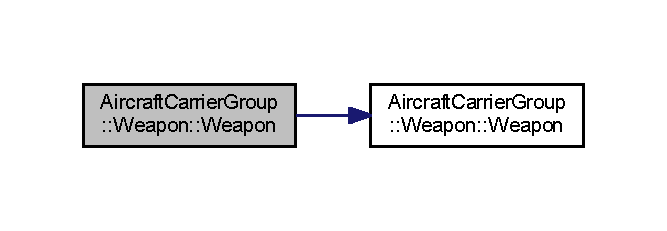
\includegraphics[width=320pt]{class_aircraft_carrier_group_1_1_weapon_a873b32cd3111fc6106d7f13eb4c17e83_cgraph}
\end{center}
\end{figure}
\mbox{\Hypertarget{class_aircraft_carrier_group_1_1_weapon_afd4999fbde839ecc830fc0786ad84b68}\label{class_aircraft_carrier_group_1_1_weapon_afd4999fbde839ecc830fc0786ad84b68}} 
\index{Aircraft\+Carrier\+Group\+::\+Weapon@{Aircraft\+Carrier\+Group\+::\+Weapon}!Weapon@{Weapon}}
\index{Weapon@{Weapon}!Aircraft\+Carrier\+Group\+::\+Weapon@{Aircraft\+Carrier\+Group\+::\+Weapon}}
\subsubsection{\texorpdfstring{Weapon()}{Weapon()}\hspace{0.1cm}{\footnotesize\ttfamily [2/2]}}
{\footnotesize\ttfamily Aircraft\+Carrier\+Group\+::\+Weapon\+::\+Weapon (\begin{DoxyParamCaption}\item[{const \mbox{\hyperlink{class_aircraft_carrier_group_1_1_weapon}{Weapon}} \&}]{Arsenal }\end{DoxyParamCaption})}



Копирующий конструктор 


\begin{DoxyParams}{Parameters}
{\em Arsenal} & Описатель копируемого оружия \\
\hline
\end{DoxyParams}


\subsection{Member Function Documentation}
\mbox{\Hypertarget{class_aircraft_carrier_group_1_1_weapon_a5d8ce784fb56b4f84f028d92dcae7a25}\label{class_aircraft_carrier_group_1_1_weapon_a5d8ce784fb56b4f84f028d92dcae7a25}} 
\index{Aircraft\+Carrier\+Group\+::\+Weapon@{Aircraft\+Carrier\+Group\+::\+Weapon}!Set\+Damage@{Set\+Damage}}
\index{Set\+Damage@{Set\+Damage}!Aircraft\+Carrier\+Group\+::\+Weapon@{Aircraft\+Carrier\+Group\+::\+Weapon}}
\subsubsection{\texorpdfstring{Set\+Damage()}{SetDamage()}}
{\footnotesize\ttfamily \mbox{\hyperlink{class_aircraft_carrier_group_1_1_weapon}{Weapon}}\& Aircraft\+Carrier\+Group\+::\+Weapon\+::\+Set\+Damage (\begin{DoxyParamCaption}\item[{int}]{Damage\+Tmp }\end{DoxyParamCaption})\hspace{0.3cm}{\ttfamily [inline]}}



Устанавливает урон орудия, наносимого по цели за попадание 


\begin{DoxyParams}[1]{Parameters}
\mbox{\tt in}  & {\em Damage\+Tmp} & Обновленный урон \\
\hline
\end{DoxyParams}
\begin{DoxyReturn}{Returns}
Возвращает измененные параметры оружия 
\end{DoxyReturn}
\mbox{\Hypertarget{class_aircraft_carrier_group_1_1_weapon_af026b090b1f5230fdaf68ffcc481eba3}\label{class_aircraft_carrier_group_1_1_weapon_af026b090b1f5230fdaf68ffcc481eba3}} 
\index{Aircraft\+Carrier\+Group\+::\+Weapon@{Aircraft\+Carrier\+Group\+::\+Weapon}!Set\+Munition@{Set\+Munition}}
\index{Set\+Munition@{Set\+Munition}!Aircraft\+Carrier\+Group\+::\+Weapon@{Aircraft\+Carrier\+Group\+::\+Weapon}}
\subsubsection{\texorpdfstring{Set\+Munition()}{SetMunition()}}
{\footnotesize\ttfamily \mbox{\hyperlink{class_aircraft_carrier_group_1_1_weapon}{Weapon}}\& Aircraft\+Carrier\+Group\+::\+Weapon\+::\+Set\+Munition (\begin{DoxyParamCaption}\item[{std\+::string}]{Munition }\end{DoxyParamCaption})\hspace{0.3cm}{\ttfamily [inline]}}



Устанавливает название боеприпаса 


\begin{DoxyParams}[1]{Parameters}
\mbox{\tt in}  & {\em Munition} & Новое название боеприпаса, применимого для этого орудия \\
\hline
\end{DoxyParams}
\begin{DoxyReturn}{Returns}
Возвращает измененные параметры оружия 
\end{DoxyReturn}
\mbox{\Hypertarget{class_aircraft_carrier_group_1_1_weapon_a9fd2fbb263336abbbc9d12c51a9de3c1}\label{class_aircraft_carrier_group_1_1_weapon_a9fd2fbb263336abbbc9d12c51a9de3c1}} 
\index{Aircraft\+Carrier\+Group\+::\+Weapon@{Aircraft\+Carrier\+Group\+::\+Weapon}!Set\+Quantity\+Ammunition@{Set\+Quantity\+Ammunition}}
\index{Set\+Quantity\+Ammunition@{Set\+Quantity\+Ammunition}!Aircraft\+Carrier\+Group\+::\+Weapon@{Aircraft\+Carrier\+Group\+::\+Weapon}}
\subsubsection{\texorpdfstring{Set\+Quantity\+Ammunition()}{SetQuantityAmmunition()}}
{\footnotesize\ttfamily \mbox{\hyperlink{class_aircraft_carrier_group_1_1_weapon}{Weapon}}\& Aircraft\+Carrier\+Group\+::\+Weapon\+::\+Set\+Quantity\+Ammunition (\begin{DoxyParamCaption}\item[{int}]{Quantity\+Ammunition\+Tmp }\end{DoxyParamCaption})\hspace{0.3cm}{\ttfamily [inline]}}



Устанавливает новое количество боеприпасов 


\begin{DoxyParams}[1]{Parameters}
\mbox{\tt in}  & {\em Quantity\+Ammunition\+Tmp} & Новое количество боеприпасов \\
\hline
\end{DoxyParams}
\begin{DoxyReturn}{Returns}
Возвращает измененные параметры оружия 
\end{DoxyReturn}
\mbox{\Hypertarget{class_aircraft_carrier_group_1_1_weapon_a8f83ea62a85411992eb53634fc43b011}\label{class_aircraft_carrier_group_1_1_weapon_a8f83ea62a85411992eb53634fc43b011}} 
\index{Aircraft\+Carrier\+Group\+::\+Weapon@{Aircraft\+Carrier\+Group\+::\+Weapon}!Set\+Rate\+Fire@{Set\+Rate\+Fire}}
\index{Set\+Rate\+Fire@{Set\+Rate\+Fire}!Aircraft\+Carrier\+Group\+::\+Weapon@{Aircraft\+Carrier\+Group\+::\+Weapon}}
\subsubsection{\texorpdfstring{Set\+Rate\+Fire()}{SetRateFire()}}
{\footnotesize\ttfamily \mbox{\hyperlink{class_aircraft_carrier_group_1_1_weapon}{Weapon}}\& Aircraft\+Carrier\+Group\+::\+Weapon\+::\+Set\+Rate\+Fire (\begin{DoxyParamCaption}\item[{int}]{Rate\+Fire\+Tmp }\end{DoxyParamCaption})\hspace{0.3cm}{\ttfamily [inline]}}



Устанавливает скорострельность орудия 


\begin{DoxyParams}[1]{Parameters}
\mbox{\tt in}  & {\em Rate\+Fire\+Tmp} & Новый параметр скорострельности \\
\hline
\end{DoxyParams}
\begin{DoxyReturn}{Returns}
Возвращает измененные параметры оружия 
\end{DoxyReturn}
\mbox{\Hypertarget{class_aircraft_carrier_group_1_1_weapon_a3a73357d6f4f8676192cc10f255e82d2}\label{class_aircraft_carrier_group_1_1_weapon_a3a73357d6f4f8676192cc10f255e82d2}} 
\index{Aircraft\+Carrier\+Group\+::\+Weapon@{Aircraft\+Carrier\+Group\+::\+Weapon}!Set\+Weapon@{Set\+Weapon}}
\index{Set\+Weapon@{Set\+Weapon}!Aircraft\+Carrier\+Group\+::\+Weapon@{Aircraft\+Carrier\+Group\+::\+Weapon}}
\subsubsection{\texorpdfstring{Set\+Weapon()}{SetWeapon()}}
{\footnotesize\ttfamily \mbox{\hyperlink{class_aircraft_carrier_group_1_1_weapon}{Weapon}}\& Aircraft\+Carrier\+Group\+::\+Weapon\+::\+Set\+Weapon (\begin{DoxyParamCaption}\item[{std\+::string}]{Weapon }\end{DoxyParamCaption})\hspace{0.3cm}{\ttfamily [inline]}}



Устанавливает названия оружия 


\begin{DoxyParams}[1]{Parameters}
\mbox{\tt in}  & {\em \mbox{\hyperlink{class_aircraft_carrier_group_1_1_weapon}{Weapon}}} & Новое название оружия \\
\hline
\end{DoxyParams}
\begin{DoxyReturn}{Returns}
Возвращает измененные параметры оружия 
\end{DoxyReturn}
Here is the call graph for this function\+:
\nopagebreak
\begin{figure}[H]
\begin{center}
\leavevmode
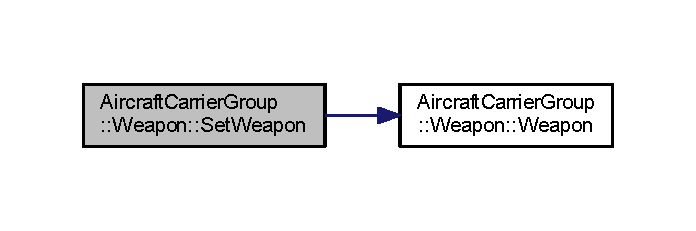
\includegraphics[width=334pt]{class_aircraft_carrier_group_1_1_weapon_a3a73357d6f4f8676192cc10f255e82d2_cgraph}
\end{center}
\end{figure}


The documentation for this class was generated from the following files\+:\begin{DoxyCompactItemize}
\item 
C\+:/\+Users/\+Sema/\+Desktop/\+Code\+Forces/\+Labs/4th\+\_\+\+Lab + library connection/\+Library/\mbox{\hyperlink{_weapon_8h}{Weapon.\+h}}\item 
C\+:/\+Users/\+Sema/\+Desktop/\+Code\+Forces/\+Labs/4th\+\_\+\+Lab + library connection/\+Library/Weapon.\+cpp\end{DoxyCompactItemize}

\chapter{File Documentation}
\hypertarget{_aircraft_8h}{}\section{C\+:/\+Users/\+Sema/\+Desktop/\+Code\+Forces/\+Labs/4th\+\_\+\+Lab + library connection/\+Library/\+Aircraft.h File Reference}
\label{_aircraft_8h}\index{C\+:/\+Users/\+Sema/\+Desktop/\+Code\+Forces/\+Labs/4th\+\_\+\+Lab + library connection/\+Library/\+Aircraft.\+h@{C\+:/\+Users/\+Sema/\+Desktop/\+Code\+Forces/\+Labs/4th\+\_\+\+Lab + library connection/\+Library/\+Aircraft.\+h}}


Заголовочный файл с описанием класса  Данный файл содержит в себе определение класса Aircraft.  


{\ttfamily \#include $<$iostream$>$}\newline
{\ttfamily \#include $<$fstream$>$}\newline
{\ttfamily \#include \char`\"{}Weapon.\+h\char`\"{}}\newline
{\ttfamily \#include \char`\"{}Military\+Characteristics.\+h\char`\"{}}\newline
Include dependency graph for Aircraft.\+h\+:
\nopagebreak
\begin{figure}[H]
\begin{center}
\leavevmode
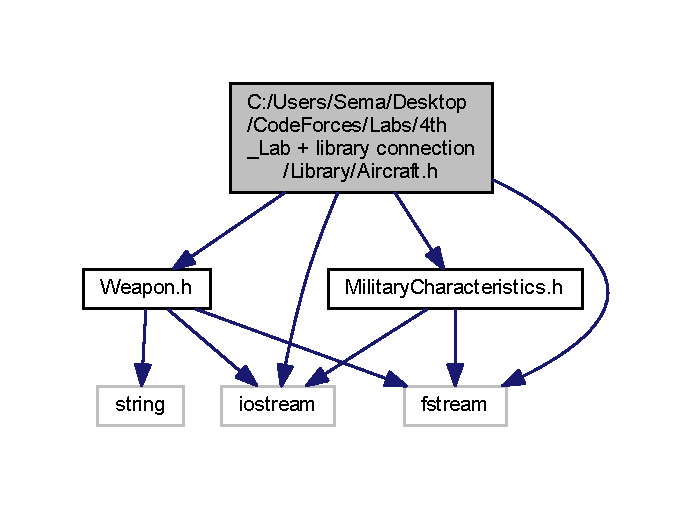
\includegraphics[width=332pt]{_aircraft_8h__incl}
\end{center}
\end{figure}
This graph shows which files directly or indirectly include this file\+:
\nopagebreak
\begin{figure}[H]
\begin{center}
\leavevmode
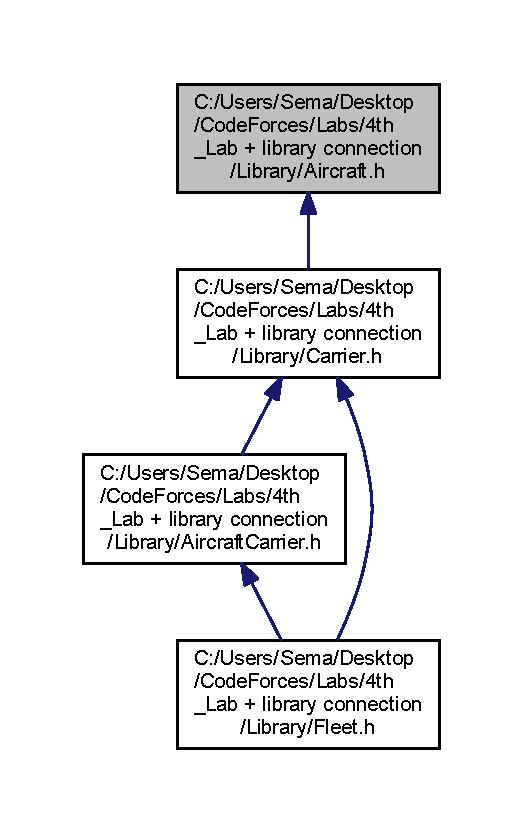
\includegraphics[width=251pt]{_aircraft_8h__dep__incl}
\end{center}
\end{figure}
\subsection*{Classes}
\begin{DoxyCompactItemize}
\item 
class \mbox{\hyperlink{class_aircraft_carrier_group_1_1_aircraft}{Aircraft\+Carrier\+Group\+::\+Aircraft}}
\begin{DoxyCompactList}\small\item\em Класс для описания самолета  Осуществляет хранение всех параметров самолета и содержит функции, обрабатывающие эти параметры \end{DoxyCompactList}\end{DoxyCompactItemize}
\subsection*{Namespaces}
\begin{DoxyCompactItemize}
\item 
 \mbox{\hyperlink{namespace_aircraft_carrier_group}{Aircraft\+Carrier\+Group}}
\begin{DoxyCompactList}\small\item\em Пространство имен \mbox{\hyperlink{namespace_aircraft_carrier_group}{Aircraft\+Carrier\+Group}}. \end{DoxyCompactList}\end{DoxyCompactItemize}


\subsection{Detailed Description}
Заголовочный файл с описанием класса  Данный файл содержит в себе определение класса Aircraft. 


\hypertarget{_aircraft_carrier_8h}{}\section{C\+:/\+Users/\+Sema/\+Desktop/\+Code\+Forces/\+Labs/4th\+\_\+\+Lab + library connection/\+Library/\+Aircraft\+Carrier.h File Reference}
\label{_aircraft_carrier_8h}\index{C\+:/\+Users/\+Sema/\+Desktop/\+Code\+Forces/\+Labs/4th\+\_\+\+Lab + library connection/\+Library/\+Aircraft\+Carrier.\+h@{C\+:/\+Users/\+Sema/\+Desktop/\+Code\+Forces/\+Labs/4th\+\_\+\+Lab + library connection/\+Library/\+Aircraft\+Carrier.\+h}}


Заголовочный файл с описанием класса  Данный файл содержит в себе определение класса Aircraft\+Carrier.  


{\ttfamily \#include $<$iostream$>$}\newline
{\ttfamily \#include \char`\"{}Carrier.\+h\char`\"{}}\newline
Include dependency graph for Aircraft\+Carrier.\+h\+:
\nopagebreak
\begin{figure}[H]
\begin{center}
\leavevmode
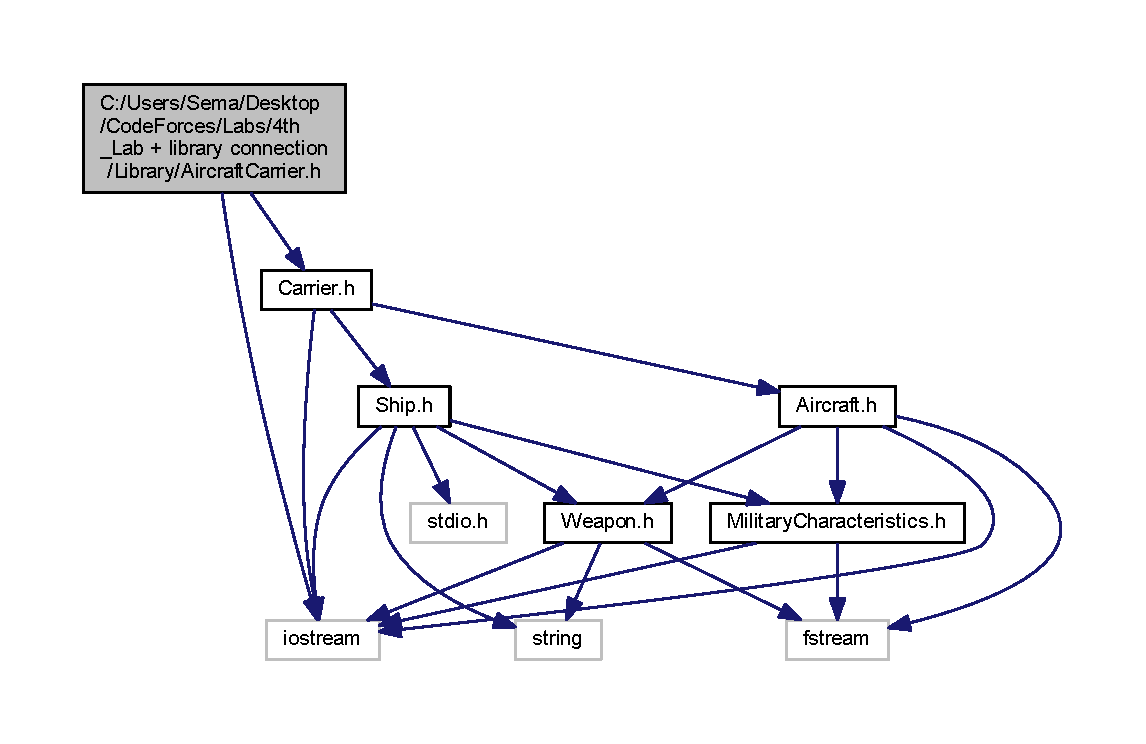
\includegraphics[width=350pt]{_aircraft_carrier_8h__incl}
\end{center}
\end{figure}
This graph shows which files directly or indirectly include this file\+:
\nopagebreak
\begin{figure}[H]
\begin{center}
\leavevmode
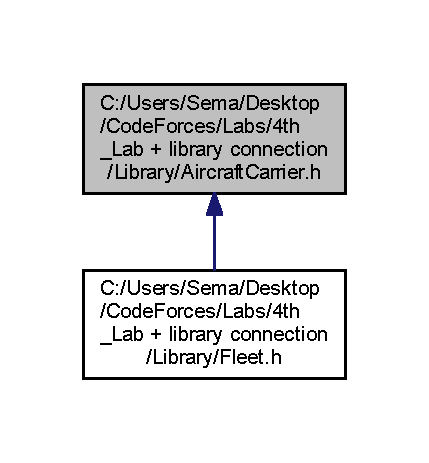
\includegraphics[width=206pt]{_aircraft_carrier_8h__dep__incl}
\end{center}
\end{figure}
\subsection*{Classes}
\begin{DoxyCompactItemize}
\item 
class \mbox{\hyperlink{class_aircraft_carrier_group_1_1_aircraft_carrier}{Aircraft\+Carrier\+Group\+::\+Aircraft\+Carrier}}
\begin{DoxyCompactList}\small\item\em Класс для описания авианесущего крейсера  Осуществляет хранение всех параметров авианесущего крейсера и содержит функции, обрабатывающие эти параметры \end{DoxyCompactList}\end{DoxyCompactItemize}
\subsection*{Namespaces}
\begin{DoxyCompactItemize}
\item 
 \mbox{\hyperlink{namespace_aircraft_carrier_group}{Aircraft\+Carrier\+Group}}
\begin{DoxyCompactList}\small\item\em Пространство имен \mbox{\hyperlink{namespace_aircraft_carrier_group}{Aircraft\+Carrier\+Group}}. \end{DoxyCompactList}\end{DoxyCompactItemize}


\subsection{Detailed Description}
Заголовочный файл с описанием класса  Данный файл содержит в себе определение класса Aircraft\+Carrier. 


\hypertarget{_carrier_8h}{}\section{C\+:/\+Users/\+Sema/\+Desktop/\+Code\+Forces/\+Labs/4th\+\_\+\+Lab + library connection/\+Library/\+Carrier.h File Reference}
\label{_carrier_8h}\index{C\+:/\+Users/\+Sema/\+Desktop/\+Code\+Forces/\+Labs/4th\+\_\+\+Lab + library connection/\+Library/\+Carrier.\+h@{C\+:/\+Users/\+Sema/\+Desktop/\+Code\+Forces/\+Labs/4th\+\_\+\+Lab + library connection/\+Library/\+Carrier.\+h}}


Заголовочный файл с описанием класса  Данный файл содержит в себе определение класса Carrier.  


{\ttfamily \#include $<$iostream$>$}\newline
{\ttfamily \#include \char`\"{}Ship.\+h\char`\"{}}\newline
{\ttfamily \#include \char`\"{}Aircraft.\+h\char`\"{}}\newline
Include dependency graph for Carrier.\+h\+:
\nopagebreak
\begin{figure}[H]
\begin{center}
\leavevmode
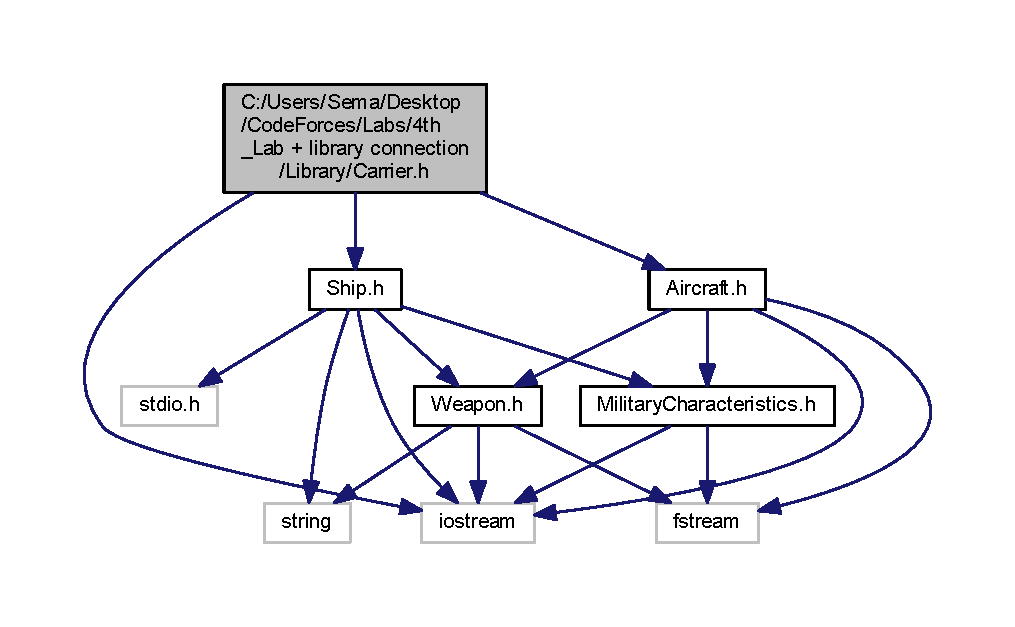
\includegraphics[width=350pt]{_carrier_8h__incl}
\end{center}
\end{figure}
This graph shows which files directly or indirectly include this file\+:
\nopagebreak
\begin{figure}[H]
\begin{center}
\leavevmode
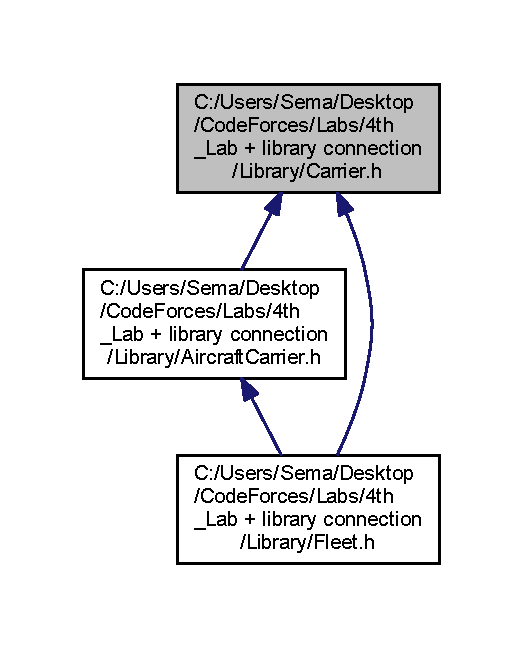
\includegraphics[width=251pt]{_carrier_8h__dep__incl}
\end{center}
\end{figure}
\subsection*{Classes}
\begin{DoxyCompactItemize}
\item 
class \mbox{\hyperlink{class_aircraft_carrier_group_1_1_carrier}{Aircraft\+Carrier\+Group\+::\+Carrier}}
\begin{DoxyCompactList}\small\item\em Класс для описания авианосца  Осуществляет хранение всех параметров авиносца и содержит функции, обрабатывающие эти параметры \end{DoxyCompactList}\end{DoxyCompactItemize}
\subsection*{Namespaces}
\begin{DoxyCompactItemize}
\item 
 \mbox{\hyperlink{namespace_aircraft_carrier_group}{Aircraft\+Carrier\+Group}}
\begin{DoxyCompactList}\small\item\em Пространство имен \mbox{\hyperlink{namespace_aircraft_carrier_group}{Aircraft\+Carrier\+Group}}. \end{DoxyCompactList}\end{DoxyCompactItemize}


\subsection{Detailed Description}
Заголовочный файл с описанием класса  Данный файл содержит в себе определение класса Carrier. 


\hypertarget{_cover_ship_8h}{}\section{C\+:/\+Users/\+Sema/\+Desktop/\+Code\+Forces/\+Labs/4th\+\_\+\+Lab + library connection/\+Library/\+Cover\+Ship.h File Reference}
\label{_cover_ship_8h}\index{C\+:/\+Users/\+Sema/\+Desktop/\+Code\+Forces/\+Labs/4th\+\_\+\+Lab + library connection/\+Library/\+Cover\+Ship.\+h@{C\+:/\+Users/\+Sema/\+Desktop/\+Code\+Forces/\+Labs/4th\+\_\+\+Lab + library connection/\+Library/\+Cover\+Ship.\+h}}


Заголовочный файл с описанием класса  Данный файл содержит в себе определение класса Cover\+Ship.  


{\ttfamily \#include $<$iostream$>$}\newline
{\ttfamily \#include $<$fstream$>$}\newline
{\ttfamily \#include \char`\"{}Ship.\+h\char`\"{}}\newline
Include dependency graph for Cover\+Ship.\+h\+:
\nopagebreak
\begin{figure}[H]
\begin{center}
\leavevmode
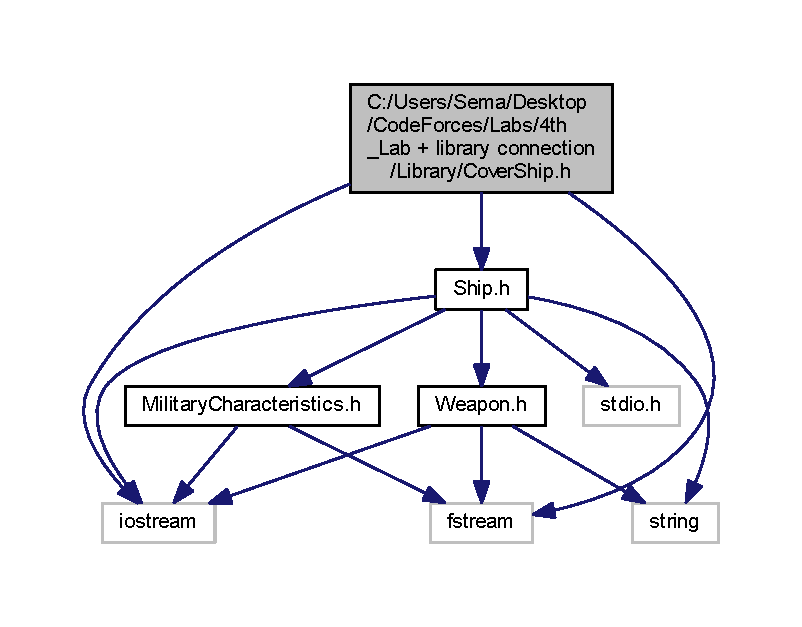
\includegraphics[width=350pt]{_cover_ship_8h__incl}
\end{center}
\end{figure}
This graph shows which files directly or indirectly include this file\+:
\nopagebreak
\begin{figure}[H]
\begin{center}
\leavevmode
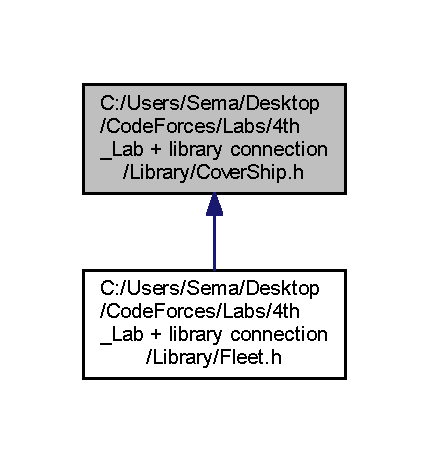
\includegraphics[width=206pt]{_cover_ship_8h__dep__incl}
\end{center}
\end{figure}
\subsection*{Classes}
\begin{DoxyCompactItemize}
\item 
class \mbox{\hyperlink{class_aircraft_carrier_group_1_1_cover_ship}{Aircraft\+Carrier\+Group\+::\+Cover\+Ship}}
\begin{DoxyCompactList}\small\item\em Класс для описания судна прикрытия  Осуществляет хранение всех параметров судна прикрытия и содержит функции, обрабатывающие эти параметры \end{DoxyCompactList}\end{DoxyCompactItemize}
\subsection*{Namespaces}
\begin{DoxyCompactItemize}
\item 
 \mbox{\hyperlink{namespace_aircraft_carrier_group}{Aircraft\+Carrier\+Group}}
\begin{DoxyCompactList}\small\item\em Пространство имен \mbox{\hyperlink{namespace_aircraft_carrier_group}{Aircraft\+Carrier\+Group}}. \end{DoxyCompactList}\end{DoxyCompactItemize}


\subsection{Detailed Description}
Заголовочный файл с описанием класса  Данный файл содержит в себе определение класса Cover\+Ship. 


\hypertarget{_fleet_8h}{}\section{C\+:/\+Users/\+Sema/\+Desktop/\+Code\+Forces/\+Labs/4th\+\_\+\+Lab + library connection/\+Library/\+Fleet.h File Reference}
\label{_fleet_8h}\index{C\+:/\+Users/\+Sema/\+Desktop/\+Code\+Forces/\+Labs/4th\+\_\+\+Lab + library connection/\+Library/\+Fleet.\+h@{C\+:/\+Users/\+Sema/\+Desktop/\+Code\+Forces/\+Labs/4th\+\_\+\+Lab + library connection/\+Library/\+Fleet.\+h}}


Заголовочный файл с описанием класса и его итератора  Данный файл содержит в себе определение класса Fleet.  


{\ttfamily \#include \char`\"{}\+\_\+map.\+h\char`\"{}}\newline
{\ttfamily \#include $<$iostream$>$}\newline
{\ttfamily \#include $<$fstream$>$}\newline
{\ttfamily \#include \char`\"{}Ship.\+h\char`\"{}}\newline
{\ttfamily \#include \char`\"{}Cover\+Ship.\+h\char`\"{}}\newline
{\ttfamily \#include \char`\"{}Carrier.\+h\char`\"{}}\newline
{\ttfamily \#include \char`\"{}Aircraft\+Carrier.\+h\char`\"{}}\newline
Include dependency graph for Fleet.\+h\+:
\nopagebreak
\begin{figure}[H]
\begin{center}
\leavevmode
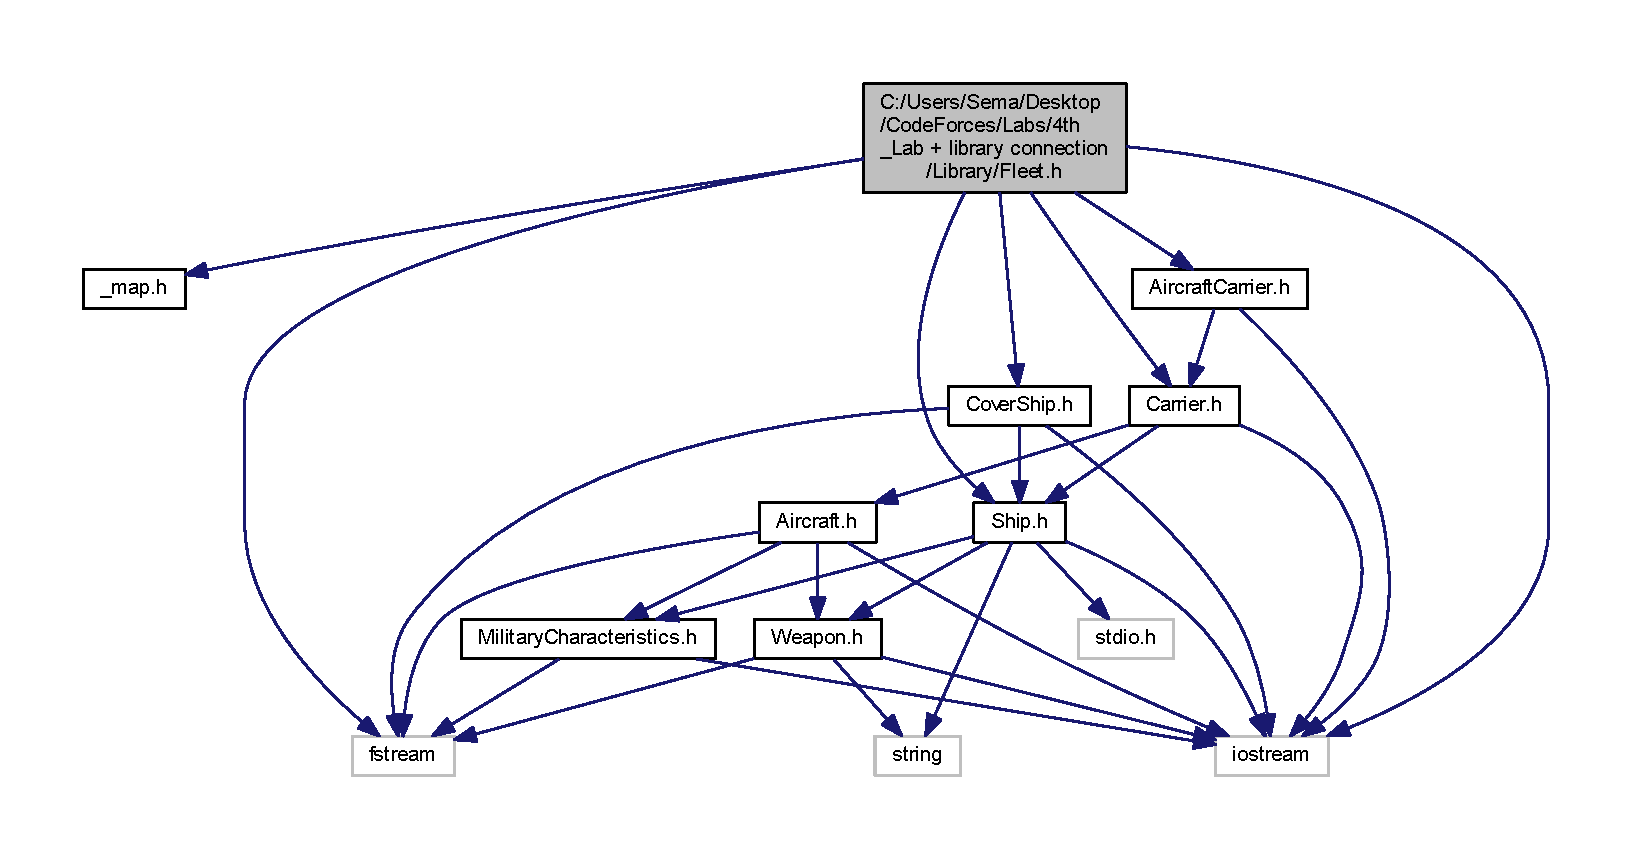
\includegraphics[width=350pt]{_fleet_8h__incl}
\end{center}
\end{figure}
\subsection*{Classes}
\begin{DoxyCompactItemize}
\item 
class \mbox{\hyperlink{class_aircraft_carrier_group_1_1_const_fleet_it}{Aircraft\+Carrier\+Group\+::\+Const\+Fleet\+It}}
\begin{DoxyCompactList}\small\item\em Класс-\/итератор для класса \mbox{\hyperlink{class_aircraft_carrier_group_1_1_fleet}{Fleet}}  При его помощи осуществляется доступ к элементам контейнера класса \mbox{\hyperlink{class_aircraft_carrier_group_1_1_fleet}{Fleet}}. \end{DoxyCompactList}\item 
class \mbox{\hyperlink{class_aircraft_carrier_group_1_1_fleet}{Aircraft\+Carrier\+Group\+::\+Fleet}}
\begin{DoxyCompactList}\small\item\em Класс для описания флота  Осуществляет хранение описателей всех кораблей флота и содержит функции, позволяющие взаимодействовать с кораблями флота \end{DoxyCompactList}\end{DoxyCompactItemize}
\subsection*{Namespaces}
\begin{DoxyCompactItemize}
\item 
 \mbox{\hyperlink{namespace_aircraft_carrier_group}{Aircraft\+Carrier\+Group}}
\begin{DoxyCompactList}\small\item\em Пространство имен \mbox{\hyperlink{namespace_aircraft_carrier_group}{Aircraft\+Carrier\+Group}}. \end{DoxyCompactList}\end{DoxyCompactItemize}


\subsection{Detailed Description}
Заголовочный файл с описанием класса и его итератора  Данный файл содержит в себе определение класса Fleet. 


\hypertarget{_military_characteristics_8h}{}\section{C\+:/\+Users/\+Sema/\+Desktop/\+Code\+Forces/\+Labs/4th\+\_\+\+Lab + library connection/\+Library/\+Military\+Characteristics.h File Reference}
\label{_military_characteristics_8h}\index{C\+:/\+Users/\+Sema/\+Desktop/\+Code\+Forces/\+Labs/4th\+\_\+\+Lab + library connection/\+Library/\+Military\+Characteristics.\+h@{C\+:/\+Users/\+Sema/\+Desktop/\+Code\+Forces/\+Labs/4th\+\_\+\+Lab + library connection/\+Library/\+Military\+Characteristics.\+h}}


Заголовочный файл с описанием класса  Данный файл содержит в себе определение класса Military\+Characteristics.  


{\ttfamily \#include $<$iostream$>$}\newline
{\ttfamily \#include $<$fstream$>$}\newline
Include dependency graph for Military\+Characteristics.\+h\+:
\nopagebreak
\begin{figure}[H]
\begin{center}
\leavevmode
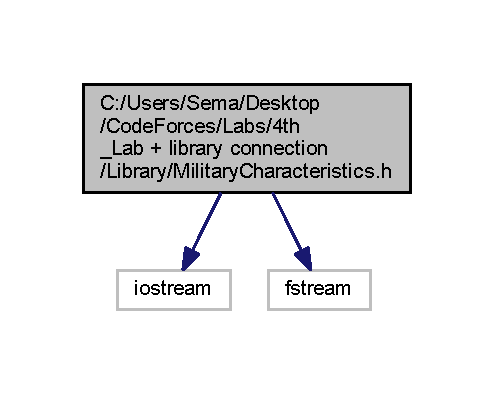
\includegraphics[width=237pt]{_military_characteristics_8h__incl}
\end{center}
\end{figure}
This graph shows which files directly or indirectly include this file\+:
\nopagebreak
\begin{figure}[H]
\begin{center}
\leavevmode
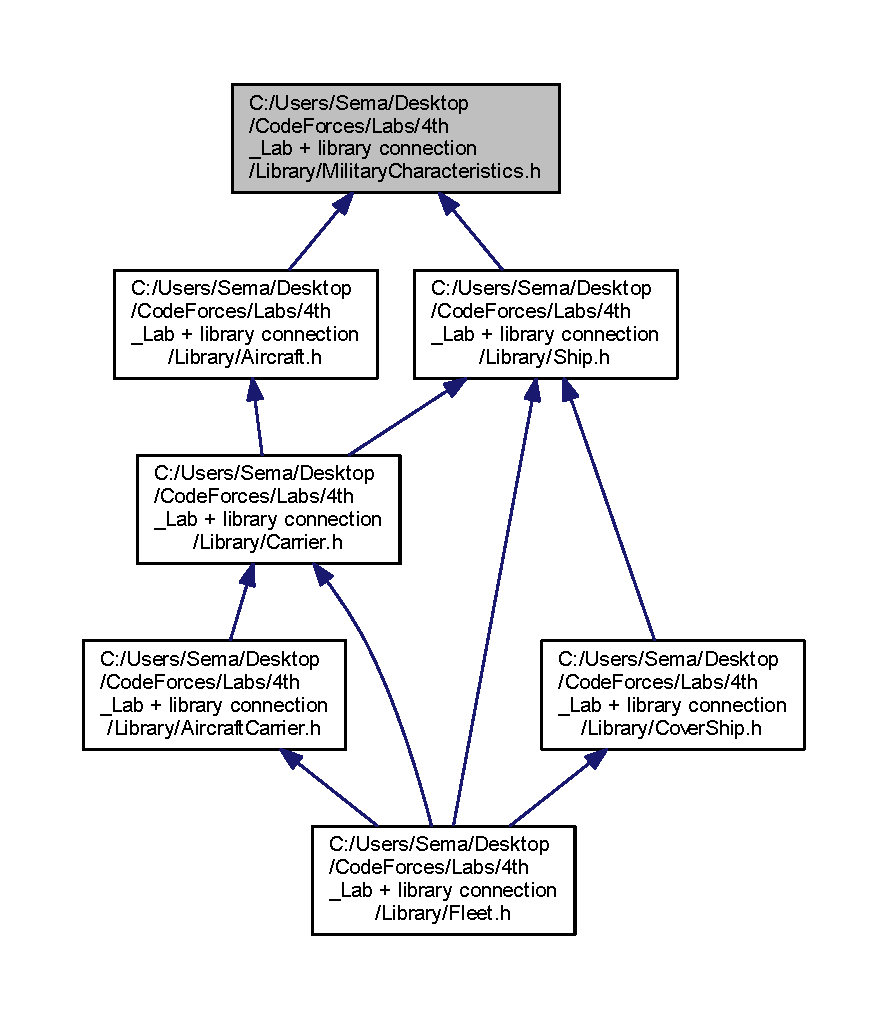
\includegraphics[width=350pt]{_military_characteristics_8h__dep__incl}
\end{center}
\end{figure}
\subsection*{Classes}
\begin{DoxyCompactItemize}
\item 
class \mbox{\hyperlink{class_aircraft_carrier_group_1_1_military_characteristics}{Aircraft\+Carrier\+Group\+::\+Military\+Characteristics}}
\begin{DoxyCompactList}\small\item\em Класс для описания некоторых парметров техники  Осуществляет хранение и обработку некоторых характеристик техники \end{DoxyCompactList}\end{DoxyCompactItemize}
\subsection*{Namespaces}
\begin{DoxyCompactItemize}
\item 
 \mbox{\hyperlink{namespace_aircraft_carrier_group}{Aircraft\+Carrier\+Group}}
\begin{DoxyCompactList}\small\item\em Пространство имен \mbox{\hyperlink{namespace_aircraft_carrier_group}{Aircraft\+Carrier\+Group}}. \end{DoxyCompactList}\end{DoxyCompactItemize}


\subsection{Detailed Description}
Заголовочный файл с описанием класса  Данный файл содержит в себе определение класса Military\+Characteristics. 


\hypertarget{_ship_8h}{}\section{C\+:/\+Users/\+Sema/\+Desktop/\+Code\+Forces/\+Labs/4th\+\_\+\+Lab + library connection/\+Library/\+Ship.h File Reference}
\label{_ship_8h}\index{C\+:/\+Users/\+Sema/\+Desktop/\+Code\+Forces/\+Labs/4th\+\_\+\+Lab + library connection/\+Library/\+Ship.\+h@{C\+:/\+Users/\+Sema/\+Desktop/\+Code\+Forces/\+Labs/4th\+\_\+\+Lab + library connection/\+Library/\+Ship.\+h}}


Заголовочный файл с описанием класса  Данный файл содержит в себе определение класса Cover\+Ship.  


{\ttfamily \#include $<$string$>$}\newline
{\ttfamily \#include $<$iostream$>$}\newline
{\ttfamily \#include \char`\"{}stdio.\+h\char`\"{}}\newline
{\ttfamily \#include \char`\"{}Weapon.\+h\char`\"{}}\newline
{\ttfamily \#include \char`\"{}Military\+Characteristics.\+h\char`\"{}}\newline
Include dependency graph for Ship.\+h\+:
\nopagebreak
\begin{figure}[H]
\begin{center}
\leavevmode
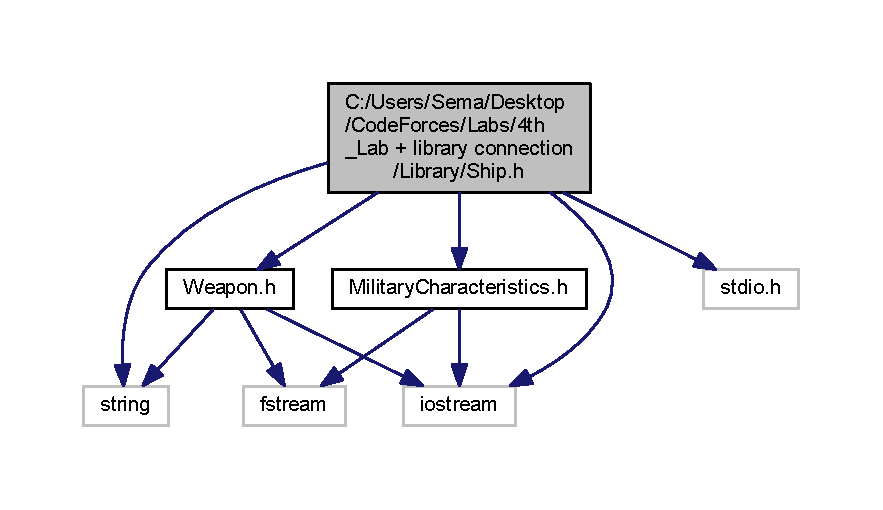
\includegraphics[width=350pt]{_ship_8h__incl}
\end{center}
\end{figure}
This graph shows which files directly or indirectly include this file\+:
\nopagebreak
\begin{figure}[H]
\begin{center}
\leavevmode
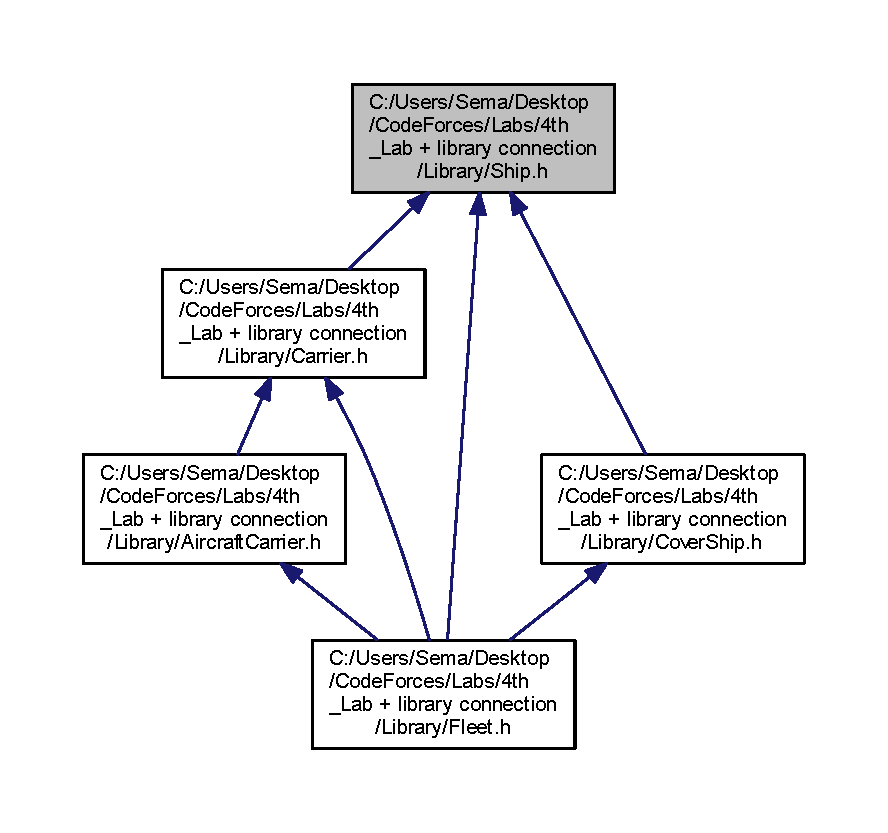
\includegraphics[width=350pt]{_ship_8h__dep__incl}
\end{center}
\end{figure}
\subsection*{Classes}
\begin{DoxyCompactItemize}
\item 
struct \mbox{\hyperlink{struct_aircraft_carrier_group_1_1_captain}{Aircraft\+Carrier\+Group\+::\+Captain}}
\begin{DoxyCompactList}\small\item\em Структура для описания капитана  Осуществляет хранение всех параметров командира судна или флота \end{DoxyCompactList}\item 
class \mbox{\hyperlink{class_aircraft_carrier_group_1_1_ship}{Aircraft\+Carrier\+Group\+::\+Ship}}
\begin{DoxyCompactList}\small\item\em Абстрактный класс для описания кораблей  Осуществляет хранение общих параметров кораблей и содержит функции, обрабатывающие эти параметры \end{DoxyCompactList}\end{DoxyCompactItemize}
\subsection*{Namespaces}
\begin{DoxyCompactItemize}
\item 
 \mbox{\hyperlink{namespace_aircraft_carrier_group}{Aircraft\+Carrier\+Group}}
\begin{DoxyCompactList}\small\item\em Пространство имен \mbox{\hyperlink{namespace_aircraft_carrier_group}{Aircraft\+Carrier\+Group}}. \end{DoxyCompactList}\end{DoxyCompactItemize}
\subsection*{Variables}
\begin{DoxyCompactItemize}
\item 
\mbox{\Hypertarget{namespace_aircraft_carrier_group_a450635cd66c0fbcc37535160a56142b8}\label{namespace_aircraft_carrier_group_a450635cd66c0fbcc37535160a56142b8}} 
const double {\bfseries Aircraft\+Carrier\+Group\+::eps} = 1e-\/9
\end{DoxyCompactItemize}


\subsection{Detailed Description}
Заголовочный файл с описанием класса  Данный файл содержит в себе определение класса Cover\+Ship. 


\hypertarget{_weapon_8h}{}\section{C\+:/\+Users/\+Sema/\+Desktop/\+Code\+Forces/\+Labs/4th\+\_\+\+Lab + library connection/\+Library/\+Weapon.h File Reference}
\label{_weapon_8h}\index{C\+:/\+Users/\+Sema/\+Desktop/\+Code\+Forces/\+Labs/4th\+\_\+\+Lab + library connection/\+Library/\+Weapon.\+h@{C\+:/\+Users/\+Sema/\+Desktop/\+Code\+Forces/\+Labs/4th\+\_\+\+Lab + library connection/\+Library/\+Weapon.\+h}}


Заголовочный файл с описанием класса  Данный файл содержит в себе определение класса Weapon.  


{\ttfamily \#include $<$iostream$>$}\newline
{\ttfamily \#include $<$fstream$>$}\newline
{\ttfamily \#include $<$string$>$}\newline
Include dependency graph for Weapon.\+h\+:
\nopagebreak
\begin{figure}[H]
\begin{center}
\leavevmode
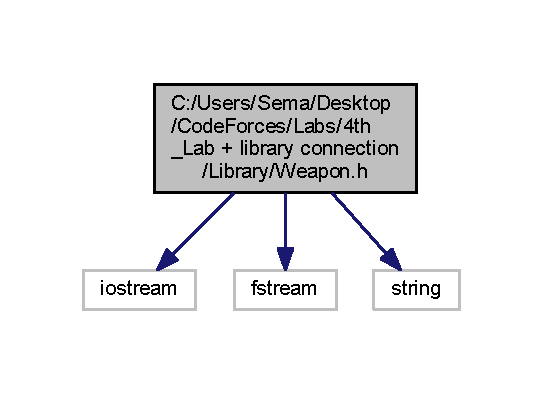
\includegraphics[width=261pt]{_weapon_8h__incl}
\end{center}
\end{figure}
This graph shows which files directly or indirectly include this file\+:
\nopagebreak
\begin{figure}[H]
\begin{center}
\leavevmode
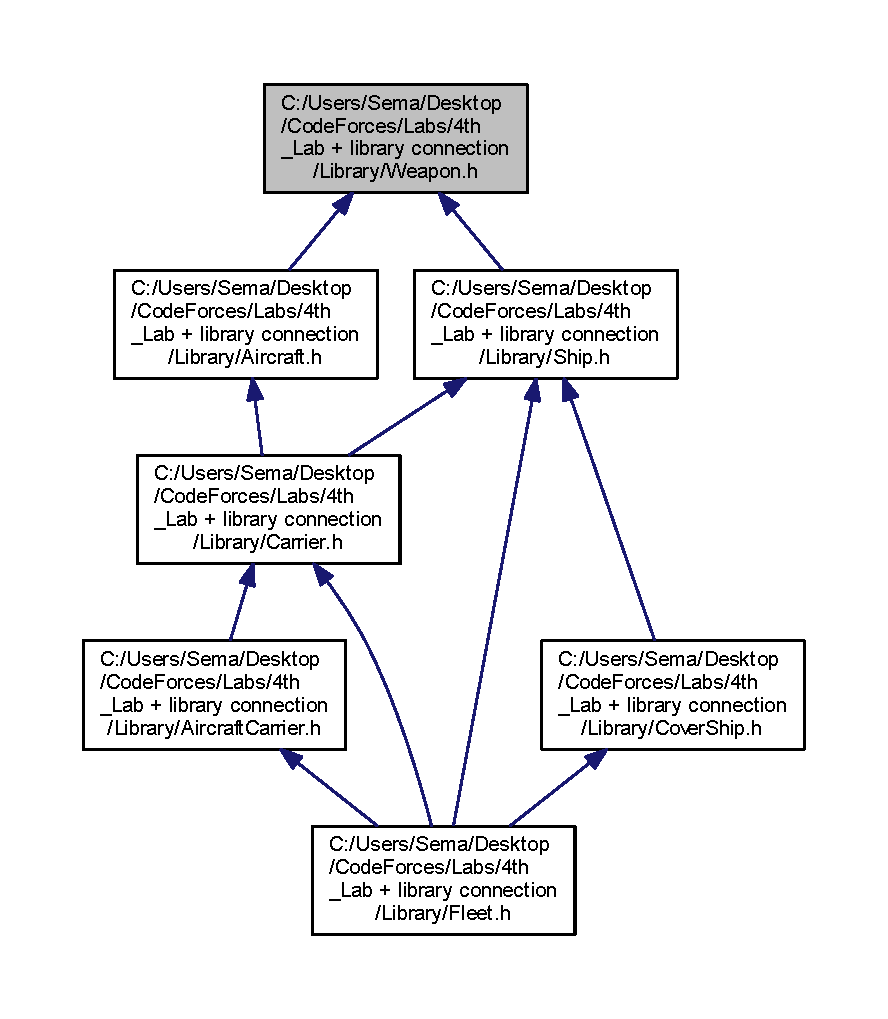
\includegraphics[width=350pt]{_weapon_8h__dep__incl}
\end{center}
\end{figure}
\subsection*{Classes}
\begin{DoxyCompactItemize}
\item 
class \mbox{\hyperlink{class_aircraft_carrier_group_1_1_weapon}{Aircraft\+Carrier\+Group\+::\+Weapon}}
\begin{DoxyCompactList}\small\item\em Класс для описания вооружения  Осуществляет хранение всех параметров авианесущего крейсера и содержит функции, обрабатывающие эти параметры \end{DoxyCompactList}\end{DoxyCompactItemize}
\subsection*{Namespaces}
\begin{DoxyCompactItemize}
\item 
 \mbox{\hyperlink{namespace_aircraft_carrier_group}{Aircraft\+Carrier\+Group}}
\begin{DoxyCompactList}\small\item\em Пространство имен \mbox{\hyperlink{namespace_aircraft_carrier_group}{Aircraft\+Carrier\+Group}}. \end{DoxyCompactList}\end{DoxyCompactItemize}


\subsection{Detailed Description}
Заголовочный файл с описанием класса  Данный файл содержит в себе определение класса Weapon. 


%--- End generated contents ---

% Index
\backmatter
\newpage
\phantomsection
\clearemptydoublepage
\addcontentsline{toc}{chapter}{Index}
\printindex

\end{document}
